\documentclass[12pt]{article}  

%%%%%%%% PREÁMBULO %%%%%%%%%%%%
\title{Plantilla para prácticas de UPIITA}
\usepackage[spanish, es-tabla]{babel} %Indica que escribiermos en español
\usepackage[utf8]{inputenc} %Indica qué codificación se está usando ISO-8859-1(latin1)  o utf8  
\usepackage{amsmath} % Comandos extras para matemáticas (cajas para ecuaciones,
% etc)
\usepackage{amssymb} % Simbolos matematicos (por lo tanto)
\usepackage{graphicx} % Incluir imágenes en LaTeX
\usepackage{color} % Para colorear texto
\usepackage{subfigure} % subfiguras
\usepackage{float} %Podemos usar el especificador [H] en las figuras para que se
% queden donde queramos
\usepackage{capt-of} % Permite usar etiquetas fuera de elementos flotantes
% (etiquetas de figuras)
\usepackage{sidecap} % Para poner el texto de las imágenes al lado
	\sidecaptionvpos{figure}{c} % Para que el texto se alinie al centro vertical
\usepackage{caption} % Para poder quitar numeracion de figuras
\usepackage{listofitems}

\usepackage{commath} % funcionalidades extras para diferenciales, integrales,
% etc (\od, \dif, etc)
\usepackage{cancel} % para cancelar expresiones (\cancelto{0}{x})
 
\usepackage{anysize} 					% Para personalizar el ancho de  los márgenes
\marginsize{3cm}{2.5cm}{2.5cm}{2.5cm} % Izquierda, derecha, arriba, abajo

\usepackage{appendix}
\renewcommand{\appendixname}{Apéndices}
\renewcommand{\appendixtocname}{Apéndices}
\renewcommand{\appendixpagename}{Apéndices} 

% Para que las referencias sean hipervínculos a las figuras o ecuaciones y
% aparezcan en color
\usepackage[colorlinks=true,plainpages=true,citecolor=blue,linkcolor=blue]{hyperref}
%\usepackage{hyperref} 
% Para agregar encabezado y pie de página
\usepackage{fancyhdr} 
\pagestyle{fancy}
\fancyhf{}
\fancyhead[L]{\footnotesize UPIITA} %encabezado izquierda
\fancyhead[R]{\footnotesize IPN}   % dereecha
\fancyfoot[R]{\footnotesize Trabajo Terminal}  % Pie derecha
\fancyfoot[C]{\thepage}  % centro
\fancyfoot[L]{\footnotesize Ing. Energía}  %izquierda
\renewcommand{\footrulewidth}{0.4pt}


\usepackage{listings} % Para usar código fuente
\definecolor{dkgreen}{rgb}{0,0.6,0} % Definimos colores para usar en el código
\definecolor{gray}{rgb}{0.5,0.5,0.5} 
% configuración para el lenguaje que queramos utilizar
\lstset{language=Matlab,
   keywords={break,case,catch,continue,else,elseif,end,for,function,
      global,if,otherwise,persistent,return,switch,try,while},
   basicstyle=\ttfamily,
   keywordstyle=\color{blue},
   commentstyle=\color{red},
   stringstyle=\color{dkgreen},
   numbers=left,
   numberstyle=\tiny\color{gray},
   stepnumber=1,
   numbersep=10pt,
   backgroundcolor=\color{white},
   tabsize=4,
   showspaces=false,
   showstringspaces=false}

\newcommand{\sen}{\operatorname{\sen}}	% Definimos el comando \sen para el seno
%en español

\makeatletter
\newcommand{\listofillustrations}{%
    \section*{\listfigurename}
    \begin{itemize}
    \@starttoc{lof}
    \end{itemize}
}
\makeatother


\makeatletter
\newcommand{\listoftablesandmatrices}{%
    \section*{\listtablename}
    \begingroup
    \setsepchar{,}
    \readlist*\tablelist{\@lot}
    \renewcommand*{\do}[1]{\item \tablename~##1: \captionof{table}{\tablelist[##1]}}%
    \begin{itemize}\tablelist\end{itemize}
    \endgroup
}
\makeatother

\title{Plantilla para trabajo terminal I de UPIITA}

%%%%%%%% TERMINA PREÁMBULO %%%%%%%%%%%%
\usepackage{setspace}
\onehalfspacing % Establece el interlineado en 1.5
\renewcommand*\familydefault{\sfdefault} % Cambia la familia de fuente predeterminada a sans-serif (Arial)

\begin{document} 
\pagenumbering{gobble}
%%%%%%%%%%%%%%%%%%%%%%%%%%%%%%%%%% PORTADA %%%%%%%%%%%%%%%%%%%%%%%%%%%%%%%%%%%%%%%%%%%%
																					%%%
\begin{center}																		%%%
\newcommand{\HRule}{\rule{\linewidth}{0.5mm}}									%%%\left
 																					%%%
\begin{minipage}{0.48\textwidth} \begin{flushleft}

\includegraphics[scale = 0.4]{Imagenes/logo_upiita}
\end{flushleft}\end{minipage}
\begin{minipage}{0.48\textwidth} \begin{flushright}

\includegraphics[scale = 0.25]{Imagenes/IPN}
\end{flushright}\end{minipage}

													 								%%%
\vspace*{-1.5cm}								%%%
																					%%%	
\textsc{\huge Instituto Polit\'ecnico\\ \vspace{5px} Nacional}\\[1.5cm]	

\textsc{\LARGE Unidad Profesional Interdisciplinaria en Ingenier\'ia y				%%%
Tecnolog\'ias Avanzadas}\\[1.5cm]													%%%

\begin{minipage}{0.9\textwidth} 
\begin{center}																					%%%
\textsc{\LARGE Trabajo Terminal}
\end{center}
\end{minipage}\\[0.5cm]
%%%
    																				%%%
 			\vspace*{1cm}																		%%%
																					%%%
\HRule \\[0.4cm]																	%%%
{ \huge \bfseries Síntesis de nanocompuestos basados en nano hojas de óxido de grafeno (GO) y semiconductores inorgánicos para aplicaciones en fotocatálisis}\\[0.4cm]	%%%
 																					%%%
\HRule \\[1.5cm]																	%%%
 																				%%%
																					%%%
\begin{minipage}{0.46\textwidth}													%%%
\begin{flushleft} \large															%%%
\emph{Presenta la alumna:}\\	
Becerril Tapia Liliana
%%%
			%\vspace*{2cm}	
            													%%%
										 						%%%
\end{flushleft}																		%%%
\end{minipage}		
																%%%
\begin{minipage}{0.52\textwidth}		
\vspace{-0.7cm}											%%%
\begin{flushright} \large															%%%
\emph{Asesores:} \\																	%%%
Dra. Yazmín Mariela Hernández Rodríguez\\
Dr. Oscar Eduardo Cigarroa Mayorga\\
Dr. Manuel Alejandro Pérez Guzmán													%%%
\end{flushright}																	%%%
\end{minipage}	
\vspace*{0.5cm}
%\begin{flushleft}
 	
%\end{flushleft}
%%%
 		\flushleft{\textbf{\Large Ing. Energía}	}\\																		%%%
\vspace{0.5cm} 																				
\begin{center}																					
{\large \today}																	%%%
 			\end{center}												  						
\end{center}							 											
																					
\newpage	
\pagenumbering{gobble}
%%%%%%%%%%%%%%%%%%%%%%%%%%%%%%%%%% PORTADA %%%%%%%%%%%%%%%%%%%%%%%%%%%%%%%%%%%%%%%%%%%%
																					%%%
\begin{center}																		%%%
\newcommand{\HRule}{\rule{\linewidth}{0.1mm}}									%%%\left
 																					%%%
\begin{minipage}{0.48\textwidth} \begin{flushleft}

\includegraphics[scale = 0.4]{Imagenes/logo_upiita}
\end{flushleft}\end{minipage}
\begin{minipage}{0.48\textwidth} \begin{flushright}

\includegraphics[scale = 0.25]{Imagenes/IPN}
\end{flushright}\end{minipage}

													 								%%%
\vspace*{-1.5cm}								%%%
																					%%%	
\textsc{\huge Instituto Polit\'ecnico\\ \vspace{5px} Nacional}\\[0.8cm]	

\textsc{\LARGE Unidad Profesional Interdisciplinaria en Ingenier\'ia y				%%%
Tecnolog\'ias Avanzadas}\\[0.8cm]													%%%

\begin{minipage}{0.9\textwidth} 
\begin{center}																					%%%
\textsc{\LARGE Trabajo Terminal}
\end{center}
\end{minipage}\\[0.5cm]
%%%
    						
    																				%%%
 			\vspace*{0.2cm}																		%%%
																					%%%
\HRule \\[0.4cm]																	%%%
{ \huge \bfseries Síntesis de nanocompuestos basados en nano hojas de óxido de grafeno (GO) y semiconductores inorgánicos para aplicaciones en fotocatálisis}\\[0.1cm]	%%%
 																					%%%
\HRule \\[0.4cm]										

\begin{minipage}{\textwidth}
    \centering
    \textbf{Jurado Evaluador} \\[0.3cm]
    
    \begin{tabular}{c}
        Presidente del Jurado: M. en C. Jose Antonio Aquino Robles\\
        \rule{6cm}{0.4pt} \\[0.3cm]
        
        Secretario del Jurado: Dr. Mauricio Ortega López\\
        \rule{6cm}{0.4pt} \\[0.3cm]
        
        Vocal 1: Dra. Yazmín Mariela Hernández Rodríguez\\
        \rule{6cm}{0.4pt} \\[0.3cm]
        
        Vocal 2: Dr. Oscar Eduardo Cigarroa Mayorga\\
        \rule{6cm}{0.4pt} \\[0.3cm]
        
        Vocal 3: Dr. Manuel Alejandro Pérez Guzmán\\
        \rule{6cm}{0.4pt} \\[0.3cm]
    \end{tabular}
\end{minipage}

\vspace*{0.1cm}
%\begin{flushleft}
 	
%\end{flushleft}
%%%
 		\flushleft{\textbf{\Large Ing. Energía}	}\\																		%%%
\vspace{0.1cm} 																				
\begin{center}																					
{\large \today}																	%%%
 			\end{center}												  						
\end{center}							 											
																					
\newpage	
%%%%%%%%%%%%%%%%%%%% TERMINA PORTADA %%%%%%%%%%%%%%%%%%%%%%%%%%%%%%%%
 
\section*{Agradecimientos}
Agradezco al \textbf{Dr. Mauricio Ortega López}, quien me prestó el equipo y permitirme trabajar en el laboratorio para realizar mis experimentos de síntesis, además de su guía y apoyo.



\textbf{Dra. Yazmín Mariela Hernández Rodríguez} quien me ha dado su apoyo, atención y guía en la elaboración de este escrito, también en la búsqueda de lugares para caracterizar mis muestras.



\textbf{Dr. Óscar Eduardo Cigarroa Mayorga}, porque gracias a él obtuve mis cartas cristalográficas para escribir mis resultados y su paciencia para explicarme mis dudas. 



\textbf{Dr. Manuel Alejandro Pérez Guzmán} quien me asesoró en el escrito y a caracterizar mis muestras, además de facilitarme el escrito para la síntesis.

\textbf{Dr. Ashok Adhikari } quien me asesoró en el escrito y a caracterizar mis muestras, además de facilitarme el escrito para la síntesis de 

\textbf{Álvaro Guzmán,} quienes me ayudo a usar el equipo de laboratorio, caracterizar por FTIR, UV-vis, SEM, RAMAN y me tuvo paciencia en el laboratorio.

\textbf{Dra. Violeta Yasmín Mena Cervantes} Le agradezco por haberme permitido trabajar en su laboratorio para este trabajo.

\textbf{Uvaldo Hernández B.}Agradezco al técnico del Laboratorio de Difracción de Rayos X de Polvos, Centro Conjunto de Investigación en Química Sustentable, UAEM-UNAM por apoyarme en mis muestras en polvo de DRX.

\textbf{Jose Angel Guillén Cervantes (Auxiliar de investigación)} Agradezco su apoyo para la obtención de imágenes SEM.

\textbf{Jorge Roque de la Puente (Auxiliar de investigación)} Agradezco su apoyo para la obtención de imágenes SEM.

\textbf{Miguel Angel Avendaño Ibarra (Auxiliar de investigación)} Agradezco su apoyo para obtener mis espectros RAMAN.

\textbf{Esteban Díaz Torres (Auxiliar de investigación)} Agradezco su apoyo para obtener mis espectros de FTIR.

\textbf{Marcela Guerrero Cruz (Auxiliar de investigación)} Agradezco su apoyo para obtener mis espectros de DRX.

\textbf{Adolfo Tavira Fuentes (Auxiliar de investigación)} Agradezco su apoyo para obtener mis espectros de DRX.

\textbf{Yair Alexander Benavides Mora} por su apoyo en el laboratorio.

\textbf{Jesús Garrido Martínez} por su tiempo de quedarse en el laboratorio para apoyarme en los análisis de absorbancia y tu atención al trabajo tienes mi gratitud.

\textbf{Germán Noel Cruz Borja} por toda su paciencia, atención y amistad que fueron un gran apoyo emocional, le estoy muy agradecida.

\textbf{Marcial Becerril Tapia} le estoy profundamente agradecida a mi ejemplo a seguir, por su comprensión, al enseñarme gran parte de lo que sé, ya que sin él tal vez no estaría donde estoy.

\textbf{LSDTC} agradezco el espacio y equipo que me proporciono para realizar mis pruebas fotocataliticas de contaminantes.

\textbf{Instituto de química de la UNAM} por darme la mano en la realización de caracterizaciones por DRX.

\textbf{CNMN} por proporcionarme caracterizaciones por XPS, para la identificación de grupos oxigenados en mi catalizador.

\textbf{CINVESTAV}, porque sin su apoyo no hubiese podido obtener caracterizaciones de RAMAN, FTIR, DRX, UV-vis, SEM para mis catalizadores.





\newpage
\section*{Dedicatoria}
Querida familia, escuela y estimados maestros,

A través de este escrito me dirijo a todos ustedes para expresar mi más profundo agradecimiento. Ha sido un largo y desafiante camino, pero gracias a su apoyo incondicional y guía constante, finalmente estoy más cerca de convertirme en ingeniera en energía.\vspace{1em} % Espaciado adicional 

Mi familia, ustedes han sido mi motivación en cada paso que camino.  Empezando con mis hermanos que fueron mi inspiración y ejemplo a seguir para estudiar ingeniería en el Instituto Politécnico Nacional. Agradezco de corazón que hayan estado ahí cuando las cosas no han salido bien, que me hayan enseñado y aconsejado cuando lo necesitaba.\vspace{1em} % Espaciado adicional 

A mis padres desde el principio, gracias a que ustedes me han exigido ser una mejor persona en todo sentido, supe que era el amor cuando se levantaban a las 5 de la mañana y sus ojos aun con sueño me iban a despedir al camión, o me preguntaban cuando ya había llegado a la escuela, su amor incondicional y apoyo financiero han sido fundamentales para no solo mi éxito sino su éxito como padres.\vspace{1em} % Espaciado adicional 

En mi querida escuela, cada día he sido testigo del compromiso y dedicación de todo el personal. Desde los directores hasta los conserjes, cada uno de ustedes ha dejado una huella imborrable en mi vida. Los maestros que tuve el privilegio de conocer y aprender de ellos, han sido verdaderos mentores y fuentes de inspiración.\vspace{1em} % Espaciado adicional 

Su pasión por enseñar, su dedicación incansable y su disposición a ir más allá de lo esperado han sido fundamentales para mi formación académica y personal. Agradezco sinceramente a la escuela por brindarme un entorno de aprendizaje estimulante y por proveerme de las herramientas necesarias para alcanzar mis metas.\vspace{1em} % Espaciado adicional 


Queridos Maestros en ciencia, Doctores en ciencia y Técnicos, su paciencia, sabiduría y compromiso han dejado una marca profunda en mí. No solo me han enseñado los principios fundamentales de la ingeniería en energía, sino que también me han enseñado a ser una persona responsable, más humana, resiliente y comprometida con el aprendizaje constante. Siempre estaré agradecida por su dedicación y por desafiarme a alcanzar mi máximo potencial. Su apoyo y consejo han sido invaluables y han contribuido en gran medida a mi desarrollo como profesional.\vspace{1em} % Espaciado adicional 

A todos ustedes, mi familia, escuela y maestros, amigos, quiero expresar mi más profundo agradecimiento. Gracias por tener fe en mí, por apoyarme en cada paso del camino y por ayudarme a convertirme en la ingeniera en energía que hoy soy. No podría haber llegado hasta aquí sin su amor, aliento y guía constante.\vspace{1em} % Espaciado adicional 


Prometo honrar su confianza y esforzarme al máximo para poner en alto mi carrera y mi universidad. Mi objetivo es aplicar mis conocimientos para desarrollar soluciones sostenibles y contribuir a un futuro mejor para todos. Su apoyo ha sido el combustible que ha impulsado mi pasión por la ingeniería y la ciencia, y estoy emocionada de comenzar esta nueva etapa de mi vida con ustedes a mi lado.\vspace{1em} % Espaciado adicional 

Nuevamente, reitero mi agradecimiento por haber llegado a mi vida, aunque sea un pequeño momento en sus vidas, gracias a todos y cada uno de ustedes por su amor, apoyo y enseñanzas. Mi logro es el reflejo de su tiempo, dedicación y compromiso, y siempre estaré agradecida por tenerlos en mi vida.\vspace{1em} % Espaciado adicional 

\newpage
\section*{Resumen}

En el contexto de la presente investigación sobre el uso de nanomateriales (GO decorado con SnO$\displaystyle _{2}$ y ZnO) como fotocatalizadores para la degradación de colorantes orgánicos como el azul de metileno y la rodamina 6G, considerados efluentes provenientes de la industria textil que contaminan el agua, por lo tanto se considera un problema para los seres vivos. A partir de tecnologías de oxidación avanzada como la fotocatálisis, que utiliza la luz ultravioleta y visible para generar una reacción química entre el catalizador y el colorante para degradarlo.\vspace{1em} % Espaciado adicional entre párrafos

Los nanomateriales compuestos fueron sintetizados por el método hidrotermal, para el caso del GO por el método de Hummer, y caracterizados por DRX, RAMAN, UV-vis, FTIR, SEM y XPS, mostrando las propiedades mejoradas en comparación con los materiales puros. La presencia de GO promovió la disponibilidad de sitios activos y evitó la aglomeración de los nanomateriales semiconductores.\vspace{1em} % Espaciado adicional entre párrafos

Los experimentos de degradación demostraron que los nanomateriales decorados con GO tuvieron una mayor pendiente de eficiencia en la degradación de los colorantes, debido a un área superficial mayor, mejor absorción y generación de especies reactivas de oxígeno. Estos resultados resaltan el potencial de los nanomateriales compuestos como catalizadores para la eliminación de contaminantes orgánicos en sistemas ambientales.\vspace{1em} % Espaciado adicional entre párrafos

\textbf{Palabras clave:} SnO$\displaystyle _{2}$, ZnO, GO, azul de metileno, la rodamina 6G, nanomateriales decorados, absorción, catalizadores.
\newpage

\section*{Abstract}

In the context of the present research on the use of nanomaterials (GO decorated with SnO$\displaystyle _{2}$ and ZnO) as photocatalysts for the degradation of organic dyes such as methylene blue and rhodamine 6G, considered effluents from the textile industry that pollute water, therefore it is considered a problem for living beings. From advanced oxidation technologies such as photocatalysis, which uses ultraviolet and visible light to generate a chemical reaction between the catalyst and the dye to degrade it.\vspace{1em} % Additional spacing between paragraphs

The composite nanomaterials were synthesized by the hydrothermal method, in the case of GO by the Hummer method, and characterized by DRX, RAMAN, UV-vis, FTIR, SEM and XPS, showing improved properties compared to pure materials. The presence of GO promoted the availability of active sites and prevented agglomeration of the semiconductor nanomaterials.\vspace{1em} % Additional spacing between paragraphs

Degradation experiments demonstrated that GO-decorated nanomaterials had a higher gradient of efficiency in dye degradation, due to a larger surface area, better absorption, and generation of reactive oxygen species. These results highlight the potential of composite nanomaterials as catalysts for the removal of organic contaminants in environmental systems.\vspace{1em} % Additional spacing between paragraphs

\textbf{Keywords:} SnO$\displaystyle _{2}$, ZnO, GO, methylene blue, rhodamine 6G, decorated nanomaterials, absorption, catalysts.


\newpage

\tableofcontents
\listofillustrations
\listoftables

\newpage
\newtheorem{proposition}{Proposition}

 \section*{Acrónimos}
\begin{description}
    \item[AM:] Azul de Metileno.
    \item[CNT:] Nanotubos de carbono (estructuras cilíndricas de carbono), por su acrónimo en inglés (Carbon Nanotubes, CNT).
    \item[COP:] Contaminantes orgánicos persistentes.
    \item[DRX:] Difracción de Rayos X.
    \item[ELA:] Esclerosis lateral amiotrófica.
    \item[FTIR:] Por sus siglas en inglés, Fourier Transform Infrared (FTIR).
    \item[FWHM:] Anchura a la altura media, por sus siglas en Inglés Full Width at Half Maximum.
    \item[GO:] Óxido de Grafeno.
    \item[MO:] Naranja de metilo.
    \item[NC:] Nanocompositos.
    \item[ODS:] Objetivos de Desarrollo Sostenible.
    \item[ONU:] Organización de las Naciones Unidas.
    \item[POA:] Proceso de oxidación avanzada.
    \item[R6G:] Rodamina 6G.
    \item[ROS:] Especies reactivas de oxígeno.
    \item[SEM:] Microscopia Electrónica de Barrido.
    \item[SnO$\displaystyle _{2}$:] Dióxido de Estaño.
    \item[UV:] Luz ultravioleta.
    \item[ZnO:] Óxido de Zinc.
\end{description}
\section*{Glosario}
\begin{description}
    \item[Antraquinonas:] Compuestos químicos orgánicos aromáticos que se encuentran de forma natural en varias plantas.
    \item[Ángulos de Bragg:] Los ángulos en los que ocurren los picos de intensidad en el patrón de difracción se conocen como ángulos de Bragg.
    \item[Band gap (Banda prohibida):] La “banda prohibida” o “band gap” en inglés, es un concepto importante en la electrónica y la física de materiales que se refiere a la diferencia de energía entre la banda de valencia y la banda de conducción en un material semiconductor.
    \item[Banda de Conducción:] La banda de conducción es la región de energía que está justo por encima de la banda de valencia.
    \item[Banda de Valencia:] En un material, los electrones se encuentran en niveles de energía discretos llamados orbitales.
    \item[Banda Prohibida:] La banda prohibida es la brecha de energía entre la banda de valencia y la banda de conducción.
    \item[Fluorescencia:] Es la característica de algunos materiales de emitir luz visible después de absorber radiación que no es visible.
    \item[FWHM:] Es la anchura a media altura que presenta un determinado pico de emisión en una distribución normal.
    \item[NC:] Un nanocompuesto es un material compuesto o multifásico que tiene una o más fases con una dimensión menor a 100 nanómetros (nm).
    \item[Recalcitrantes:] Dificultad de degradar colorantes.
\end{description}
\newpage
\pagenumbering{arabic}  % Reinicia la numeración en la siguiente página
\section{Introducción}
Dentro de los 17 Objetivos de Desarrollo Sostenible (ODS) se encuentra el objetivo de “Agua limpia y saneamiento” que busca que los países implementen acciones a favor de la descontaminación del agua, ya que el agua es un líquido de suma importancia para la supervivencia de los seres vivos \cite{IEEEreferencias:Ref1}.

\vspace{1em} % Espaciado adicional entre párrafos

Es indispensable para el ser humano, en su vida, para el uso y consumo en la agricultura, la ganadería y la producción, en la industria energética se utiliza para producir paneles solares y limpiarlos; en las centrales nucleoeléctricas como método de enfriamiento y producción de vapor para mover las turbinas y generar energía eléctrica; para producir biocombustibles \cite{IEEEreferencias:Ref4}.
\vspace{1em} % Espaciado adicional entre párrafos

El problema que existe con respecto a tratar de proporcionar agua limpia para cumplir nuestras necesidades básicas, es que al contaminarse estamos alterando el ciclo del agua, aquí es importante mencionar el problema, los colorantes orgánicos suelen ser una de muchas causas debido a sus características tóxicas y que son muy recalcitrantes ante la luz UV, por lo que persisten en los cuerpos de agua \cite{IEEEreferencias:Ref4}.\vspace{1em} % Espaciado adicional entre párrafos


Existen una variedad de más de diez mil tintes y colorantes que se emplean principalmente en la industria textil, papelería, cosmética, alimenticia, cervecera, azucarera, curtido, destilería y toda aquella que necesite mejorar el color de su producto para el ojo del consumidor \cite{IEEEreferencias:Ref3}. 
\vspace{1em} % Espaciado adicional entre párrafos

Siendo más específicos, la industria textil es la principal responsable de la aportación significativa de efluentes al medio ambiente, que de acuerdo con Cortazar A., se producen cerca de 120 m³/Ton agua contaminada con una concentración de colorante de 1100-1300 (unidades Hazen) \cite{IEEEreferencias:Ref4}.
\vspace{1em} % Espaciado adicional entre párrafos

En este trabajo se investiga con tecnología de oxidación avanzada la degradación de dos colorantes utilizados por la industria textil, la Rodamina 6G y el azul de metileno (MB). Colorantes, muy fotosensibles, líquidos y tóxicos, por lo tanto, al entrar en contacto con ríos, lagos, algún medio acuático natural, los perjudica o daña al evitar el paso de luz, evitando así procesos importantes como son: la fotosíntesis, fotoquímicos y biológicos de la vida acuática\cite{IEEEreferencias:Ref6}.
\vspace{1em} % Espaciado adicional entre párrafos


Además de contaminar el agua, se ha determinado que los contaminantes textiles (MB, RhB, MO, etc.) son precursores de enfermedades que causan alteraciones en el ritmo cardíaco, náuseas, vómito, cianosis (piel azulada)y la muerte de tejido por falta de oxígeno o sangre; a altas concentraciones, también son mutágenos y cancerígenos\cite{IEEEreferencias:Ref7,IEEEreferencias:Ref11}.
\vspace{1em} % Espaciado adicional entre párrafos

En la Oxidación Avanzada existe el proceso fotoquímico llamado fotocatálisis, dicho de otro modo, esta tecnología consiste en la implementación de nanomateriales semiconductores que funcionan como catalizadores al interactuar con luz UV y generar  radical hidroxilo  que se emplean para degradar los cromóforos, azo, carbonilo, metilo, nitro y quinoides que conforman a los colorantes orgánicos como Azul de metileno y la rodamina 6G \cite{IEEEreferencias:Ref5,IEEEreferencias:Ref11}.\vspace{1em}

A partir de la implementación de la síntesis hidrotermal y el método de Hummers se obtendrán los semiconductores de SnO$\displaystyle _{2}$ y ZnO para combinarlos con GO, se eligieron estos materiales debido a que son abundantes y fáciles de sintetizar, además de poseer una banda ancha entre 3.3 y 3.6 eV que facilita la excitación de electrones de la banda de valencia a la banda de conducción \cite{IEEEreferencias:Ref10,IEEEreferencias:Ref11,IEEEreferencias:Ref12,IEEEreferencias:Ref13,IEEEreferencias:Ref14,IEEEreferencias:Ref15, IEEEreferencias:Ref16, IEEEreferencias:Ref17}.\vspace{1em}

La síntesis hidrotermal es un método de fabricación de materiales que permite el control preciso de las propiedades de los catalizadores a través de la variación de parámetros como el tiempo, la temperatura y el pH. Este control es esencial para optimizar la actividad fotocatalítica de los semiconductores \cite{IEEEreferencias:Ref10}.
\vspace{1em} % Espaciado adicional entre párrafos

Las técnicas para caracterizar los materiales obtenidos fueron SEM, para identificar la morfología y tamaño; DRX, para caracterizar estructuralmente el material, mediante la indexación de los picos de difracción y su comparación con las cartas cristalográficas de referencia; RAMAN, para identificar los modos vibracionales; FTIR, para identificar tipos de enlaces; XPS, para identificar el porcentaje y tipo de oxidación; UV-vis, para identificar el band gap de nuestro material.\vspace{1em} % Espaciado adicional entre párrafos

Este estudio tiene como objetivo no solo mejorar la eficiencia de los catalizadores, sino también contribuir a la sostenibilidad ambiental mediante el desarrollo de métodos más efectivos para el tratamiento de aguas residuales. La optimización de la síntesis hidrotermal para la creación de catalizadores de alta calidad puede representar un avance significativo en la tecnología de fotocatálisis, ofreciendo soluciones viables y ecológicas para la eliminación de contaminantes industriales \cite{IEEEreferencias:Ref12}.

\newpage
\section{Antecedentes}

La creciente industrialización ha llevado a un aumento significativo en la generación de efluentes industriales, muchos de los cuales contienen colorantes sintéticos como el Azul de metileno y la rodamina 6G. Estos colorantes, presentes en las aguas residuales de industrias textiles, de papel y de alimentos, son compuestos orgánicos complejos que presentan una alta resistencia a la degradación biológica, lo que los convierte en contaminantes persistentes en el medio ambiente \cite{IEEEreferencias:Ref10}.
\vspace{1em} % Espaciado adicional entre párrafos

Su presencia en cuerpos de agua puede causar efectos adversos en los ecosistemas acuáticos, afectando la fotosíntesis de plantas acuáticas y acumulándose en los organismos, lo que plantea riesgos para la salud humana y animal \cite{IEEEreferencias:Ref11}.
\vspace{1em} % Espaciado adicional entre párrafos

La fotocatálisis ha emergido como una técnica prometedora para la degradación de contaminantes orgánicos debido a su capacidad para generar especies reactivas de oxígeno (ROS) bajo la irradiación de luz. Entre estas especies, los radicales hidroxilo (•OH) son altamente reactivos y eficaces en la oxidación de compuestos orgánicos complejos, transformándolos en productos menos nocivos o completamente minerales \cite{IEEEreferencias:Ref12}. 
\vspace{1em} % Espaciado adicional entre párrafos

Los semiconductores como el dióxido de estaño (SnO$\displaystyle _{2}$) y el óxido de zinc (ZnO) han sido ampliamente investigados debido a sus propiedades electrónicas y fotocatalíticas favorables \cite{IEEEreferencias:Wang}. Sin embargo, la optimización de sus características para aplicaciones específicas requiere un control preciso sobre su síntesis, Ya que mediante este control, es posible controlar la morfología, tamaño, estructura y funcionalización superficial de los materiales, y por ende sus propiedades.\vspace{1em} % Espaciado adicional entre párrafos

La síntesis hidrotermal es un método que permite la formación de materiales con morfologías y estructuras controladas mediante la variación de parámetros como la temperatura, el tiempo y el pH durante el proceso de síntesis \cite{IEEEreferencias:Ref13}.
\vspace{1em} % Espaciado adicional entre párrafos

Este método ofrece ventajas significativas en términos de pureza y uniformidad de los productos obtenidos, lo que es crucial para mejorar la actividad fotocatalítica \cite{IEEEreferencias:Ref14}.
\vspace{1em} % Espaciado adicional entre párrafos

Investigaciones previas han demostrado que la síntesis hidrotermal puede ser utilizada para preparar nanomateriales de SnO$\displaystyle _{2}$ y ZnO con propiedades mejoradas. Por ejemplo, estudios han reportado que la modificación de la temperatura y el tiempo de reacción puede influir en el tamaño de partícula y la superficie específica de los catalizadores, factores que afectan directamente su eficiencia fotocatalítica.
\vspace{1em} % Espaciado adicional entre párrafos

Además, se ha observado que el pH del medio de reacción puede alterar la morfología y la distribución de defectos en el material, lo que también juega un papel importante en la actividad fotocatalítica\cite{IEEEreferencias:Ref15}.
\vspace{1em} % Espaciado adicional entre párrafos

Por lo tanto, es fundamental investigar y optimizar las condiciones de síntesis hidrotermal para desarrollar catalizadores de SnO$\displaystyle _{2}$ y ZnO que puedan degradar eficientemente colorantes como el Azul de metileno y la rodamina 6G. Este trabajo pretende contribuir al conocimiento existente mediante la identificación de las condiciones óptimas de síntesis y la evaluación de la eficacia de los catalizadores obtenidos en la degradación de estos colorantes, promoviendo así una solución viable para el tratamiento de efluentes industriales\cite{IEEEreferencias:Ref16}.
\vspace{1em} % Espaciado adicional entre párrafos

La combinación de SnO$\displaystyle _{2}$ con GO forma una heterounión que busca mejorar la separación de los pares electrón-hueco y extender la absorción de luz hacia el espectro visible. GO actúa como un soporte que facilita la dispersión de SnO$\displaystyle _{2}$ y previene su aglomeración, lo cual es crucial para mantener una alta superficie activa. Además, el GO puede mejorar la transferencia de carga entre SnO$\displaystyle _{2}$ y los contaminantes, aumentando la eficiencia de la fotocatálisis \cite{IEEEreferencias:Ref17}.
\vspace{1em} % Espaciado adicional entre párrafos

Diversos estudios han demostrado que la integración de GO con SnO$\displaystyle _{2}$ mejora significativamente la separación de cargas fotogeneradas, reduciendo la recombinación y aumentando la vida útil de los pares electrón-hueco. Esto se traduce en una mayor eficiencia fotocatalítica \cite{IEEEreferencias:SnO2GO_Fotocatalisis_6}. La presencia de GO en la heterounión permite una transferencia de electrones más eficiente, disminuyendo así la recombinación de cargas y mejorando la actividad fotocatalítica del material compuesto \cite{IEEEreferencias:Ref18}.
\vspace{1em} % Espaciado adicional entre párrafos

Investigaciones han mostrado que la heterounión de SnO$\displaystyle _{2}$ y GO es efectiva en la degradación de varios contaminantes orgánicos, incluyendo colorantes como el azul de metileno y la rodamina 6G. La mejora en la actividad fotocatalítica se atribuye a la sinergia entre SnO$\displaystyle _{2}$ y GO, donde GO no solo actúa como un adsorbente de contaminantes, debido a la abundancia de grupos funcionales en su superficie y en los bordes, facilitando la transferencia de carga \cite{IEEEreferencias:Ref13}.
\vspace{1em} % Espaciado adicional entre párrafos

Las condiciones de síntesis, tales como la temperatura, el tiempo de reacción y las condiciones de calcinación, juegan un papel crucial en la formación y eficiencia de la heterounión SnO$\displaystyle _{2}$-GO. Estudios han identificado que la síntesis hidrotermal es una técnica efectiva para obtener una buena dispersión de SnO$\displaystyle _{2}$ sobre GO, optimizando las propiedades fotocatalíticas del material compuesto \cite{IEEEreferencias:Ref14}.
\vspace{1em} % Espaciado adicional entre párrafos

El ZnO es un semiconductor con un ancho de banda de energía directo de aproximadamente 3.37 eV, lo que le permite absorber luz UV. Bajo irradiación UV, el ZnO genera radical hidroxilo (OH•), que son altamente reactivos y capaces de descomponer una variedad de contaminantes orgánicos. 
\vspace{1em} % Espaciado adicional entre párrafos

Sin embargo, una de las limitaciones principales del ZnO es su alta tasa de recombinación de pares electrón-hueco, lo cual reduce su actividad fotocatalítica. Para superar esta limitación, se han explorado diversas estrategias, entre las que se incluye la combinación de ZnO con otros materiales para formar heterouniones.
\vspace{1em} % Espaciado adicional entre párrafos

El grafeno óxido (GO) es una forma de grafeno funcionalizada con grupos oxigenados en su superficie y en los bordes, que mejoran su dispersión en soluciones acuosas y su interacción con otros materiales. GO posee propiedades electrónicas únicas, alta superficie específica y capacidad para adsorber contaminantes, lo que lo convierte en un excelente candidato para mejorar las propiedades fotocatalíticas de semiconductores como el ZnO.
\vspace{1em} % Espaciado adicional entre párrafos

La combinación de ZnO con GO forma una heterounión que busca mejorar la separación de los pares electrón-hueco y extender la absorción de luz hacia el espectro visible. GO actúa como un soporte que facilita la dispersión de ZnO y previene su aglomeración, lo cual es crucial para mantener una alta superficie activa. Además, el GO puede mejorar la transferencia de carga entre ZnO y los contaminantes, aumentando la eficiencia de la fotocatálisis \cite{IEEEreferencias:ZnO1,IEEEreferencias:ZnO2, IEEEreferencias:ZnO3,IEEEreferencias:ZnO4,IEEEreferencias:ZnO5}.
\vspace{1em} % Espaciado adicional entre párrafos

Diversos estudios han demostrado que la integración de GO con ZnO mejora significativamente la separación de cargas fotogeneradas, reduciendo la recombinación y aumentando la vida útil de los pares electrón-hueco. Esto se traduce en una mayor eficiencia fotocatalítica \cite{IEEEreferencias:ZnOGO1}. 
\vspace{1em} % Espaciado adicional entre párrafos

La presencia de GO en la heterounión permite una transferencia de electrones más eficiente, disminuyendo así la recombinación de cargas y mejorando la actividad fotocatalítica del material compuesto \cite{IEEEreferencias:ZnOGO_Fotocatalisis_2}.
\vspace{1em} % Espaciado adicional entre párrafos

Las investigaciones han mostrado que la heterounión de ZnO y GO es efectiva en la degradación de varios contaminantes orgánicos, incluyendo colorantes como el azul de metileno y la rodamina 6G. La mejora en la actividad fotocatalítica se atribuye a la sinergia entre ZnO y GO, donde GO no solo actúa como un adsorbente de contaminantes, sino también como un facilitador en la transferencia de carga \cite{IEEEreferencias:ZnOGO3}.
\vspace{1em} % Espaciado adicional entre párrafos

Las condiciones de síntesis, tales como la temperatura, el tiempo de reacción y las condiciones de calcinación, juegan un papel crucial en la formación y eficiencia de la heterounión ZnO-GO. Estudios han identificado que la síntesis hidrotermal es una técnica efectiva para obtener una buena dispersión de ZnO sobre GO, optimizando las propiedades fotocatalíticas del material compuesto \cite{IEEEreferencias:Ref32}.
\vspace{1em} % Espaciado adicional entre párrafos

\newpage
\section{Objetivo}
\subsection{Objetivo General.}

Sintetizar óxido de grafeno decorado con nanopartículas de ZnO y SnO$\displaystyle _{2}$ por medio del método hidrotermal y evaluar su actividad fotocatalítica para la degradación de rodamina 6G.

\subsection{Objetivos Específicos.}
\begin{enumerate}

\item Sintetizar óxido de grafeno decorado con nanopartículas de ZnO y SnO$\displaystyle _{2}$ por medio del método hidrotermal y evaluar su actividad fotocatalítica para la degradación de rodamina 6G y azul de metileno.
\item Obtener óxido de grafeno mediante el método de Hummers modificado.
\item Caracterizar morfológica y estructuralmente el óxido de grafeno mediante SEM, TEM y XPS.
\item Sintetizar mediante el método hidrotermal nanopartículas de ZnO y SnO$\displaystyle _{2}$.
\item Caracterizar estructural y morfológicamente las nanopartículas de ZnO y SnO$\displaystyle _{2}$.
\item Decorar el óxido de grafeno con las nanopartículas de ZnO y SnO$\displaystyle _{2}$ mediante métodos químicos.
\item Caracterizar estructural y morfológicamente el óxido de grafeno decorado mediante SEM, TEM, DRX y RAMAN.
\item Determinar la eficiencia fotocatalítica para la degradación de la rodamina 6G y azul de metileno, mediante el uso del óxido de grafeno decorado con ambos óxidos metálicos.
\item Validar los sistemas de óxido de grafeno decorados con los óxidos metálicos mediante la comparación de los resultados obtenidos con la literatura reportada.
\end{enumerate}

\subsection{Hipótesis}
Observaciones experimentales en el laboratorio sugieren que GO tiene la capacidad de degradar fotocatalíticamente colorantes orgánicos, aun bajo luz visible. Proponemos que la eficiencia de degradación podría incrementarse si las hojas de GO se decoran con nanopartículas de óxidos inorgánicos como ZnO y SnO$\displaystyle _{2}$, y los experimentos se realizan bajo radiación visible y UV, dado que estos óxidos han demostrado ser eficaces en la degradación fotocatalítica de colorantes en la región espectral UV.






\newpage
\section{Marco Teórico}
Los Objetivos de Desarrollo Sostenible (ODS) fueron redactados y aprobados entre 2015 y 2016  e involucran la participación de 193 países miembros de la Organización de las Naciones Unidas (ONU), quienes se unieron para ejecutar un plan a favor del bienestar de las personas y futuras generaciones en el medio ambiente, la prosperidad para fortalecer la paz mundial y el fácil acceso a la justicia para el año 2030\cite{IEEEreferencias:Ref1}.
\vspace{1em} % Espaciado adicional entre párrafos

Este plan está conformado a partir de 17 objetivos de desarrollo sostenible, 9 de ellos son conocidos como límites planetarios, estos son de importancia mundial, ya que a partir de estos depende la humanidad para continuar con su desarrollo futuro y estabilidad del medio ambiente y si se sobrepasa la zona segura no podremos retornar \cite{IEEEreferencias:Ref2}.
\vspace{1em} % Espaciado adicional entre párrafos

De acuerdo con el Centro de Resiliencia de Estocolmo, en 2023 un grupo de investigadores cuantificó estos 9 procesos que regulan la vida en el planeta. No todos se pueden medir con exactitud debido a las variables del planeta, pero sí se pueden identificar cuando sobrepasamos la zona segura, de riesgo creciente y de riesgo debido a las consecuencias que conllevan.\vspace{1em} % Espaciado adicional entre párrafos

Esta investigación concluyó que seis de los nueve límites han sobrepasado la segunda zona de riesgo creciente. Lo que puede ocasionar cambios bruscos o irreversibles en el medio ambiente, provocando el colapso de nuestra sociedad \cite{IEEEreferencias:Ref3}.
\vspace{1em} % Espaciado adicional entre párrafos

Los 9 límites planetarios son: integridad de la biosfera, cambio climático, flujos bioquímicos, cambio del uso del suelo, incorporación de nuevas entidades, reducción del ozono estratosférico, carga de aerosoles atmosféricos, acidificación del océano y uso del agua dulce como se ilustra en la Figura \ref{fig:limites} \cite{IEEEreferencias:Ref2}.
\vspace{1em} % Espaciado adicional entre párrafos

En el presente trabajo nos enfocaremos en un hilo de la investigación para degradar colorantes orgánicos que se encuentran en aguas residuales textiles, para aportar al objetivo de desarrollo sustentable conocido como “Uso del agua dulce”, considerando que este objetivo se encuentra en el área de acción segura.

Es la problemática que tiene un crecimiento acelerado y preocupante, solo el 2.5 \% del agua en la superficie terrestre es agua dulce. Este porcentaje disminuye día con día por la contaminación del desarrollo humano. \cite{IEEEreferencias:Ref3}.
\vspace{1em} % Espaciado adicional entre párrafos



     \begin{figure}[H]
    	   \begin{center}
     	  	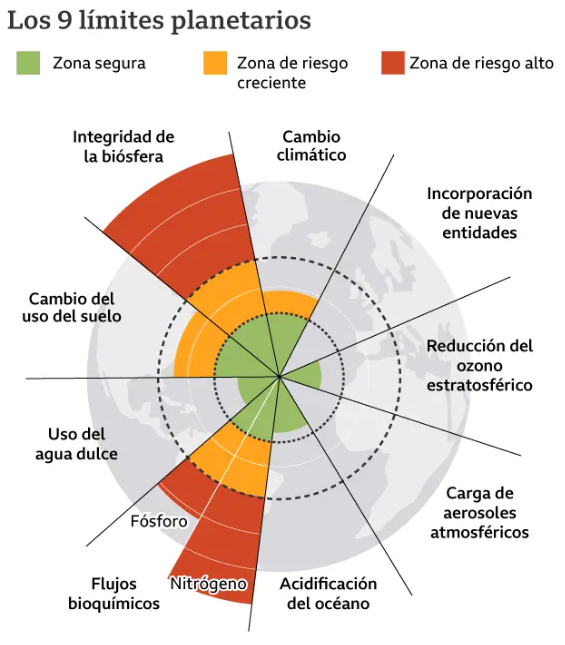
\includegraphics[width = 0.7\textwidth]{Imagenes/limitesplanetarios.png}
     	  	\captionof{figure}{\label{fig:limites}Los 9 limites planetarios \cite{IEEEreferencias:Ref2}.} 
    	   \end{center} 
        \end{figure}

 \subsection{Características típicas de aguas residuales textiles}    
 Antes de adentrarnos acerca de los catalizadores, es importante comenzar desde el problema que son los colorantes de tipo orgánico, ya que estos están formados por grupos de átomos llamados cromóforos. Estas moléculas se consideran importantes porque absorben selectivamente el color, para poder visualizarlo y distinguirlo ante el ojo humano \cite{Cromoforos}. Entre las moléculas que le dan ese color vibrante a los textiles se encuentran:\vspace{1em} % Espaciado adicional entre párrafos

\begin{itemize}
\item \textbf{Azo (-N=N-): } El cromóforo azo, se encuentra en los colorantes azoicos que son utilizados en la industria artificial o en pintura por la particularidad de su doble enlace entre los átomos de nitrógeno, es responsable de darle color a la R6G, ya que su característica principal es absorber la luz visible.
\item \textbf{Carbonilo (C=O): }Este grupo es el más importante en la química orgánica, se encuentra en tintes como las antraquinonas debido a la absorción de la luz a través de la resonancia del enlace carbono-oxígeno.
\item \textbf{Metilo (-$\displaystyle CH_{3}$):} aunque el grupo metilo en sí no es un cromóforo, pero dependiendo el número de metilos en la molécula, puede incrementar el tono y afectar la solubilidad del tinte.
\item \textbf{Nitro (-$\displaystyle NO_{2}$):} Los colorantes que contienen este grupo se caracterizan por ser muy brillantes y muy reactivos, por lo que se utilizan en determinadas aplicaciones industriales y a nivel laboratorio.
\item \textbf{Grupos quinoides:} estos grupos se encuentran comúnmente en tintes derivados de quinonas, como las antraquinonas, y son responsables de colores fuertes y estables que se implementan para repelentes, pinturas y medicamentos.
\end{itemize}
 
 \subsection{Colorantes}

 Entre los principales agravantes de la contaminación del agua se encuentran la industria azucarera, cervecera, de la destilería, del curtido, pulpa y papel y la más importante, la textil, que utiliza 120 m³/Ton de fibra con una concentración de color entre 1100 y 1300 en unidades Hazen de acuerdo con Adriana Cortazar et al \cite{IEEEreferencias:Ref3}.
\vspace{1em} % Espaciado adicional entre párrafos
 
 Por sus características se les considera peligrosos para la vida silvestre y los seres humanos, son causantes de enfermedades en altas concentraciones y de la eutrofización, que consiste en el crecimiento descontrolado de las algas en los ríos que impiden el paso de los rayos del sol a los cuerpos de agua, evitando la oxigenación del mismo y, en consecuencia, la muerte de la fauna acuática \cite{IEEEreferencias:Ref5}.
\vspace{1em} % Espaciado adicional entre párrafos

    \subsubsection{Xantenos}
    Entre la clasificación de los colorantes orgánicos, existen los xantenos, que se caracterizan por poseer una estructura molecular heterocíclica, con la capacidad de absorber la luz a una longitud de onda entre 570 y 590 nm, que le pertenece al color amarillo, razón de su fuerte fluorescencia. Se utiliza como detector molecular bajo el microscopio, cirugía láser y detección de pesticidas y fármacos \cite{IEEEreferencias:XANTENOS}. \vspace{1em} % Espaciado adicional entre párrafos
    
    La estructura molecular que poseen los xantenos está organizada por dos anillos de benceno conectados a través de un anillo de pirano central con un átomo de oxígeno, un ejemplo sería la eosina (Figura \ref{fig:eosina}) que tiene dos átomos de bromo conectados a cada benceno y dos moléculas de dióxido de nitrógeno.
     \begin{figure}[H]
    	   \begin{center}
     	  	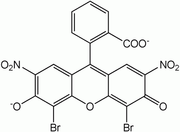
\includegraphics[width = 0.3\textwidth]{Imagenes/eosina.png}
     	  	\captionof{figure}{\label{fig:eosina}Molécula caracteristica de la eosina \cite{IEEEreferencias:Oxidacion}.} 
    	   \end{center} 
        \end{figure}
    \subsubsection{Rodaminas} 
    La rodamina de la molécula de la Figura \ref{fig:Rodamina}, es un tinte fluoróforo perteneciente a la familia de los colorantes orgánicos xantenos. Debido a su excelente fotoestabilidad y propiedades fotofísicas, la rodamina se puede utilizar en tintes láser, estándares fluorescentes, pigmentos fluorescentes y sondas para caracterizar la superficie, polimerización de nanopartículas poliméricas, detección de bioconjugados, estudios de adsorción de oligonucleótidos en látex, dinámica de micelas e imágenes de células vivas \cite{IEEEreferencias:XANTENOS}. \vspace{1em} % Espaciado adicional entre párrafos
    
    Dependiendo de los sustituyentes G, R1, R2, R3, R4 e incluso los contraiones (generalmente) en su estructura molecular, los tintes exhibirán diferentes propiedades fotofísicas en solución, como diferentes máximos de absorción y emisión, tiempos de fluorescencia y rendimiento cuántico de fluorescencia \cite{IEEEreferencias:XANTENOS}.

\begin{figure}[H]
    	   \begin{center}
     	  	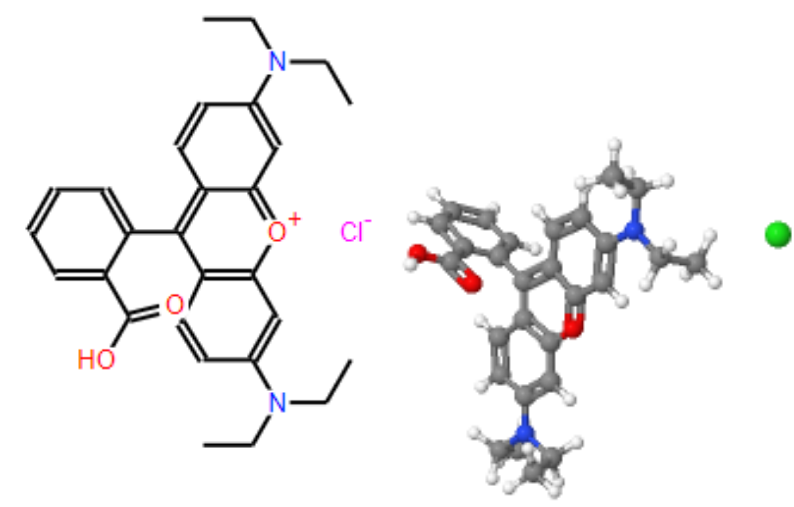
\includegraphics[width = 0.4\textwidth]{Imagenes/Rodamina_Molecula (2).png}
     	  	\captionof{figure}{\label{fig:Rodamina}Molécula característica de las rodaminas . La figura se obtuvo de biomodel.uah.es y de \cite{herraez-no-date}.}
            \end{center} 
        \end{figure}

 
    \subsubsection{Rodamina 6G}


La Rodamina 6G (R6G) con estructura molecular de la Figura \ref{fig:R6G_MOLECULAS}, es un colorante fluorescente ampliamente utilizado en aplicaciones industriales, de laboratorio y como trazador en estudios de flujo de agua. Su liberación en el medio ambiente, especialmente en cuerpos de agua, es motivo de preocupación debido a su estabilidad química y potencial bioacumulativo.\vspace{1em} % Espaciado adicional entre párrafos 

La R6G puede persistir en el agua durante largos períodos, y las concentraciones que se encuentran comúnmente en aguas residuales industriales oscilan entre 0.01 y 1 mg/L. Aunque parece ser una concentración baja, incluso pequeñas cantidades de R6G pueden impactar negativamente los ecosistemas acuáticos al afectar la fotosíntesis de las plantas acuáticas y la calidad del agua \cite{IEEEreferencias:Ref11}.\vspace{1em} % Espaciado adicional entre párrafos

La Rodamina 6G es conocida por su toxicidad en organismos acuáticos. La exposición a concentraciones superiores a 0.1 mg/L puede resultar en efectos adversos para organismos como peces, algas y bacterias. La R6G puede inducir daño celular al generar especies reactivas de oxígeno (ROS), lo que lleva a \'{e}str\'es oxidativos y daño en las membranas celulares.\vspace{1em} % Espaciado adicional entre párrafos 

En humanos, la R6G es considerada un posible carcin\'ogeno, y la exposición prolongada o en altas concentraciones puede resultar en irritaci\'on de la piel y las v\'ias respiratorias, así como posibles daños hep\'aticos y renales. Aunque su uso en aplicaciones m\'edicas es limitado, la exposición accidental a altas dosis puede presentar riesgos para la salud.\vspace{1em} % Espaciado adicional entre párrafos

\begin{figure}[H]
    	   \begin{center}
     	  	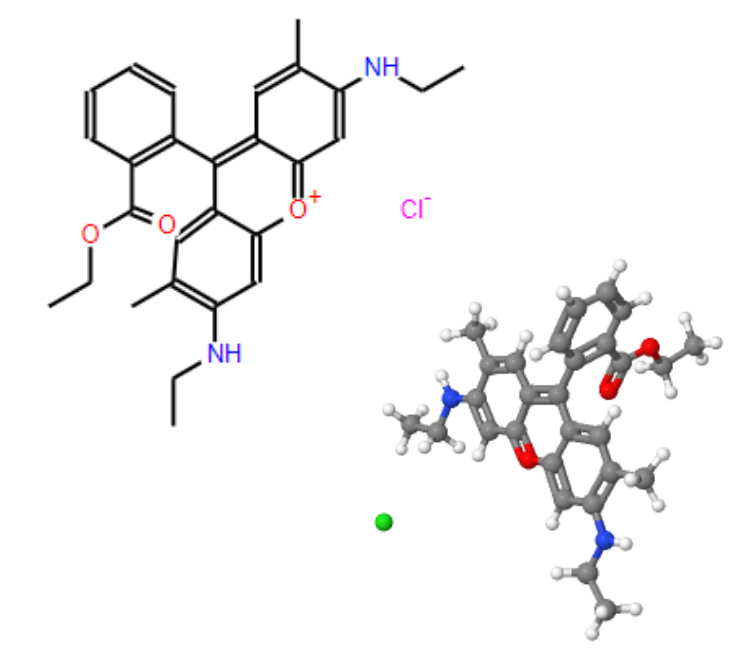
\includegraphics[width = 0.4\textwidth]{Imagenes/R6G_MOLECULAS.png}
     	  	\captionof{figure}{\label{fig:R6G_MOLECULAS}Estructura molecular de la R6G de metileno, colorante de la familia de los xantenos, formado por dos cromóforos, un grupo dibenzopireno y un grupo carboxifenilo \cite{herraez-no-date}.} 
    	   \end{center} 
        \end{figure}
    \subsubsection{Triarimetano}
     Los colorantes orgánicos del grupo de los triarimetano se utilizan para la fabricación de tinta que absorbe la luz a una longitud de onda entre 380 y 500 nm que es característica del color azul. En la industria se utiliza para darle ese color vibrante al papel, tintas de impresión, de pastas para bolígrafos, etc. Bajo el término de “Azul Victoria” se conoce un grupo de colorantes de triarilmetano catiónicos, que contienen un resto naftilo sustituido por alquilamino y/o por arilamino\cite{IEEEreferencias:AM_1}. Están formados por tres bencenos, como se ilustra en la Figura \ref{fig:triarimetano}.
     \begin{figure}[H]
    	   \begin{center}
     	  	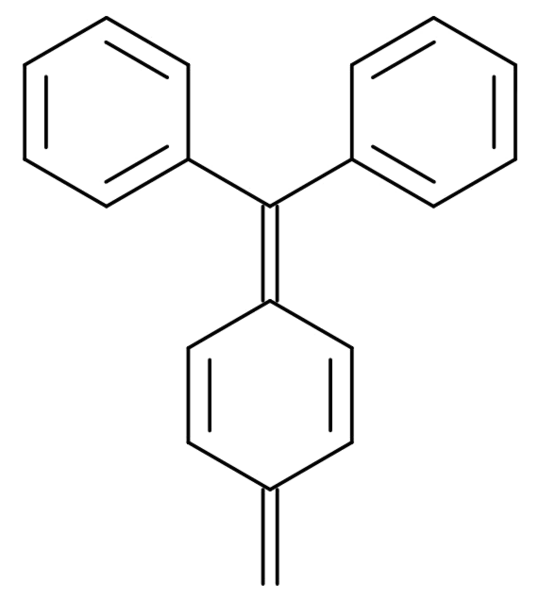
\includegraphics[width = 0.2\textwidth]{Imagenes/triarimetano.png}
     	  	\captionof{figure}{\label{fig:triarimetano}Molécula de triarimetano \cite{herraez-no-date}.}
    	   \end{center} 
        \end{figure}
     
  \subsubsection{Azul de Metileno}
    El azul de metileno, con estructura molecular de la Figura \ref{fig:BM_MOLECULA}, es un compuesto químico que se utiliza en una variedad de aplicaciones, incluyendo la industria química, la microbiología, la medicina y la tintura de tejidos \cite{IEEEreferencias:AM_1}. 

    Es importante destacar que el uso de azul de metileno debe llevarse a cabo con precaución y siguiendo las pautas de seguridad adecuadas, ya que es una sustancia química y puede tener efectos adversos en la salud si se maneja de manera inapropiada. Además, las investigaciones sobre sus posibles aplicaciones médicas siguen siendo objeto de estudio y desarrollo \cite{IEEEreferencias:AM_1}.\vspace{1em} % Espaciado adicional entre párrafos 

    Los estudios han demostrado que concentraciones de AM tan bajas como 0.1 a 1 mg/L pueden ser tóxicas para ciertos organismos acuáticos, como peces y algas. Estas concentraciones pueden causar alteraciones en la respiración y la función celular, además de afectar la capacidad fotosintética de las plantas acuáticas.\vspace{1em} % Espaciado adicional entre párrafos

     Las dosis terapéuticas en medicina suelen ser seguras y oscilan entre 1-2 mg/kg de peso corporal. Sin embargo, una sobredosis o exposición accidental a cantidades superiores puede resultar en efectos adversos como metahemoglobinemia, que afecta la capacidad de la sangre para transportar oxígeno.\vspace{1em} % Espaciado adicional entre párrafos


    La exposición dérmica o inhalatoria al polvo o a soluciones concentradas puede causar irritación, y la ingestión de cantidades superiores a 7 mg/kg puede ser peligrosa, llevando a síntomas como náuseas, vómitos y mareos.\vspace{1em} % Espaciado adicional entre párrafos

\begin{figure}[H]
    	   \begin{center}
     	  	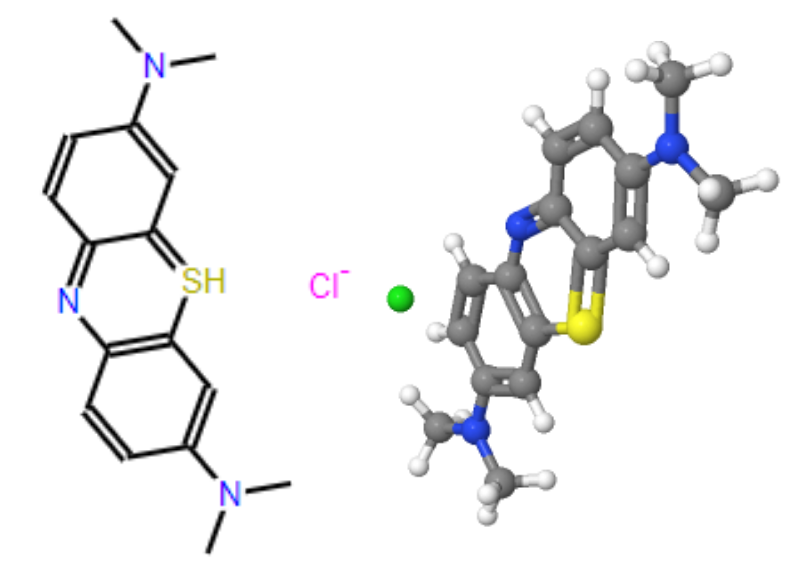
\includegraphics[width = 0.4\textwidth]{Imagenes/BM_MOLECULA.png}
     	  	\captionof{figure}{\label{fig:BM_MOLECULA}Estructura molecular del azul de metileno, colorante perteneciente a la familia de los trifenilmetano, formada por un compuesto aromático, dos aminas y cuatro metileno \cite{herraez-no-date}.}
    	   \end{center} 
        \end{figure}

 \subsection{Métodos para degradar colorantes}

Los colorantes industriales son compuestos orgánicos que se utilizan ampliamente en diversas industrias, como la textil, papelera, alimentaria y cosmética. Sin embargo, la liberación de estos colorantes en cuerpos de agua puede causar contaminación significativa debido a su naturaleza tóxica y resistencia a la degradación. Por lo tanto, es crucial desarrollar y aplicar métodos eficaces para la degradación de estos compuestos.\vspace{1em} % Espaciado adicional entre párrafos
Como se ilustra en la Figura \ref{fig:MetodosDegradación} algunas de las tecnologías que existen para combatir los efluentes en los cuerpos de agua, desde los físicos, químicos, biológicos, electroquímicos y en los que nos vamos a enfocar, que son los métodos de Oxidación Avanzada  \cite{IEEEreferencias:OxiA1,IEEEreferencias:OxiA2,IEEEreferencias:OxiA3, IEEEreferencias:Oxidacion}.\vspace{1em} % Espaciado adicional entre párrafos

Cada uno cuenta con sus ventajas y desventajas, pero elegiremos la Oxidación Avanzada porque a partir de la energía de la luz UV del medio, es posible descomponer los cromóforos de colorantes como R6G y AM.

\begin{figure}[H]
    	   \begin{center}
     	  	\includegraphics[width = 1\textwidth]{Imagenes/MetodosDegradación.png}
     	  	\captionof{figure}{\label{fig:MetodosDegradación}Metodos de degradación.} 
    	   \end{center} 
        \end{figure}


 \subsection{Tipos de procesos de oxidación avanzada} 

 Las tecnologías que intervienen en la calidad del agua a través de la adsorción, la coagulación y la separación por membranas, son técnicas, que solo tienen la capacidad de concentrar o transformar los contaminantes orgánicos recalcitrantes en la fase sólida constituyente del agua. Por lo tanto, es inevitable la implementación de tratamientos adicionales para transformar los contaminantes secundarios persistentes y activar el proceso de regeneración de los adsorbentes que requieren costo adicional \cite{IEEEreferencias:Ref5}.
\vspace{1em} % Espaciado adicional entre párrafos

Cada método tiene sus propias ventajas y desventajas, y la elección del método adecuado depende de factores como el tipo de colorante, la concentración de contaminantes, el costo y las regulaciones ambientales. Los métodos de oxidación avanzada, aunque pueden ser más costosos, ofrecen una gran eficiencia en la degradación de colorantes debido a la capacidad de los radicales libres para atacar y descomponer una amplia gama de contaminantes orgánicos. Estos se clasifican en procesos homogéneos y heterogéneos con dos subcategorías de no fotoquímicos y fotoquímicos, como se ilustra en el diagrama de la Figura \ref{fig:TiposDeOxidacion}.
 \begin{figure}[H]
    	   \begin{center}
     	  	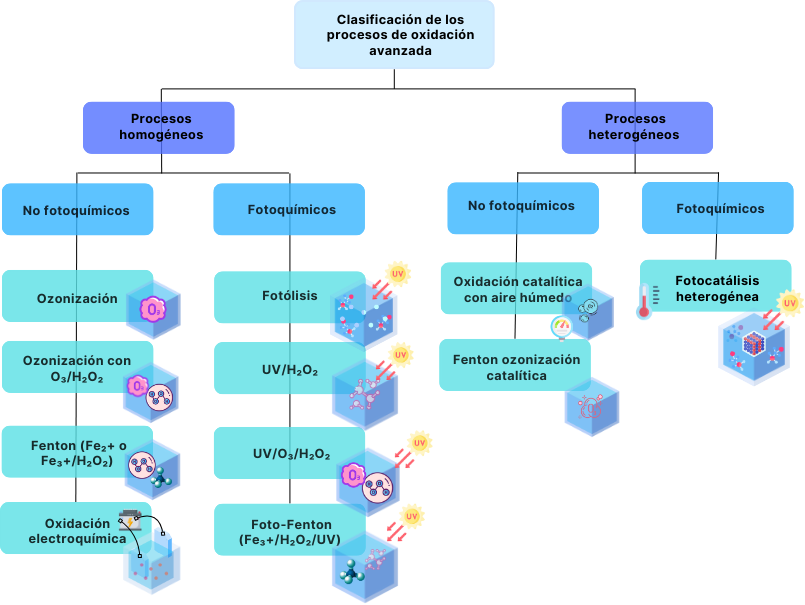
\includegraphics[width = 0.9\textwidth]{Imagenes/TiposDeOxidacion (2).png}
     	  	\captionof{figure}{\label{fig:TiposDeOxidacion}Diagrama de tipos de Oxidación Avanzada.} 
    	   \end{center} 
        \end{figure}
 \subsection{Fotocatálisis heterogénea }
 La fotocatálisis (Figura \ref{fig:FOTOCATALISIS}) es un proceso de adsorción, donde especies reactivas se unen a la superficie del fotocatalizador; es esencial para la activación de reacciones químicas. Los sitios activos en la superficie del fotocatalizador actúan como centros de adsorción, facilitando la interacción entre reactantes y promoviendo la formación de complejos reactivos \cite{IEEEreferencias:Ref6, IEEEreferencias:Ref10}.
\vspace{1em} % Espaciado adicional entre párrafos

Las reacciones subsiguientes, gobernadas por la cinética de reacción y barreras energéticas, determinan la eficiencia y selectividad del proceso fotocatalítico. En el mecanismo de Langmuir-Hinshelwood, estas reacciones son típicamente de primer orden o pseudo-primer orden. La cinética de reacción se ha analizado detalladamente mediante técnicas de seguimiento, espectroscopía y electroquímica \cite{IEEEreferencias:Ref7}. 
\vspace{1em} % Espaciado adicional entre párrafos

La desorción de productos es un paso crucial que regenera los sitios activos para iniciar nuevas reacciones. La eficiencia de la desorción se ve influenciada por factores como la temperatura, presión y la naturaleza de las especies adsorbidas y productos formados. Estudios teóricos y experimentales han proporcionado entendimiento sobre la termodinámica de la desorción y su impacto en la eficiencia global de la fotocatálisis \cite{IEEEreferencias:Ref8}. 
\vspace{1em} % Espaciado adicional entre párrafos

     \begin{figure}[H]
        	\begin{center}
         		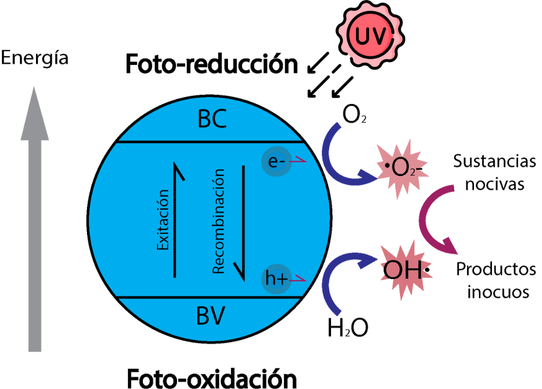
\includegraphics[width = 0.7\textwidth]{Imagenes/FOTOCATALISIS.png}
         		\caption{Imagen que describe el proceso de la fotocatálisis al convertir la energía solar en energía química.}
           \label{fig:FOTOCATALISIS} 
           
        	\end{center} 
        \end{figure}
 \subsubsection{Métodos de fotocatalisis}
 \subsubsubsection{Mecanismo de Langmuir-Hinshelwood}\vspace{1em}
 
 La adsorción inicial de especies reactivas en la superficie del fotocatalizador emerge como un paso crucial para activar reacciones químicas. Los sitios activos en la superficie del fotocatalizador actúan como centros de absorción para especies reactivas en fase líquida o gaseosa. El escrutinio de este proceso de adsorción implica técnicas experimentales sofisticadas como la espectroscópia infrarroja y la microscopía de fuerza atómica, proporcionando detalles intrincados sobre la naturaleza de los enlaces formados entre las especies y la superficie del fotocatalizador \cite{IEEEreferencias:Ref10}.\vspace{1em} % Espaciado adicional entre párrafos 

Las subsiguientes reacciones entre las especies adsorbidas están dictadas por la cinética de reacción y las barreras energéticas inherentes en cada etapa del proceso. En el mecanismo de Langmuir-Hinshelwood (Figura \ref{fig:MetodosFotocatalisis}), estas reacciones generalmente exhiben cinética de primer orden o pseudo-primer orden, dicho de otra forma, la concentración de una de las especies reactivas es responsable de la velocidad de reacción. La cinética de reacción, examinada a través de métodos como el seguimiento de reacciones, la espectroscópia de absorción y técnicas electroquímicas, desempeña un papel crucial en determinar la eficiencia y selectividad del proceso fotocatalítico \cite{IEEEreferencias:Ref10}. \vspace{1em} % Espaciado adicional entre párrafos

Crucialmente, la desorción de productos culmina el mecanismo de Langmuir-Hinshelwood, rejuveneciendo los sitios activos en la superficie del fotocatalizador para iniciar nuevas reacciones. La eficacia de la desorción se ve influenciada por parámetros como la temperatura, la presión y la naturaleza de las especies adsorbidas y los productos formados. Estudios teóricos y experimentales han desentrañado la termodinámica de la desorción, elucidando su impacto en la eficiencia global de la fotocatálisis \cite{IEEEreferencias:Ref10}.\vspace{1em} % Espaciado adicional entre párrafos 

En resumen, el mecanismo de Langmuir-Hinshelwood gobierna intrincadamente la fotocatálisis heterogénea, dirigiendo la adsorción de especies reactivas, las subsiguientes reacciones entre especies adsorbidas y la desorción de productos. Este mecanismo, sujeto a una exploración extensiva en la literatura científica mediante técnicas experimentales y estudios teóricos, proporciona una comprensión profunda de los factores que dictan la eficiencia y selectividad en la fotocatálisis \cite{IEEEreferencias:Ref10}. 
\begin{figure}[H]
    	   \begin{center}
     	  	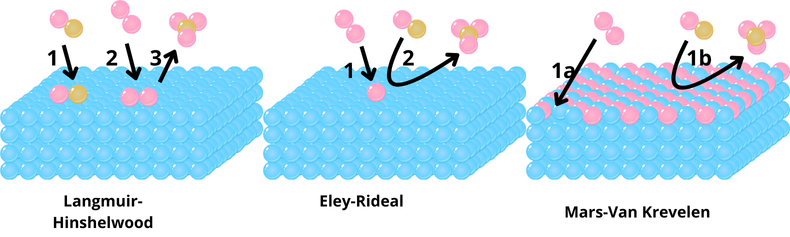
\includegraphics[width = 1\textwidth]{Imagenes/MetodosFotocatalisis.png}
     	  	\captionof{figure}{\label{fig:MetodosFotocatalisis}Pruebas en oscuro y con lampara UV de la R6G\cite{phdthesis,article_1}.} 
    	   \end{center} 
        \end{figure}
\subsection{Nanotecnología}
    La nanotecnología es la parte de los nanomateriales que se enfoca en poner en práctica las propiedades de los nanomateriales, es muy diferente lo que ocurre a nivel experimental en el laboratorio que a nivel industrial, es decir, al incrementar el tamaño de las partículas su morfología cambia y en consecuencia también cambian sus características eléctricas, ópticas, magnéticas. Es un proceso muy complicado por estar en pleno desarrollo, pero está en constante evolución por todas las investigaciones que se están llevando a cabo.\cite{IEEEreferencias:Ref1}
    \subsection{Nanociencia}
    La nanociencia junto con la nanotecnología son dos temas nuevos en la ciencia de los materiales, debido a que nos dan la oportunidad de investigar los fenómenos que a simple vista serían imperceptibles al ojo humano, ya que solo se presenta en tamaño molecular. Lo interesante de la nanociencia es que a escala nanométrica los materiales tienen capacidades diferentes a las que tienen a escala macroscópica, lo que los hace muy importantes en la industria de la electrónica para fabricar componentes cada vez más pequeños y ahorrar en material \cite{IEEEreferencias:Ref1}.
    \subsection{Nanomateriales}
    Desde el punto de vista de la nano escala, los nanomateriales son materiales que contienen partículas con una o más dimensiones, en otras palabras, 1 nm = 10-9 m. Gracias a que es posible cambiar sus propiedades a partir de la modificación de parámetros de síntesis, se pueden utilizan en la ingeniería, la medicina, la electrónica, la biología. Los nanomateriales se dividen de acuerdo a su tamaño, existen entre 0-D, 1-D, 2-D, 3-D, que se muestran a continuación en la Figura \ref{fig:Nanomateriales_ imagen} \cite{IEEEreferencias:Ref9,IEEEreferencias:NANO1, IEEEreferencias:NANO2}.
    
     
\begin{figure}[H]
        	\begin{center}
         		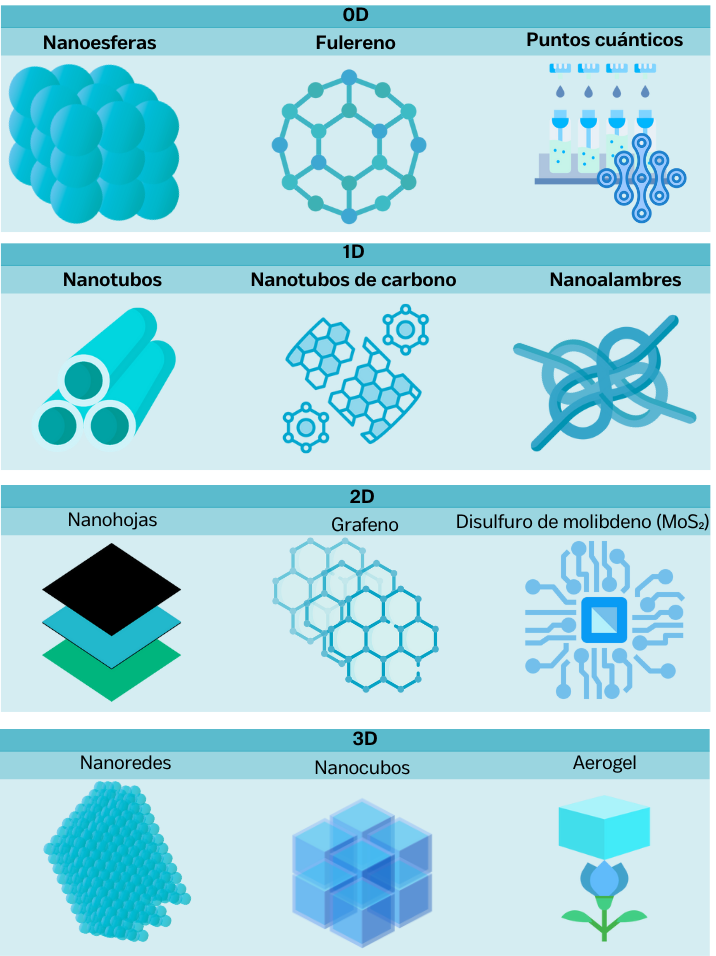
\includegraphics[width = 0.9\textwidth]{Imagenes/Nanomateriales_ imagen.png}
         		\caption{Clasificación de nanomateriales, imagen obtenida de \cite{IEEEreferencias:NANO2}.}
           \label{fig:Nanomateriales_ imagen} 
           
        	\end{center} 
        \end{figure}


     
     \subsubsection{Nanomateriales a base de carbono (CNT)}
     Los nanomateriales a base de carbono que forman parte de la Figura \ref{fig:Nanomateriales_ imagen}, como los fulerenos, nanotubos de carbono (CNT), grafeno y óxido de grafeno, este último es de interés para esta investigación. Están compuestos por láminas de grafito enrolladas en forma de tubos, lo que les confiere propiedades únicas y diversas aplicaciones en diversos campos.\vspace{1em} % Espaciado adicional entre párrafos


    Sin embargo, también hay desafíos asociados con los nanotubos de carbono, como la dificultad de producción a gran escala, la dispersión y alineación controlada, la eliminación de impurezas y la gestión de riesgos para la salud y el medio ambiente debido a su forma y tamaño nanoestructurado. Estos aspectos deben ser considerados y abordados para aprovechar plenamente el potencial de los nanotubos de carbono en diversas aplicaciones \cite{IEEEreferencias:GO_8,IEEEreferencias:GO_GOr}.

    \subsubsection{Nanomateriales semiconductoras}
    Los nanomateriales se pueden clasificar no solo por su tamaño, sino también debido a sus propiedades como conductores, aislantes y semiconductores (Figura \ref{fig:SeminCondAisl}), estos últimos exhiben un cambio en el tamaño de banda de energía debido a su tamaño de reducido lo que permite que al ser sus electrones exitados puedan actuar como condutores o como aislantes. Esto significa que sus propiedades ópticas y electrónicas pueden ser ajustadas mediante el control del tamaño de partícula. Esta flexibilidad permite el diseño de materiales con propiedades específicas para diversas aplicaciones.\vspace{1em} % Espaciado adicional entre párrafos

    Los nanomateriales semiconductores encuentran aplicaciones en una amplia gama de campos, como la electrónica, la optoelectrónica, la energía fotovoltaica, la catálisis, la medicina y la ciencia de los materiales. Sin embargo, también existen desafíos asociados con la síntesis, estabilidad y toxicidad de los nanomateriales semiconductores, lo que requiere una consideración cuidadosa de su fabricación y manipulación.
\begin{figure}[H]
    	   \begin{center}
     	  	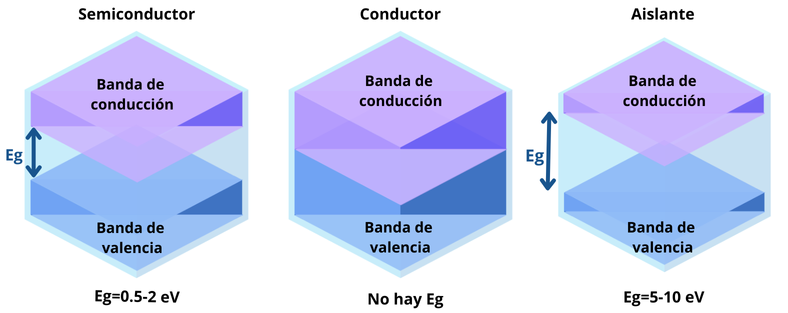
\includegraphics[width = 1\textwidth]{Imagenes/SeminCondAisl.png}
     	  	\caption{Banda ancha de los nanomateriales. }\label{fig:SeminCondAisl}  
    	   \end{center} 
        \end{figure}

    \subsection{Materiales fotocatalizadores convencionales}
    La fotocatálisis es una tecnología prometedora como uno de los métodos de oxidación avanzada. Para poner en práctica este procedimiento de degradación de contaminantes es indispensable un catalizador, pero que pasa si combinamos un semiconductor con GO. En esta investigación utilizaremos el dióxido de estaño (SnO$\displaystyle _{2}$) y el óxido de zinc (ZnO) para decorar el óxido de grafeno (GO. \vspace{1em} % Espaciado adicional entre párrafos
    
    El SnO$\displaystyle _{2}$  y el ZnO son semiconductores que presentan una banda ancha de 3.6, 3.37 eV respectivamente. Esto es de suma importancia, ya que una banda prohibida pequeña nos permite absorber luz en la región visible, ampliando su eficiencia bajo luz solar. El efecto que produce es excitar electrones con luz UV desde la banda de valencia a la banda de conducción, dejando huecos en la banda de valencia, que van a producir una reacción redox ante el colorante.\vspace{1em} % Espaciado adicional entre párrafos

    La reacción redox se efectúa por parte de los electrones en la banda de conducción, al generar radicales superóxidos. La banda de valencia forma huecos y reacciones de oxidación, como la formación de radicales hidroxilo.\vspace{1em} % Espaciado adicional entre párrafos
    
    \subsubsection{Óxido de grafeno}
    El óxido de grafeno o GO (Figura \ref{fig:Grafeno_dibujo}), es un material alotrópico (tiene varias formas) que comparte la estructura del grafeno junto con grupos funcionales de oxígeno. Las aplicaciones dependen del grado de oxidación del grafeno. El GO es un material con propiedades hidrofílicas (repele el agua y puede formar coloides acuosos estables), cuenta con un área superficial amplia, es ideal para combinar con polímeros y otros materiales como el ZnO y el SnO$\displaystyle_{2}$ en este caso. Las aplicaciones que tiene el GO en la industria normalmente se utilizan en plásticos, recubrimientos anticorrosivos, recubrimientos antimicrobianos, reforzamiento de construcción y para empaques \cite{IEEEreferencias:Ref12,IEEEreferencias:GO_1}.

    \begin{figure}[H]
    	   \begin{center}
     	  	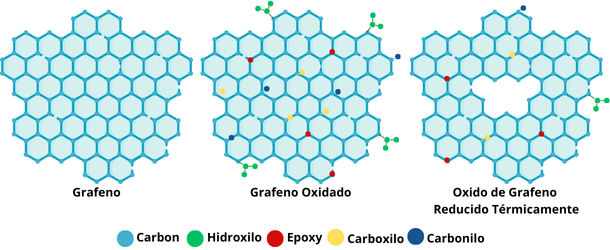
\includegraphics[width = 1\textwidth]{Imagenes/Grafeno_dibujo.png}
     	  	\caption{a) Estructuras de grafeno, GO y TrGO; b) obtención de TrGO a partir
de grafeno \cite{IEEEreferencias:GO_GOr}. }\label{fig:Grafeno_dibujo}  
    	   \end{center} 
        \end{figure}

        
    \subsubsection{Dióxido de Estaño}
    El SnO$\displaystyle _{2}$ tiene estructura de rutilo y cristaliza en el grupo espacial tetragonal P4$\displaystyle _{2}$/mnm. El Sn⁴⁺ está unido a seis átomos equivalentes de O²⁻ para formar una mezcla de octaedros de SnO$\displaystyle _{6}$ que comparten esquinas y bordes. Los ángulos de inclinación octaédricos que comparten esquinas son 51°. Hay dos longitudes de enlace Sn-O más cortas (2,06 Å) y cuatro más largas (2,07 Å). El O²⁻ está unido en una geometría plana trigonal a tres átomos de Sn⁴⁺ equivalentes.\vspace{1em} % Espaciado adicional entre párrafos
    
    El dióxido de estaño (SnO$\displaystyle _{2}$) es un material semiconductor tipo n con una estructura cristalina tetragonal centrada en las caras, conocida como estructura de rutilo (Figura \ref{fig:Rutilo}) y es la más común y estable para el SnO$\displaystyle _{2}$ a condiciones de temperatura ambiente. Es un sólido cristalino, con importantes características ópticas, electrónicas y químicas, que le permiten reaccionar con ácidos para la elaboración de otros compuestos de estaño, acabados de contactos eléctricos, el estañado de utensilios de cocina; es un material útil para la elaboración de sensores de gas, varistores, catalizadores, dispositivos optoeléctricos, fotocatalizadores. La energía es un importante elemento para la elaboración de paneles fotovoltaicos, los cuales se utilizan para producir electricidad a partir de la luz solar.\vspace{1em} % Espaciado adicional entre párrafos

El SnO$\displaystyle _{2}$  tiene características como ser transparente a la luz visible, un material tipo n que cuenta con una alta conductividad eléctrica cuando se dopa con impurezas donadoras, estabilidad química y baja toxicidad que lo convierten en un material de interés en la investigación y desarrollo de nuevos dispositivos y tecnologías\cite{IEEEreferencias:Ref10,IEEEreferencias:Ref11,IEEEreferencias:Ref12,IEEEreferencias:Ref13,IEEEreferencias:Ref14,IEEEreferencias:Ref15, IEEEreferencias:Ref16, IEEEreferencias:Ref17}.

        \begin{figure}[H]
    	   \begin{center}
     	  	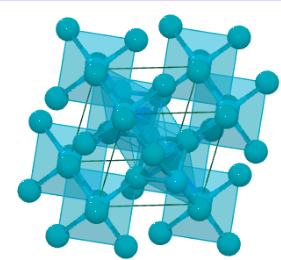
\includegraphics[width = 0.5\textwidth]{Imagenes/Rutilo.png}
     	  	\caption{Estructura cristalino de rutilo en el SnO$\displaystyle _{2}$.}\label{fig:Rutilo}  
    	   \end{center} 
        \end{figure}
     
    \subsubsection{Óxido de Zinc}
    El óxido de zinc (ZnO) es un material semiconductor, cuenta con una alta conductividad eléctrica, una alta transmisión óptica en el visible, una alta reflectancia en el infrarrojo, cuenta con una buena estabilidad térmica y química, su estructura cristalina es Wurtzita (Figura \ref{fig:ZnO_Cristal}). El ZnO tiene aplicaciones en la optoeléctrica para la fabricación de láseres en la longitud de onda ultravioleta, es un material con la capacidad de mejorar la grabación y sustituir al LED, HD-DVD y Blue Ray. Otras aplicaciones importantes de este material es la fabricación de celdas solares, para los dispositivos piezoeléctricos, en sustratos heteroepitaxias, la manufactura de pinturas, en los cosméticos y en productos farmacéuticos \cite{IEEEreferencias:Ref13,IEEEreferencias:ZnO1, IEEEreferencias:ZnO2, IEEEreferencias:ZnO3,IEEEreferencias:ZnO4, IEEEreferencias:ZnO5,IEEEreferencias:ZnO6, IEEEreferencias:ZnO7, IEEEreferencias:ZnO8,IEEEreferencias:ZnO9, IEEEreferencias:ZnO10, IEEEreferencias:ZnOGO_Fotocatalisis_2,IEEEreferencias:ZnOGO_Fotocatalisis_3,IEEEreferencias:ZnOGO_Fotocatalisis_4, IEEEreferencias:ZnOGO_Fotocatalisis_5, IEEEreferencias:ZnOGO_Fotocatalisis_6, IEEEreferencias:ZnOGO_Fotocatalisis_7}.
    
        \begin{figure}[H]
    	   \begin{center}
     	  	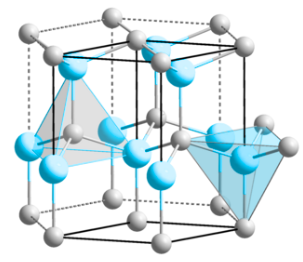
\includegraphics[width = 0.5\textwidth]{Imagenes/ZnO_Cristal.png}
     	  	\caption{Estructura cristalino de rutilo en el ZnO.}\label{fig:ZnO_Cristal}  
    	   \end{center} 
        \end{figure}
     

    
    \subsection{Síntesis de nanomateriales}
    La síntesis de nanomateriales se refiere al proceso de fabricación y producción de materiales en una escala nanométrica, es decir, a nivel de nanómetros (1 nanómetro equivale a una milmillonésima parte de un metro). Hay dos enfoques principales utilizados en la síntesis de nanomateriales: el enfoque "Top-Down" (de arriba hacia abajo) y el enfoque "Bottom-Up" (de abajo hacia arriba) (Figura \ref{fig:Metodos de Sintesis}). Ambos enfoques tienen diferencias en términos de su enfoque y métodos de fabricación \cite{IEEEreferencias:TOPDOWN_BOTTOMUP}.
        \subsubsection{Top-Down}
        Desde el punto de vista de Top-Down, los nanomateriales se sintetizan reduciendo el tamaño de una estructura más grande hasta llegar a la escala nanométrica, desde lo general a lo específico. Implica la modificación y manipulación de materiales de mayor tamaño para obtener nanoestructuras. Algunos métodos comunes utilizados en el enfoque Top-Down incluyen la litografía, la molienda de alta energía y la ablación láser. Este enfoque permite un control preciso sobre la forma y tamaño de los nanomateriales, pero puede tener limitaciones en términos de la uniformidad y la escala de producción \cite{IEEEreferencias:TOPDOWN_BOTTOMUP}.
        
        \subsubsection{Bottom-up}
    En este enfoque, los nanomateriales se sintetizan a partir de componentes más pequeños, como átomos, moléculas o iones, que se ensamblan gradualmente para formar nanoestructuras más grandes. Se utilizan reacciones químicas y métodos de autoensamblaje para construir los nanomateriales.\vspace{1em} % Espaciado adicional entre párrafos
    
    Ejemplos de métodos Bottom-Up incluyen la síntesis hidrotermal, la precipitación química, la deposición de vapor químico y la autocatálisis. Este enfoque permite una mayor flexibilidad en la composición y estructura de los nanomateriales, pero puede requerir condiciones de síntesis más controladas y puede ser más difícil de escalar a niveles de producción masiva \cite{IEEEreferencias:TOPDOWN_BOTTOMUP}.
\vspace{1em} % Espaciado adicional entre párrafos
    
    Tanto el enfoque Top-Down como el Bottom-Up tienen sus propias ventajas y desafíos, y su elección depende de los requisitos específicos de la aplicación y las propiedades deseadas de los nanomateriales. Ambos enfoques juegan un papel importante en la síntesis y aplicación de nanomateriales en diversos campos, como la electrónica, la medicina, la energía y la ciencia de los materiales.
    \begin{figure}[H]
    	   \begin{center}
     	  	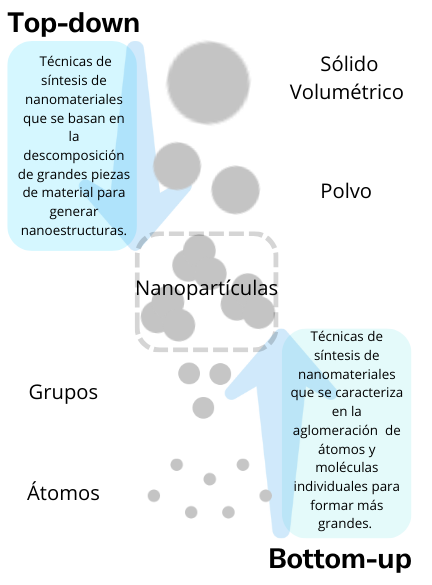
\includegraphics[width = 0.5\textwidth]{Imagenes/Metodos de Sintesis.png}
     	  	\caption{Métodos de síntesis\cite{IEEEreferencias:TOPDOWN_BOTTOMUP_1}.}\label{fig:Metodos de Sintesis}  
    	   \end{center} 
        \end{figure}
     

        \subsubsection{Método Hidrotermal}
           El método hidrotermal ha aportado a la investigación científica en campos como los materiales, metalurgia, física, química, biológica, electrónica, etc.  En la parte de los materiales semiconductores se experimenta a partir de controlar la calidad ajustando la proporción de materiales de partida (precursor y reductor), el pH del sistema de reacción, tiempo y temperatura de reacción \cite{IEEEreferencias:Ref10}.\vspace{1em} % Espaciado adicional entre párrafos
        
        El método hidrotermal (Figura \ref{fig:hidrotermal}) consiste en el uso de una solución acuosa como sistema de reacción en un recipiente de reacción cerrado especial para crear un ambiente de reacción a una alta presión y temperatura, calentando el sistema de reacción y presurizándolo. El proceso disuelve y recristaliza sustancias poco solubles o insolubles bajo condiciones normales \cite{IEEEreferencias:Ref10}.\vspace{1em} % Espaciado adicional entre párrafos        


         \begin{figure}[H]
    	   \begin{center}
     	  	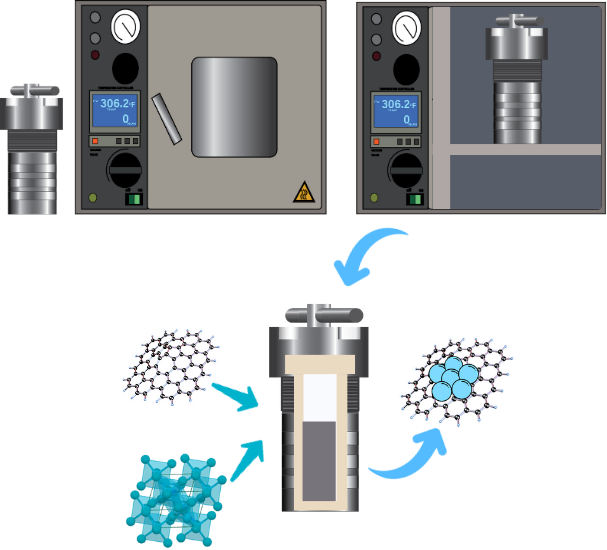
\includegraphics[width = 0.6\textwidth]{Imagenes/hidrotermal.png}
     	  	\caption{Proceso de la síntesis hidrotermal.}\label{fig:hidrotermal}  
    	   \end{center} 
        \end{figure}
     
        
        
        \subsubsection{Método de Hummer}
        El método de Hummers es un proceso químico, seguro, rápido y eficiente que se utiliza para sintetizar el óxido de grafeno mediante la adición de permanganato de potasio a una solución de grafito, nitrato de sodio y ácido sulfúrico. Es comúnmente utilizado por ingenieros y técnicos de laboratorio como un método confiable para producir cantidades de óxido de grafeno. Existen otros métodos para la obtención de GO por ejemplo, el método de Staudenmeier-Hoffman-Hamdi, pero este tiene la desventaja de ser más peligroso por la implementación del clorato de potasio.\cite{IEEEreferencias:Ref1}
        
    \subsection{Técnicas de caracterización}
    La espectroscopia tiene como objetivo estudiar las características de la materia, ya sea cualitativa o cuantitativa; se originó como el estudio de la interacción entre radiación y materia en función de la longitud de onda. En los últimos años, los materiales formados por carbono han tenido un gran impacto en la medicina, electrónica, energía y en el área de nanomateriales.\vspace{1em} % Espaciado adicional entre párrafos      
    
    Debido a las propiedades del SnO$\displaystyle _{2}$, ZnO y el óxido de grafeno, por ser potenciales materiales para efectuar la fotocatálisis, debido a sus caracteristicas oxidantes, se utilizan técnicas de caracterización para identificar sus propiedades y explicar a partir de equipos especializados el comportamiento, fiabilidad, absorbancia y posibles aplicaciones.\vspace{1em} % Espaciado adicional entre párrafos      
    
    Las técnicas que utilizaremos para describir nuestros catalizadores son: la microscopia electrónica de barrido (SEM), la espectroscopia de RAMAN, espectroscopia infrarroja por transformada de Fourier (FTIR), espectroscopia ultravioleta-visible (UV-VIS), espectroscopía fotoelectrónica de rayos X (XPS) y la difracción de rayos X (DRX) \cite{IEEEreferencias:Ref15}.
    
        \subsubsection{Difracción de Rayos X (XRD)}
        La difracción de rayos X (XRD) es la técnica de caracterización más potente para estudiar la estructura de cristales. Por ser los fotones partículas de masa en reposo y libres de carga, cuando estos se dispersan como un haz de rayos X, interactúan con la materia de manera no violenta, por lo tanto, la muestra no requiere un tratamiento o cubrimiento especial para ser caracterizada como se ilustra en la Figura \ref{fig:DRX_1} \cite{IEEEreferencias:Ref17}.\vspace{1em} % Espaciado adicional entre párrafos     

        El resultado es un patrón de puntos en una placa o detector, donde cada punto representa la intensidad de los rayos X difractados en un ángulo específico, como una huella dactilar que posee cada elemento y con la que se puede identificar si se sintetizó el material puro o con defectos.\vspace{1em} % Espaciado adicional entre párrafos     
        
        Este ángulo específico se le conoce como los ángulos de Bragg, los cuales están relacionados con la distancia entre los planos atómicos en el cristal y la longitud de onda de los rayos X utilizados en el experimento mediante la Ley de Bragg de la ecuación~\ref{eq:1} y \ref{eq:2} \cite{IEEEreferencias:Bragg}.\vspace{1em} % Espaciado adicional entre párrafos     

        \begin{gather}
        n\lambda =2d\sin \theta \label{eq:1}
        \\
        d=\frac{a}{\sqrt{h^{2} +k^{2} +l^{2}}} 
        \label{eq:2}
        \end{gather}
        
        \begin{gather*}
        \begin{matrix}
        \lambda  & longitud\ de\ onda\\
        n & número\ integro\ ( 1,2,3)\\
        d & espaciamiento\ de\ los\ planos
        \end{matrix}
        \end{gather*}
        

        Ahora bien, a partir de la ecuación de Scherrer, es una fórmula ampliamente utilizada en la difracción de rayos X para estimar el tamaño de cristalito (tamaño de partícula) en un material a partir de los datos del patrón de difracción. La ecuación de Scherrer se utiliza para determinar el tamaño promedio de los cristalitos en un material cristalino y se expresa de acuerdo a la ecuación~\ref{eq:ecu3} \cite{IEEEreferencias:Scherrer}.


        \begin{gather}
        D=\frac{K\lambda }{\beta \cos \theta }
         \label{eq:ecu3}
        \end{gather}
        
        \begin{gather*}
        \begin{array}{ c c }
        D & \geqslant 200\ nm=tamaño\ promedio\ de\ cristal\ ( nm)\\
        K &  \begin{array}{l}
        Constante\ de\ Scherrer.\ 0.68\ para\ 2.08,\ 0.94\ \\
        cristalitos\ esfericos\ con\ simetria\ cubica.
        \end{array}\\
        \lambda  & Es\ la\ longitud\ de\ onda\ de\ los\ rayos\ X.\\
        \beta  & Es\ la\ linea\ que\ se\ ensancha\ en\ FWHM\ ( rad)\\
        \theta  &  \begin{array}{l}
        Es\ el\ angulo\ de\ Bragg\ en\ grados\ \\
        y\ trazamos\ valores\ de\ 2\theta .
        \end{array}
        \end{array}
        \end{gather*}
            
        
        \begin{figure}[H]
        \centering
    	   \begin{center}
     	  	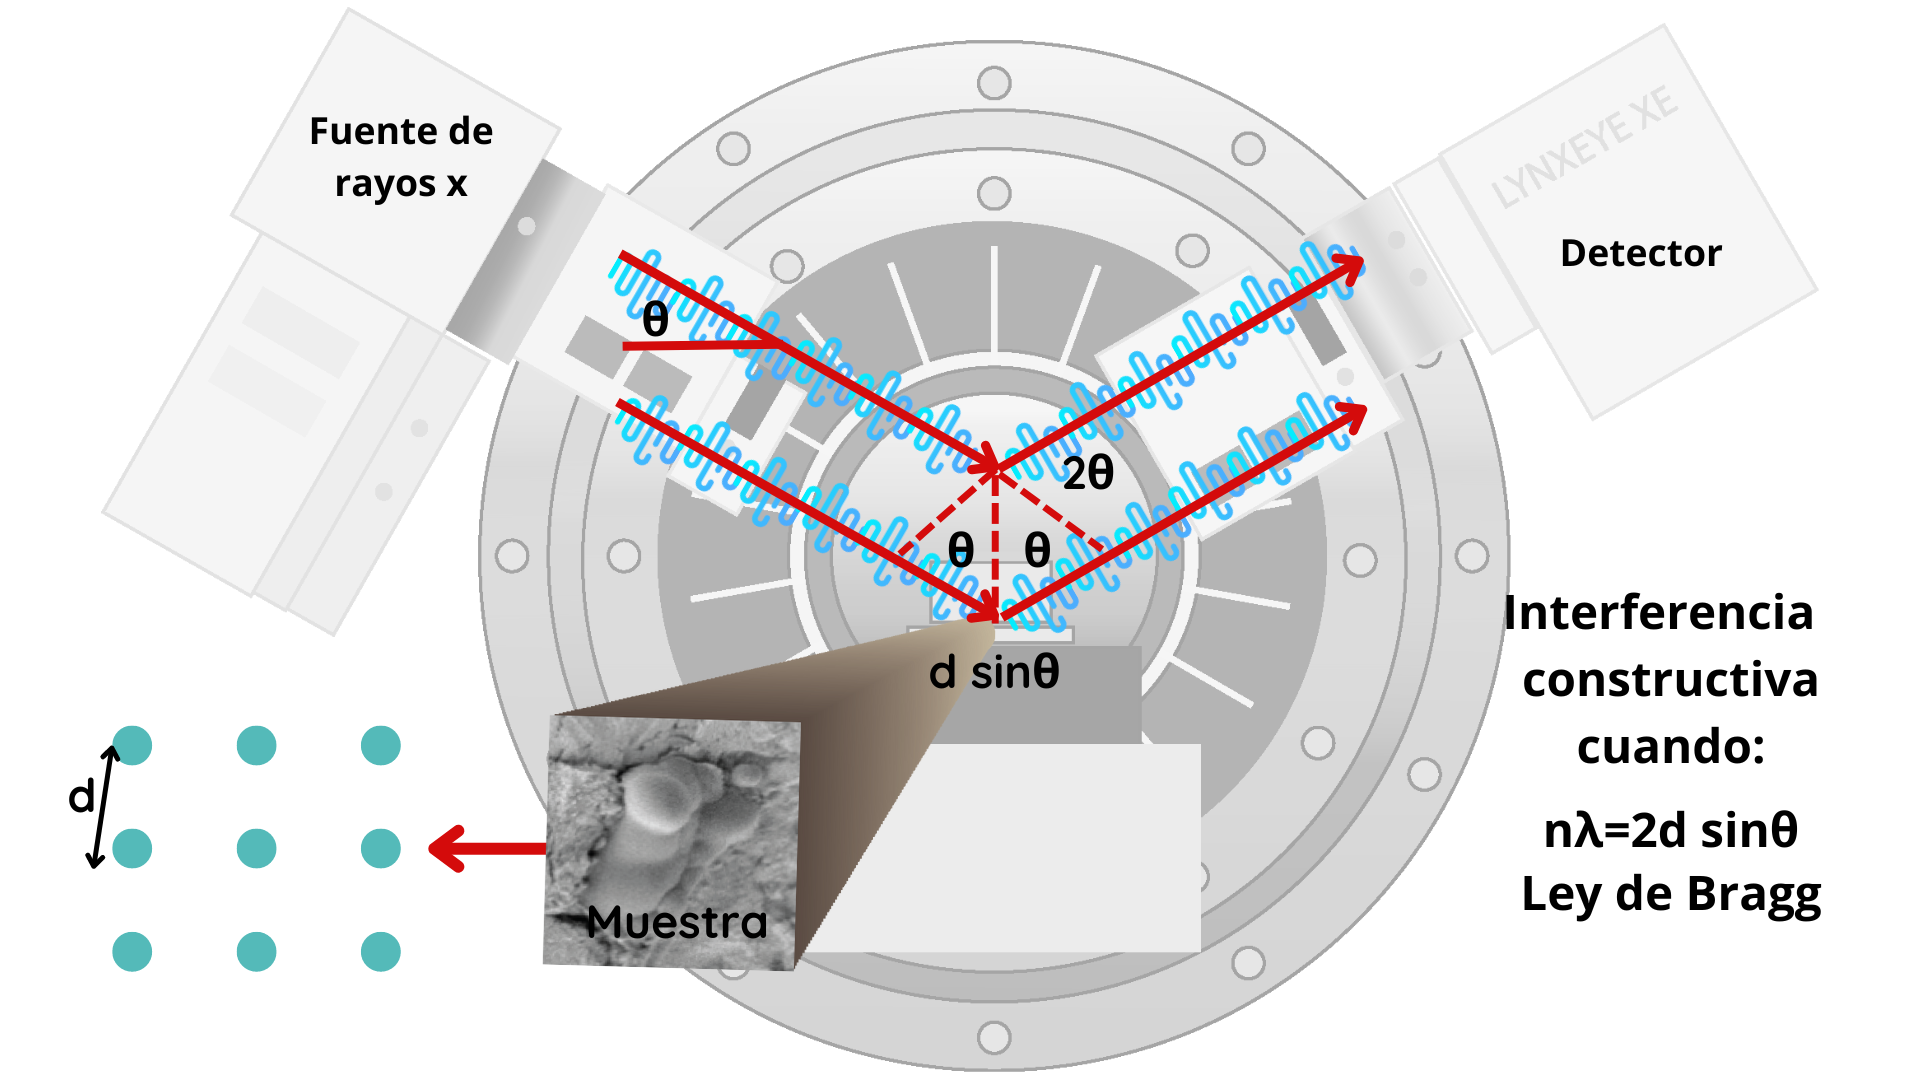
\includegraphics[width = 0.9\textwidth]{Imagenes/DRX.png}
     	  	\caption{Difractómetro de rayos X Bruker D8 Advance LinxEye. Fuente de rayos X: Tubo de descarga con ánodo de cobre (Kα1 = 0.1540 Å).
            Detector: unidimensional (LinxEye fast speed) con área activa de 14 mm x 16 mm y eficiencia 0.98.}\label{fig:DRX_1}  
    	   \end{center} 
        \end{figure}

        \subsubsection{Espectroscopia ultravioleta-visible (UV-VIS)}
        UV-Vis, abreviatura de Espectroscopia Ultravioleta-Visible, es una técnica utilizada para analizar la interacción de la luz ultravioleta (UV) y visible (Vis) con la materia. Es una técnica analítica ampliamente utilizada en diversos campos, incluyendo química, bioquímica, física y ciencia de materiales.\vspace{1em} % Espaciado adicional entre párrafos
        
        La espectroscopia UV-Vis mide la absorción de luz en las regiones UV y visible del espectro electromagnético. Cuando una muestra se expone a luz UV o visible, las moléculas en la muestra absorben fotones de energías específicas correspondientes a transiciones electrónicas dentro de las moléculas. La luz absorbida hace que los electrones en las moléculas se muevan desde su estado fundamental a un estado excitado.\vspace{1em} % Espaciado adicional entre párrafos
        
        El instrumento utilizado en la espectroscopia UV-Vis consta de una fuente de luz UV-Vis, un monocromador, un porta-muestras y un detector. La fuente de luz emite un espectro amplio de luz UV y visible, que luego se pasa a través del monocromador. El monocromador selecciona una longitud de onda específica o un rango de longitudes de onda para irradiar la muestra. Posteriormente, se detecta la luz transmitida o absorbida por la muestra mediante un detector, como en la Figura \ref{fig:UV_VIS_IMAGEN} \cite{IEEEreferencias:Ref1}.
        \begin{figure}[H]
    	   \begin{center}
     	  	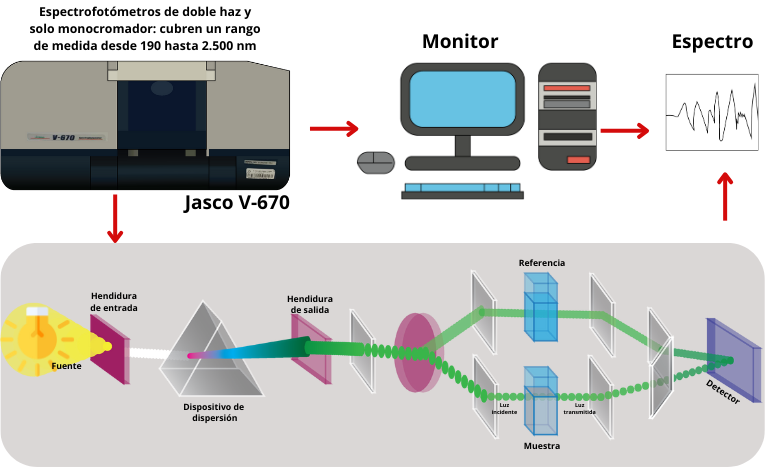
\includegraphics[width = 0.9\textwidth]{Imagenes/UV_VIS_IMAGEN.png}
     	  	\caption{UV-Vis, Proceso del espectroscopio UV-vis de la marca JASCO modelo V-670 que se encuentra en las instalaciones de la SEES, CINVESTAV.}{\label{fig:UV_VIS_IMAGEN} 
    	   \end{center} 
        \end{figure}
        
        El UV-vis, Jasco V-670, el espectrofotómetro de doble haz V-670 (Figura \ref{fig:UV_VIS_IMAGEN}) utiliza un diseño exclusivo de monocromador único que cubre un rango de longitud de onda de 190 a 2700 nm (opción de 3200 nm). El monocromador presenta rejillas duales (intercambiadas automáticamente): 1200 ranuras/mm para la región UV/VIS; 300 ranuras/mm para la región NIR. Se proporciona un detector PMT para la región UV/VIS y se emplea un detector PbS enfriado por Peltier para la región NIR. Tanto las rejillas como el detector se intercambian automáticamente dentro del rango seleccionable por el usuario de 800 a 900 nm.\vspace{1em} % Espaciado adicional entre párrafos

        Es importante destacar que la espectroscopia UV-Vis proporciona información sobre la absorción de luz por parte de las moléculas presentes en la muestra, lo que puede utilizarse para determinar la concentración de sustancias y determinar el bandgap del SnO$\displaystyle _{2}$ y ZnO a partir de la ecuación~\ref{eq:ecu4} de Tauc Ploc.\vspace{1em} % Espaciado adicional entre párrafos
 
        \begin{gather}
        ( \alpha hv)^{y } =A( hv-E_{g})
        \label{eq:ecu4}
        \end{gather}
        
        \begin{gather*}
        \begin{matrix}
        \alpha  & coeficiente\ de\ absorción\\
        h & constante\ de\ Planck\\
        v & la\ frecuencia\ del\ fotón\ incidente\\
        A & es\ una\ constante\ de\ proporcionalidad\\
         &  \begin{array}{l}
        ( esta\ determinada\ por\ el\ indie\ de\ refraccion,\ \\
        vale\ 1\ en\ materiales\ amorfos)
        \end{array}\\
        E_{g} & energía\ de\ banda\ prohibida\\
        y  & naturaleza\ de\ transicion\ electronica
        \end{matrix}\\
        \\
        \begin{array}{|c|}
        \hline
         \begin{array}{l}
        y =2\ es\ una\ transicion\ directa\ permitida\\
        y =1/2\ es\ una\ transicion\ indirecta\ permitida\\
        y =2/3\ es\ una\ transicion\ prohibida\ directa\\
        y =1/3\ es\ una\ transicion\ indirecta\ prohibida
        \end{array}\\
        \hline
        \end{array}\\
        \end{gather*}

        El término importante es el exponente y de la ecuación~\ref{eq:ecu4}, que denota la naturaleza de la transición electrónica. Típicamente, las transiciones permitidas dominan los procesos básicos de absorción, dando lugar a transiciones directas o indirectas.

        Para representar gráficamente $( \alpha hv)^{y}$ versus (hv) se debe probar el valor de transición permitido de y=2 o y=1/2 para comparar cuál nos proporciona el mejor ajuste de la recta tangente a la curva de los espectros en UV-vis, por lo tanto, identifica el tipo de transición correcto.\vspace{1em} % Espaciado adicional entre párrafos

        Para determinar la energía incidente se recurre a la ecuación~\ref{eq:Ehv}, la cual explica la relación entre la energía absorbida por la celda del UV-vis y la energía total que incide sobre ella.

        El coeficiente de absorción $\alpha$ de la Ecuación~\ref{eq:alpha}, determina la longitud que puede atravesar la luz a través de un material antes de ser absorbida. Este valor depende del tipo de luz y del material.

        
        \begin{gather}
        \label{eq:Ehv}
        E=hv:Energía\ incidente\\
         \notag\\
        E=hv=\frac{hc}{\lambda } =\frac{6.625\ \times 10^{-34}( Js) \times 2.998\times 10^{8}( m/s)}{\lambda ( m)}\\
        E=\frac{1.986\ \times 10^{-25} \times ( eVm)}{\lambda ( m) \times 1.602\times 10^{-19}} =\frac{1.240\times 10^{-6} \times ( eVm)}{\lambda ( m)}\\
        E=\frac{1240\times 10^{-9} \times ( eVm)}{\lambda ( m)} =\frac{1240\times \left( eV10^{-9} m\right)}{\lambda ( m)}\\
         \notag\\
        E=\frac{1240\times ( eVnm)}{\lambda ( nm)}\\
         \notag\\
        \begin{array}{|c|}
        \hline
        E=\frac{1240}{\lambda } eV\\
        \hline
        \end{array}\\
         \notag
        \end{gather}

        
        
        
        \begin{gather}
        \alpha :\ Coeficiente\ de\ absorción \notag\\\label{eq:alpha}
        I=I_{0} e^{-\alpha x}\\
        \frac{I}{I_{0}} =e^{-\alpha x} =e^{-\alpha l}\\
        \log\left(\frac{I}{I_{0}}\right) =\log\left( e^{-\alpha l}\right) =-\alpha l\log( e) =-\alpha l\log( 0.4343)\\
        \log\left(\frac{I}{I_{0}}\right) =A=\alpha l\log( 0.4343)\rightarrow \alpha =2.302\frac{A}{l}\\
        \begin{array}{|c|}
        \hline
        \alpha =2.302Acm^{-1}\\
        \hline
        \end{array}
        \end{gather}

        

       \subsubsection{Espectroscopia infrarroja por transformada de fourier (FTIR)}
        La Espectroscopia Infrarroja por Transformada de Fourier (FTIR), es una técnica de caracterización que se utiliza para estudiar la interacción de la radiación infrarroja con la materia. Permite analizar y caracterizar compuestos orgánicos e inorgánicos en muestras sólidas, líquidas o gaseosas, acciones realizadas por el equipo de la Figura \ref{fig:FTIR_EQUIPO}  \cite{IEEEreferencias:FTIR}.\vspace{1em} % Espaciado adicional entre párrafos

        La espectroscopia FTIR se basa en el principio de que las moléculas absorben la radiación infrarroja en determinadas frecuencias que corresponden a las vibraciones de los enlaces químicos presentes en la muestra. Al irradiar la muestra con luz infrarroja, se obtiene un espectro que muestra las intensidades de absorción en función de la frecuencia o el número de onda.
        \vspace{1em} % Espaciado adicional entre párrafos
        
        En la espectroscopia FTIR, se utiliza un interferómetro para generar un espectro interferométrico. Este espectro se somete a una transformada de Fourier para obtener el espectro infrarrojo final, que muestra las bandas de absorción correspondientes a las vibraciones moleculares.
        \vspace{1em} % Espaciado adicional entre párrafos
        
        El espectro FTIR proporciona información valiosa sobre la estructura química y la composición de la muestra. Cada banda de absorción en el espectro está asociada con un tipo específico de vibración molecular, como las vibraciones de estiramiento y flexión de los enlaces químicos. El análisis del espectro permite identificar los grupos funcionales presentes en la muestra, determinar la presencia de compuestos específicos y realizar análisis cuantitativos.\vspace{1em} % Espaciado adicional entre párrafos
        
        La espectroscopia FTIR se utiliza en una amplia gama de aplicaciones, incluyendo la química orgánica e inorgánica, la caracterización de materiales, el análisis de alimentos y medicamentos, el estudio de polímeros, el control de calidad y muchos otros campos de investigación y desarrollo \cite{IEEEreferencias:FTIR}.
        
        \begin{figure}[H]
            	   \begin{center}
             	  	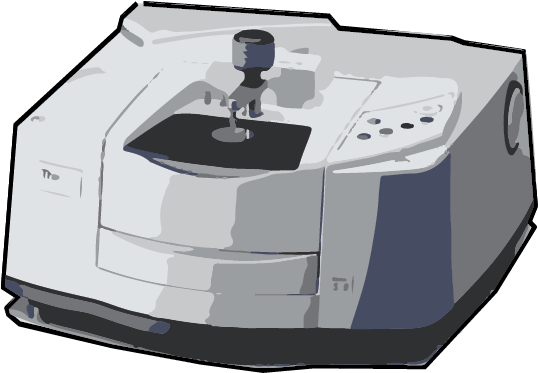
\includegraphics[width = 0.5
                 \textwidth]{Imagenes/FTIR_EQUIPO.png}
             	  	\caption{El espectro FTIR para las nanopartículas de GO co-dopadas con los iones Dióxido de estaño, fue realizada en un espectrómetro Nicolet-6700-FT-IR. Esta medición fue realizada en el Cinvestav.}
                 \label{fig:FTIR_EQUIPO} 
            	    \end{center} 
                \end{figure}
        \subsubsection{Espectroscopía Raman} 
            La Espectroscopia Raman es una técnica fotónica de alta resolución que proporciona en pocos segundos información química y estructural de materia orgánica e inorgánica, permitiendo así su estudio a detalle.\vspace{1em} % Espaciado adicional entre párrafos
                
            El análisis se realiza con la luz dispersada por un lente al incidir sobre él un haz de luz monocromático en vez de un haz de electrones. La luz es dispersada inelásticamente, experimentando ligeros cambios de frecuencia que son característicos del material analizado e independientes de la frecuencia de la luz incidente. Se trata de una técnica de análisis que no afecta la muestra, por lo que no es necesario protegerla con algún material.  \cite{IEEEreferencias:Ref15}\vspace{1em} % Espaciado adicional entre párrafos
                
            El equipo usado es un Jobin-Yvon T64000 de la Figura \ref{fig:raman_equipo}, con un láser verde de 514 cm$^{-1}$, un HORIBA-HR800 con un láser en una longitud de onda de 632.8 cm$^{-1}$, el cual se encuentra en las instalaciones del Cinvestav Zacatenco.Jobin Yvon T64000 Raman.\vspace{1em} % Espaciado adicional entre párrafos
        
        \begin{figure}[H]
            	   \begin{center}
             	  	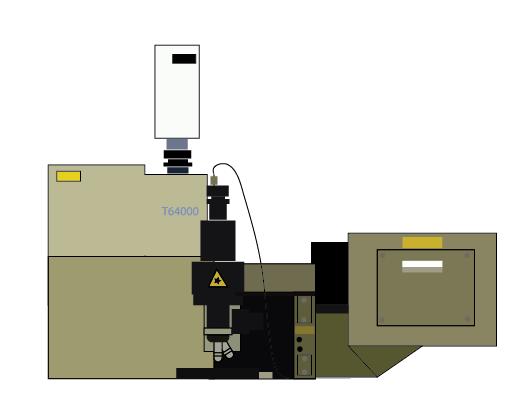
\includegraphics[width = 0.6\textwidth]{Imagenes/raman_equipo.png}
             	  	\captionof{figure}{\label{fig:raman_equipo}Raman, Jobin-Yvon T64000.} 
            	   \end{center} 
                \end{figure}
                
        \subsubsection{Espectroscopia XPS (X-ray Photoelectron Spectroscopy)}
        
        La espectroscopia XPS es una técnica de análisis de superficie que se utiliza para estudiar la composición química de la capa más externa de un material. Esta técnica se basa en la emisión de fotoelectrones por parte de los átomos en una muestra cuando son bombardeados con rayos X de alta energía. Para este tipo de técnica se utilizan equipos como el de la Figura \ref{fig:EquipoXPS}. \vspace{1em} % Espaciado adicional entre párrafos
        
        Los fotoelectrones emitidos son energéticamente característicos de los átomos a partir de los cuales provienen, lo que permite determinar la composición química y la estructura electrónica de la superficie de un material. La XPS se utiliza en una variedad de campos, como la química de superficies, la ciencia de los materiales y la nanotecnología, para investigar la composición y la química de las superficies de muestras sólidas \cite{IEEEreferencias:XPS}.
        
        \begin{figure}[H]
            	   \begin{center}
             	  	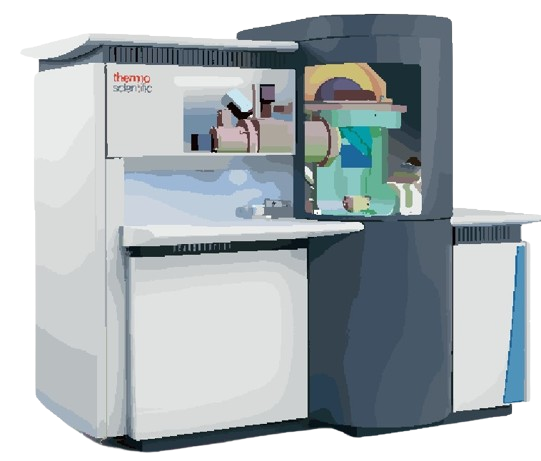
\includegraphics[width = 0.5\textwidth]{Imagenes/EquipoXPS.png}
             	  	\captionof{figure}{\label{fig:EquipoXPS}Espectrómetro de fotoelectrones emitidos por rayos X K-Alpha XPS.} 
            	   \end{center} 
                \end{figure}
        
         
        \subsubsection{Microscopia Electrónica de Barrido (SEM)}
            SEM (Scanning Electron Microscopy) es una técnica de caracterización de nanomateriales, funciona a partir de las señales resultantes de la interacción entre la materia y un haz de electrones, como se ilustra en la Figura \ref{fig:SEM_EQUIPO}. Es posible la detección, procesamiento y visualización de imágenes de muestras que serían imposibles de observar para el ojo humano.  La información recabada de los microscopios electrónicos de barrido sirve para identificar la composición, topografía y estructura de la muestra analizada. Este tipo de herramienta permite el estudio de objetos sólidos, orgánicos e inorgánicos (flores, insectos, polen) \cite{IEEEreferencias:Ref13}.
                El equipo que se utilizó fue el microscopio Zeiss-AURIGA en las instalaciones de LANE, CINVESTAV Zacatenco.
        \begin{figure}[H]
            	   \begin{center}
             	  	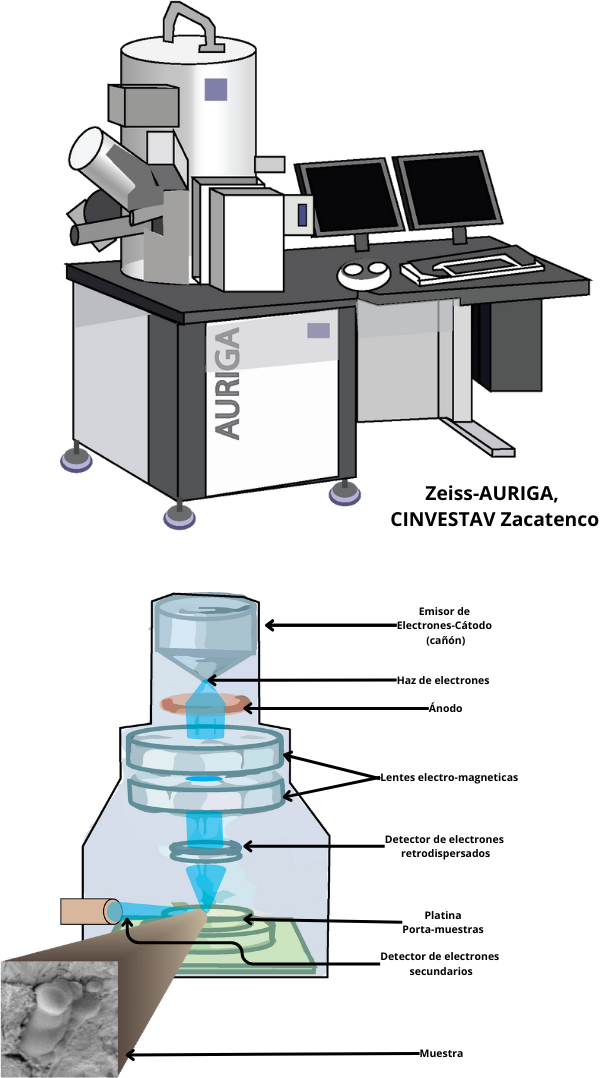
\includegraphics[width = 0.7\textwidth]{Imagenes/SEM_EQUIPO.png}
             	  	\captionof{figure}{\label{fig:SEM_EQUIPO}Microscopia Electrónica de Barrido (SEM) con el equipo Zeiss-AURIGA, del cinvestav Zacatenco y como funciona internamente.} 
            	   \end{center} 
                \end{figure}
        

\newpage
\section{Desarrollo Experimental}
En el desarrollo experimental del presente trabajo de investigación se eligió replicar la síntesis de Hummer para la obtención de GO y para la obtención de los semiconductores de SnO$\displaystyle _{2}$ y ZnO se optó por usar la síntesis hidrotermal replicando metodologías experimentales \cite{IEEEreferencias:Ref36}.\vspace{1em} % Espaciado adicional entre párrafos

La forma experimental consiste en cambiar una de las condiciones de síntesis para los semiconductores, en el caso de SnO$\displaystyle _{2}$ se experimentó con el mejor tiempo de tamaño cristalino y variando el tiempo de reacción de 10, 20, 30 y 40 h. Para después hacer variaciones en la concentración de precursor para el decorado del GO de 0.1,0.2, 0.4 y 1 M.\vspace{1em} % Espaciado adicional entre párrafos

Para el ZnO sé vario el pH de 9 a 11 a las mismas condiciones de tiempo y temperatura para la síntesis hidrotermal. Para después hacer variaciones en la concentración de precursor para el decorado del GO de 0.1,0.2 y 0.4 M. Tomando en cuenta las características de los materiales empleados en las Tablas \ref{CuadroGO}, \ref{CuadroSnO2} y \ref{CuadroZnO}.\vspace{1em} % Espaciado adicional entre párrafos
\begin{table}[h]
\centering
\caption{Características de los reactivos para la síntesis de GO.}
\begin{tabular}{|c|c|c|c|}
\hline
\textbf{Reactivo} & \textbf{Nombre} & \textbf{Función} & \textbf{Características} \\ 
\hline
Grafito 
& Forma cristalina del carbono 
& Precursor 
& Estructura en capas \\ 
\hline
NaNO$_3$ 
& Nitrato de sodio 
& Oxidante 
& Facilita la oxidación durante la síntesis \\ 
\hline
H$_2$SO$_4$ 
& Ácido sulfúrico 
& Exfolia 
& Medio altamente ácido \\ 
\hline
KMnO$_4$ 
& Permanganato de potasio 
& Oxidante 
& Genera grupos funcionales \\ 
\hline
\end{tabular}
\label{CuadroGO}
\end{table}

\begin{table}[h]
\centering
\caption{Características de los reactivos para la síntesis de SnO$_2$.}
\begin{tabular}{|c|c|c|c|}
\hline
\textbf{Reactivo} & \textbf{Nombre} & \textbf{Función} & \textbf{Características} \\ 
\hline
SnCl$_{4} \ \smblkcircle \ 5$H$_{2}$O 
& \begin{tabular}[c]{@{}l@{}}
Cloruro de estaño \\ 
tetravalente \\ 
pentahidratado
\end{tabular} 
& Precursor 
& Alta pureza y soluble en agua \\ 
\hline
NaOH 
& Hidróxido de sodio 
& Reductor 
& Base fuerte \\ 
\hline
\end{tabular}
\label{CuadroSnO2}
\end{table}


\begin{table}[h]
\centering
\caption{Características de los reactivos para la síntesis de ZnO.}
\begin{tabular}{|c|c|c|c|}
\hline
\textbf{Reactivo} & \textbf{Nombre} & \textbf{Función} & \textbf{Características} \\ 
\hline
Zn(CH$_{3}$COO)$_{2} \ \smblkcircle \ 2$H$_{2}$O 
& \begin{tabular}[c]{@{}l@{}}
Acetato de zinc \\ 
dihidratado
\end{tabular} 
& Precursor 
& \begin{tabular}[c]{@{}l@{}}
Soluble en \\ 
agua y etanol
\end{tabular} \\ 
\hline
NaOH 
& Hidróxido de sodio 
& Reductor 
& Base fuerte \\ 
\hline
\end{tabular}
\label{CuadroZnO}
\end{table}


    \subsection{Síntesis de GO por el método de Hummer}
    El procedimiento para la síntesis del material se llevó a cabo siguiendo los pasos que se ilustran en la Figura~\ref{fig:Hummer1} y \ref{fig:Hummer2}. A continuación, se detalla cada etapa \cite{IEEEreferencias:ZnOGO_Fotocatalisis_1,IEEEreferencias:ZnOGO_Fotocatalisis_2, IEEEreferencias:ZnOGO_Fotocatalisis_3}.
    
    \begin{enumerate}
    \item \textbf{Preparación de la solución inicial:}En un matraz Erlenmeyer de 500 ml, se añadió grafito (Grafito (C): 2.0065 g), nitrato de sodio (NaNO$_3$: 1.0039 g) y ácido sulfúrico concentrado (H$_2$SO$_4$: 46 ml de ácido concentrado) previamente enfriado a 0 °C. 

    \item\textbf{Oxidación del grafito:}Esta mezcla se mantuvo en un baño de hielo, con agitación vigorosa y lentamente se añadió permanganato de potasio (KMnO$_4$: 6.0765 g) teniendo cuidado que la temperatura no superara los 20 °C. Después de 5 minutos, la mezcla fue retirada del baño de hielo y agitada durante 1 h a 35±3 °C. La reacción simplificada es:
     \[
    \text{C} + \text{KMnO}_4 + \text{H}_2\text{SO}_4 + \text{NaNO}_3 \rightarrow \text{Grafito Oxidado (óxido de grafeno)} + \text{Otros productos}
    \]
    \begin{align}
    \text{Masa de grafito inicial} &= 2.0065 \, \text{g} \\
    \text{Masa molar del grafito (C)} &= 12 \, \text{g/mol} \\
    \text{Moles de grafito} &= \frac{2.0065 \, \text{g}}{12 \, \text{g/mol}} = 0.1672 \, \text{moles}
    \end{align}
    
    \item\textbf{Enfriamiento:} Se añadió lentamente agua desionizada (92 ml). Se mantuvo la agitación durante 15 minutos y a continuación se agregaron 140 ml de agua a \textasciitilde 60 °C, así como 5 ml de una solución de peróxido de hidrógeno al 30\%. El volumen total de la solución después de añadir los 92 ml de agua a las 46 ml de H$_2$SO$_4$ es de 0.143 L.
    
    \item\textbf{Agitación: } 
    Los materiales obtenidos en medio acuoso se sometieron a 2 h de ultrasonido.

    \item\textbf{Lavado:}En este punto se observaron dos productos, uno amarillo-café y otro negro. Los cuales fueron recuperados y lavados con agua tibia hasta alcanzar un pH cercano a 7.

    \item\textbf{Precipitación:}Los productos se centrifugaron varias veces a 4000 rpm durante 30 minutos.

    \item\textbf{Secado:}Finalmente, los materiales obtenidos en medio acuoso se sometieron a 2 h de ultrasonido para combinarlo con el SnO$\displaystyle _{2}$ y el ZnO.

    \item\textbf{Calcinación:}La muestra de GO se colocó en una mufla para ser calcinado a 190 °C por 20 h para mandarlo a analizar.
    
    \end{enumerate}
    
    Usamos la cantidad de moles de grafito convertidos y el volumen total de la solución para calcular la molaridad:
    \begin{align}
    \text{Molaridad (M)} &= \frac{\text{moles de óxido de grafeno}}{\text{volumen de la solución en litros}} \\
    &= \frac{0.1672 \, \text{moles}}{0.143 \, \text{L}} \\
    &= 1.129\, \text{M pero lo consideraremos como 1M}
    \end{align}


        \begin{figure}[H]
        	\begin{center}
         		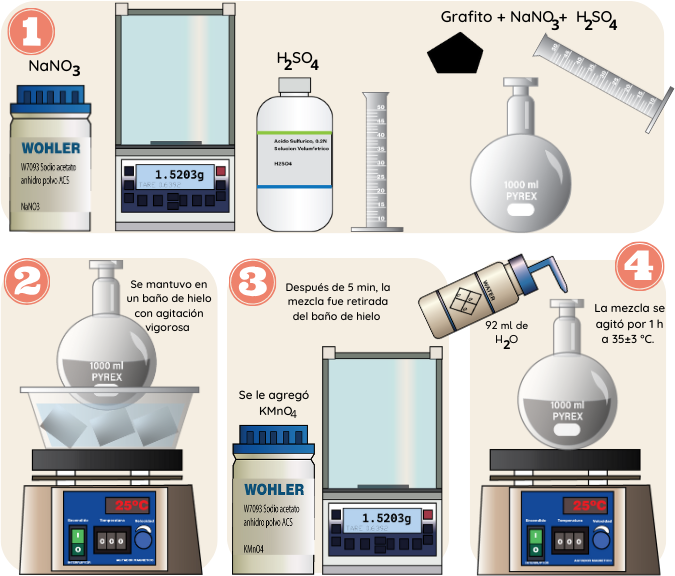
\includegraphics[width = 0.9\textwidth]{Imagenes/GO_1.png}
         		\captionof{figure}{\label{fig:Hummer1}Síntesis  de Hummer para obtener GO, explicación del paso 1 al paso 4.} 
        	\end{center} 
        \end{figure}
         \begin{figure}[H]
        	\begin{center}
         		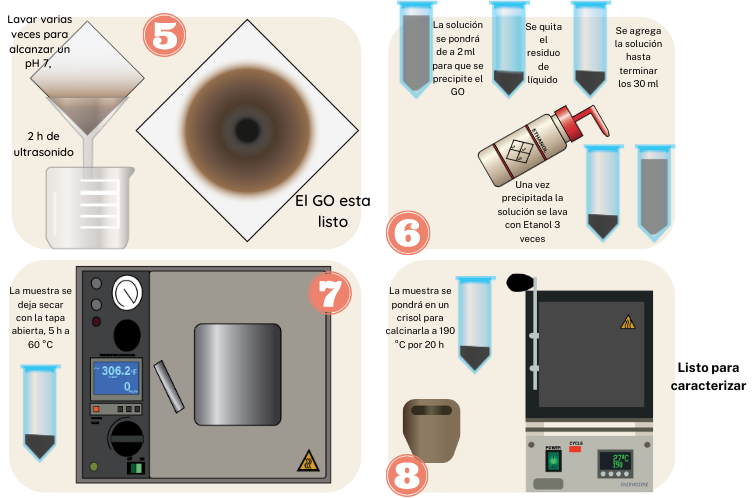
\includegraphics[width = 0.9\textwidth]{Imagenes/GO_2.png}
         		\captionof{figure}{\label{fig:Hummer2}Síntesis de Hummer para obtener GO, explicación del paso 5 al paso 8.} 
        	\end{center} 
        \end{figure}

        
        \subsection{Síntesis de SnO$\displaystyle _{2}$ }
        El procedimiento para la síntesis del material se llevó a cabo siguiendo los pasos que se ilustran en la Figura \ref{fig:SnO2_1} y \ref{fig:SnO2_2}. A continuación, se detalla cada etapa: 


        \begin{enumerate}
        \item\textbf{Preparación de la solución inicial:}Para calcular la cantidad necesaria de $\displaystyle SnCl_{4} \smblkcircle 5H_{2} O$ y NaOH para obtener \ 0.1 M de $\displaystyle SnO_{2}$ en una síntesis solvotérmica, primero conoceremos las estequiometrías de las reacciones químicas involucradas.
        
        La reacción de síntesis de $\displaystyle SnO_{2}$ \ a partir de $\displaystyle SnCl_{4} \smblkcircle 5H_{2} O$ y NaOH es la siguiente:
        
        \begin{equation}
        \ {\displaystyle SnCl_{4} \smblkcircle 5H_{2} O} \ +\ 2\ NaOH\ \rightarrow \ {\displaystyle SnO_{2}} +\ 2\ NaCl\ +\ 7\ {\displaystyle H_{2} O}
        \end{equation}

        Entonces, para obtener 0.1 M \ de SnO$\displaystyle _{2}$, se necesita:
        
        \begin{gather}
        n=\frac{0.1M}{0.08\ L} =0.008\ moles\\
        {\displaystyle PM_{SnO_{2}} =} 150.71\ g/mol\\
        \ \ \ \ \ \ \ \  \notag\\
        \ \ \ \ \ \ \ \ {\displaystyle m_{SnO_{2}} =150.71g/mol*0.008=\textcolor[rgb]{0.29,0.56,0.89}{1.2057g\ \ de\ SnO_{2}}}\\
         \notag
        \end{gather}
        
        
        \item\textbf{Precursor:} Dado que la relación estequiométrica es 1:1, se necesita la misma cantidad de moles de $\displaystyle SnCl_{4} \smblkcircle 5H_{2} O$ que de $\displaystyle SnO_{2}$ :
        
        Ahora, se calcula la cantidad de $\displaystyle SnCl_{4} \smblkcircle 5H_{2} O$ en gramos:
       
        \begin{gather}
        \ \ \ {\displaystyle n_{SnCl_{4} \smblkcircle 5H_{2} O} =} \ {\displaystyle 0.008\ moles\ de\ SnCl_{4} \smblkcircle 5H_{2} O}\\
        \ \ \ \ \ \ \ \  \notag\\
        \ \ \ \ \ \ \ \ {\displaystyle PM_{SnCl4\smblkcircle 5H2O} =} 350.57\ g/mol\\
        \ \ \ \ \ \ \ \  \notag\\
        \ \ \ \ \ \ \ \ {\displaystyle m_{SnCl_{4} \smblkcircle 5H_{2} O} =} 0.008\ moles\ *\ 350.57\ g/mol\ \\
        \ {\displaystyle m_{SnCl_{4} \smblkcircle 5H_{2} O}} =\ 2.805\ gramos\ de\ {\displaystyle SnCl_{4} \smblkcircle 5H_{2} O}
        \end{gather}

        
        \item \textbf{Reductor:}Para la cantidad de NaOH necesaria, la relación estequiométrica es 2 moles de NaOH por 1 mol de $\displaystyle SnCl_{4} \smblkcircle 5H_{2} O$. Por lo tanto, necesitas el doble de moles de NaOH que de $\displaystyle SnCl_{4} \smblkcircle 5H_{2} O$:
        
        \begin{gather}
        {\displaystyle n_{NaOH} =} 2\ *\ 0.008\ moles\ \approx \ 0.016\ moles\ de\ NaOH.\ \ \ \ \ \ \ \\
        \ \ \ \ \ \ \ \ {\displaystyle PM_{NaOH} =40\ g/mol} \ \\
        \ \ \ \ \ \ \ \ {\displaystyle m_{NaOH}} =0.016\ moles\ *\ 40\ g/mol\ \approx \textcolor[rgb]{0.29,0.56,0.89}{0.64\ gramos\ de\ NaOH}
        \end{gather}
        
        Por lo tanto, para obtener 1.2057 gramos de SnO$\displaystyle _{2}$ en la síntesis solvotérmica, necesitas aproximadamente 2.805 gramos de $\displaystyle SnCl_{4} \smblkcircle 5H_{2} O$ y 0.64 gramos de NaOH en una mezcla de 40 ml de etanol y 40 ml de agua. 
        \item\textbf{Agitación:} Una vez hecha la solución, se debe de agitar en la parrilla magnética a una baja velocidad durante 24 h para colocar la solución en una autoclave para el tratamiento térmico.
        
        \item\textbf{Tratamiento térmico:} De acuerdo a la autoclave que se utilice, en este caso se utilizó una autoclave de 50 ml, pero siempre se debe de llenar al 70\% de su capacidad máxima, se van a seguir los pasos anteriores pero con las condiciones de tiempo y temperatura de la Tabla \ref{tab:tabla_muestras}, que nos marca la metodología de \cite{IEEEreferencias:Ref36}.
        
        \begin{table}[h]
        \caption{Condiciones de las muestras de SnO$_{2}$}
        \centering
        \begin{tabular}{|c|c|c|}
        \hline
        Muestra & Grados Celsius & Tiempo en horas\\
        \hline
        A.SnO$_{2}$ & 190 & 48\\
        \hline
        B.SnO$_{2}$ & 190 & 24\\
        \hline
        C.SnO$_{2}$ & 160 & 20\\
        \hline
        D.SnO$_{2}$ & 100 & 20\\
        \hline
        \end{tabular}
        \label{tab:tabla_muestras}
        \end{table}

        \item\textbf{Precipitación:} Después de las pruebas en el horno, lo siguiente es lavar las muestras tres veces con etanol y poner en la centrifugadora a 5000 rpm para precipitar nuestro nanomaterial.
        \item\textbf{Secado:}Una vez lavados, se dejan secar con la tapa abierta en el horno a 65\ºC, ya que el plástico se puede derretir a 80\ºC.
        \item\textbf{Calcinación:} Una vez secas, las muestras se dejan en crisoles dentro de una mufla a 190\ºC por 20 h, para quitarles a los nanocristales impurezas o residuos de etanol y agua que se evaporan a 100\ºC.
         \end{enumerate}

        \begin{figure}[H]
        	\begin{center}
         		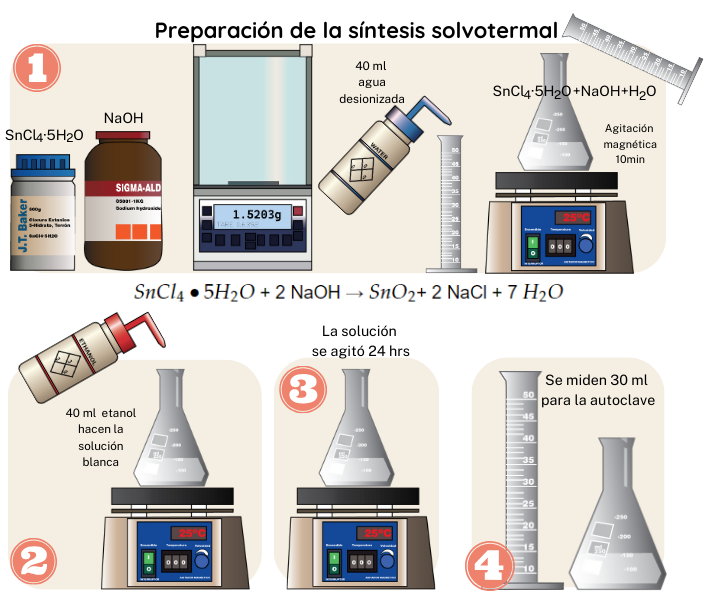
\includegraphics[width = 0.8\textwidth]{Imagenes/SnO2_sintesis_1.png}
         		\captionof{figure}{\label{fig:SnO2_1}Descripción visual de la síntesis del óxido de estaño por el método solvotermal .} 
        	\end{center} 
        \end{figure}
        \begin{figure}[H]
        	\begin{center}
         		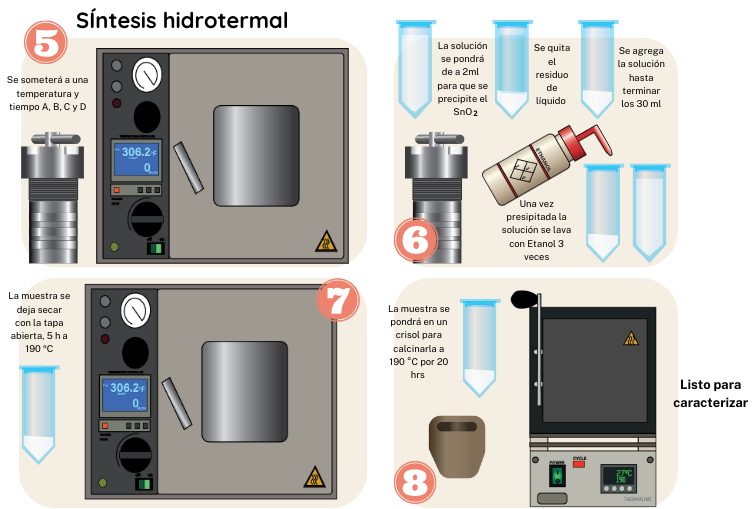
\includegraphics[width = 0.8\textwidth]{Imagenes/SnO2_sintesis_2.png}
         		\captionof{figure}{\label{fig:SnO2_2}Descripción visual de la síntesis del oxido de estaño por el metodo hidrotermal.} 
        	\end{center} 
        \end{figure}
    
        \subsubsection{Preparación de los sistemas de SnO$\displaystyle _{2}$@GO}
        El procedimiento para el decorado del SnO$\displaystyle _{2}$ y GO se llevó a cabo siguiendo los pasos que se ilustran en la Figura \ref{fig:SnO2_GO_AZ_R6G}. A continuación, se detalla cada etapa:
        
         \begin{enumerate}
            \item \textbf{Preparación de la solución inicial}:Se aplicó la síntesis hidrotermal en un solo recipiente para preparar nanopartículas de SnO$\displaystyle_{2}$-rGO. En la solución inicial se agregó 2,804 g de SnCl$_{4} \cdot 5$H$_{2}$O y 0.64 g de NaOH a 20 mL de agua desionizada como muestran los valores de la Tabla\ref{tab:tabla_naoh_sncl4}.
            
            \item \textbf{Adición del GO a la solución de SnO$\displaystyle _{2}$:} Como medio de reacción se dispersaron 20 mL de etanol y 40 mL de GO en agua.
            
            \item \textbf{Preparar autoclave:}Luego, la mezcla se agitó durante 24 horas para obtener una solución homogénea. Se transfirió de la solución solo 30 mL a un autoclave de acero inoxidable con capacidad para 50 mL.
            
            \item \textbf{Tratamiento térmico:} Las condiciones 
            de temperatura y tiempo se eligieron al experimentar con el SnO$_{2}$, que nos dio el tamaño de cristal más pequeño para 160 ◦C durante 30 h. Luego, el producto se centrifugó, se lavó 3 veces con etanol y agua deshidratada, y se secó a 70 ◦C durante 18 h para obtener nanopartículas de SnO2-rGO. Se estudió el cambio en la concentración del medio de reacción de agua desionizada y etanol con un cambio en la molaridad de 0,1, 0,125, 0,15 y 0,175 M como se observa en la Tabla \ref{tab:tabla_muestras_sno2_GO}.
            
            \item \textbf{Quitar impurezas:}Las muestras se colocaron en un crisol cada una para someterlas por medio de una mufla a calcinación durante un tiempo de 20 h y una temperatura de 190\ºC. 
            
            \item \textbf{Lámpara UV-C:}Las muestras calcinadas se muelen con un mortero para pesar 0.1 g para hacer pruebas en oscuro y con lámpara UV-C con cada catalizador decorado con GO, para el GO, para el SnO$\displaystyle _{2}$ individual y para los colorantes individuales. Estas pruebas se analizarán cada 15 min hasta completar un tiempo de 180 min. 
            \item \textbf{Pruebas de absorbancia:} Una vez que se realizaron las pruebas en el UV-vis, se calculara el porcentaje de degradación, para comparar los catalizadores puros de los decorados y así se determinara si la hipótesis es correcta.
            
         \end{enumerate}

    \begin{table}[h]
    \caption{Datos de NaOH y SnCl$_{4} \cdot 5$H$_{2}$O.}
    \centering
    \begin{tabular}{|c|c|c|c|c|}
    \hline
     & PM (g/mol) & m & V & Soluto\\
    \hline
    NaOH & 40 & 0.08 & 1/2 & Etanol\\
    \hline
    SnCl$_{4} \cdot 5$H$_{2}$O & 350.57 & 0.35 & 1/2 & Agua desionizada\\
    \hline
    \end{tabular}
    \label{tab:tabla_naoh_sncl4}
    \end{table}
    
    \begin{table}[h]
    \caption{Datos de las muestras de SnO$_{2}$.}
    \centering
    \begin{tabular}{|c|c|c|c|c|c|}
    \hline
    Muestra & M (mol) & V (ml) & m (NaOH g) & m (SnCl$_{4} \cdot 5$H$_{2}$O g) & m (SnO$_{2}$ g) & PM (SnO$_{2}$ g/mol) & n\\
    \hline
    10SnO$_{2}$ & 0.1 & 10 & 0.08 & 0.35 & 0.1507\\
    \hline
    5SnO$_{2}$ & 0.2 & 5 & 0.08 & 0.35 & 0.1507\\
    \hline
    2.5SnO$_{2}$ & 0.4 & 2.5 & 0.08 & 0.35 & 0.1507\\
    \hline
    1SnO$_{2}$ & 1 & 1 & 0.08 & 0.35 & 0.1507\\
    \hline
    \end{tabular}
    \label{tab:tabla_muestras_sno2_GO}
    \end{table}
    
             \begin{figure}[H]
            	\begin{center}
             		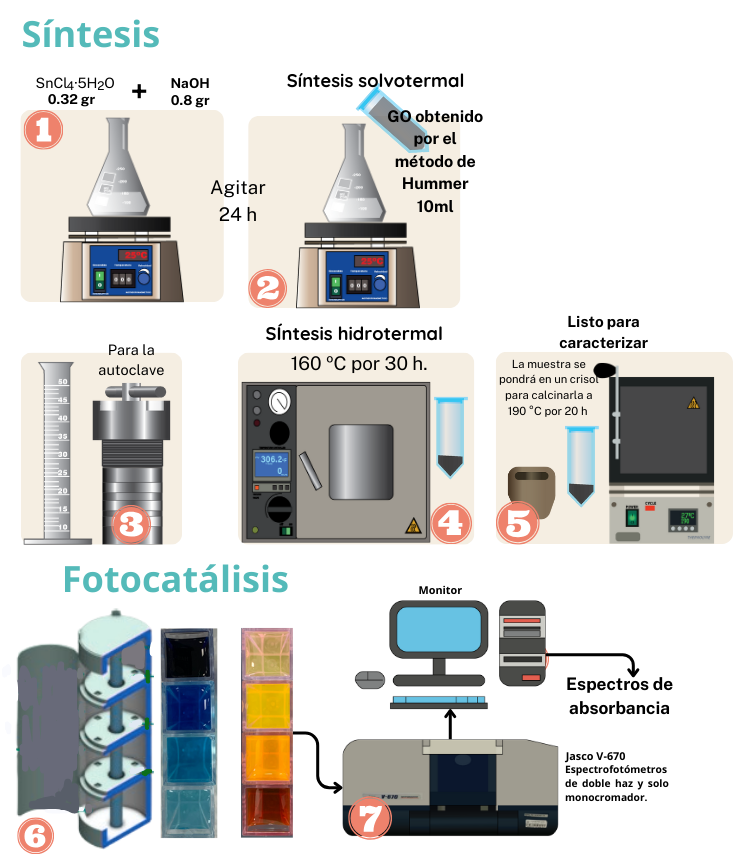
\includegraphics[width = 0.75\textwidth]{Imagenes/CARTEL.png}
             		\captionof{figure}{\label{fig:SnO2_GO_AZ_R6G}Descripción visual del decorado de dióxido de estaño y GO por el método hidrotermal.} 
            	\end{center} 
            \end{figure}        
    
      \subsection{Síntesis de ZnO }
    El procedimiento para la síntesis del ZnO se llevó a cabo siguiendo los pasos que se ilustran en la Figura \ref{fig:SÍntesis ZnO_1} y \ref{fig:SÍntesis ZnO_2}. A continuación, se detalla cada etapa:



    \begin{enumerate}
        \item\textbf{Preparación de la solución inicial:}Para calcular la cantidad necesaria de $\displaystyle Zn( CH_{3} COO)_{2} \smblkcircle 2H_{2} O$ y NaOH para obtener una molaridad de 0.1 M de $\displaystyle ZnO$ en una síntesis solvotérmica, primero es importante conocer las estequiometrías de las reacciones químicas involucradas. La reacción de síntesis de ZnO para un precursor de $\displaystyle Zn(CH_{3} COO)_{2} \smblkcircle 2H_{2} O$ y NaOH es la siguiente:        
        \begin{equation}
        Zn( CH_{3} COO)_{2} \smblkcircle 2H_{2} O\ +\ 2\ NaOH\ \rightarrow \ ZnO\ +\ 2\ CH_{3} COONa\ +\ 3\ H_{2} O
        \label{eq:ecuZnO}
        \end{equation}

        Para determinar una aproximación del producto con una molaridad del 0.1 M \ de ZnO, es necesario:

        \begin{gather}
        \ n=\frac{0.1M}{0.08\ L} =0.008\ moles\\
        \ {\displaystyle PM_{ZnO} =} 81.38\ g/mol\ \ \ \ \\
        \ \ \ \ \ \ \ \ {\displaystyle m_{ZnO} =81.38\ g/mol*0.008=\textcolor[rgb]{0.29,0.56,0.89}{0.65104\ g\ \ de\ ZnO}}
        \end{gather}
        
        
        Dado que la relación estequiométrica es 1:1, se necesita la misma cantidad de moles de $\displaystyle Zn( CH_{3} COO)_{2} \smblkcircle 2H_{2} O$ que de ZnO :
    
    
        
        Ahora, la cantidad de $\displaystyle Zn( CH_{3} COO)_{2} \smblkcircle 2H_{2} O$ en gramos:
    

            
        \begin{gather}
        {\displaystyle n_{Zn(CH_{3} COO)_{2} \smblkcircle 2H_{2} O} =} \ {\displaystyle 0.008\ moles\ de\ Zn(CH_{3} COO)_{2} \smblkcircle 2H_{2} O} \ \ \ \\
        {\displaystyle PM_{Zn(CH_{3} COO)_{2} \smblkcircle 2H_{2} O} =} 219.51\ g/mol\ \\
        {\displaystyle m_{n(CH_{3} COO)_{2} \smblkcircle 2H_{2} O} =} 0.008\ moles\ *\ 219.51\ g/mol\ \\
        {\displaystyle m_{n(CH_{3} COO)_{2} \smblkcircle 2H_{2} O} =}\textcolor[rgb]{0.29,0.56,0.89}{1.75608\ g\ de{\displaystyle \ Zn(CH_{3} COO)_{2} \smblkcircle 2H_{2} O}}
        \end{gather}
          \item\textbf{Agitación magnética:} El precursor se va a agregar a 40 ml de agua desionizada y 40 ml de etanol para su agitación en una parrilla magnética durante 15 min.
          
         \item\textbf{Variar el pH:}Para la variación del pH se añadirá cuidadosamente gota a gota NaOH como se observa en la Tabla \ref{tab:PHZNO}, ya que puede hacer un salto abrupto. 
                 \begin{table}[h!]
            \centering
            \caption{Condiciones de síntesis para las muestras en función del pH.}
            \begin{tabular}{|c|c|c|c|}
                \hline
                Muestra & Tiempo (h) & Temperatura (°C) & \(\mu\)L \\
                \hline
                13pH & 4.5 & 120 & 460 \\
                12pH & 4.5 & 120 & 420 \\
                11pH & 4.5 & 120 & 360 \\
                10pH & 4.5 & 120 & 240 \\
                9pH  & 4.5 & 120 & 200 \\
                \hline
            \end{tabular}
            \label{tab:PHZNO}
        \end{table}

         
         Pero para preparación general de NaOH la relación estequiométrica es 2 moles de NaOH por 1 mol de $\displaystyle Zn( CH_{3} COO)_{2} \smblkcircle 2H_{2} O$. Por lo tanto, se necesita de:  
            \begin{gather}
            {\displaystyle n_{NaOH} =} 2\ *\ 0.008\ moles\ \approx \ 0.016\ moles\ de\ NaOH.\\
            \ \ \ \ \ \ \ \ \ \ \ \ {\displaystyle PM_{NaOH} =40\ g/mol} \ \\
            \ \ \ \ \ \ \ \ \ \ \ \ {\displaystyle m_{NaOH}} =0.016\ moles\ *\ 40\ g/mol\ \approx \textcolor[rgb]{0.29,0.56,0.89}{0.64\ gramos\ de\ NaOH}
            \end{gather}
        \item\textbf{Reactivos:}Por lo tanto, para obtener 0.65104 g de ZnO en la síntesis solvotérmica, es necesario aproximadamente 1.75608 g de $\displaystyle Zn( CH_{3} COO)_{2} \smblkcircle 2H_{2} O$ y 0.64 gramos de NaOH en una mezcla de 40 ml de etanol y 40 ml de agua.
        
        \begin{figure}[H]
        	\begin{center}
         		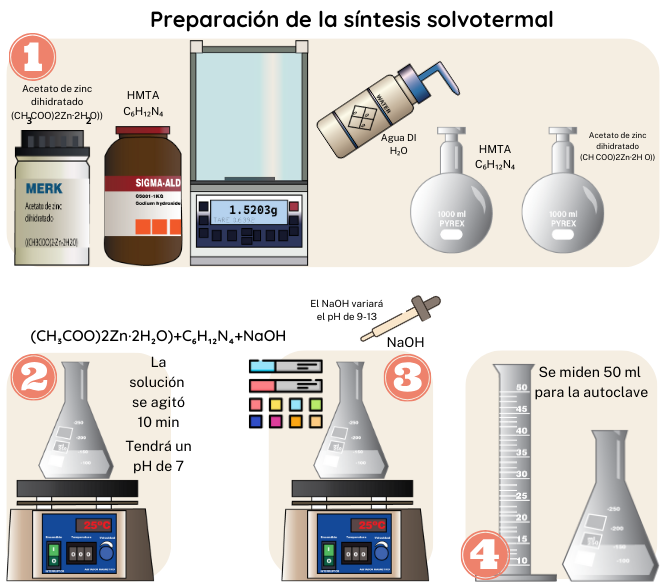
\includegraphics[width = 0.65\textwidth]{Imagenes/SÍntesis ZnO_1.png}
         		\captionof{figure}{\label{fig:SÍntesis ZnO_1}Descripción visual de los pasos 1 al 4 de la preparación por la síntesis hidrotermal del ZnO.} 
        	\end{center} 
        \end{figure}

        \item\textbf{Síntesis hidrotermal:} De acuerdo a la autoclave que se utilice, en este caso se utilizó una autoclave de 50 ml, pero siempre se debe de llenar al 70\% de su capacidad máxima, las condiciones de tiempo y temperatura son de 4.5 h por 120 \ºC.
        
        \item\textbf{Lavado:}  Después de las pruebas en el horno, lo siguiente es lavar las muestras tres veces con etanol y poner en la centrifugadora a 5000 rpm para precipitar nuestro nanomaterial.
        
        \item\textbf{Secado:}Una vez lavados, se dejan secar con la tapa abierta en el horno a 65\ºC, ya que el plástico se puede derretir a 80\ºC. 
        
         \end{enumerate}
        
        \begin{figure}[H]
        	\begin{center}
         		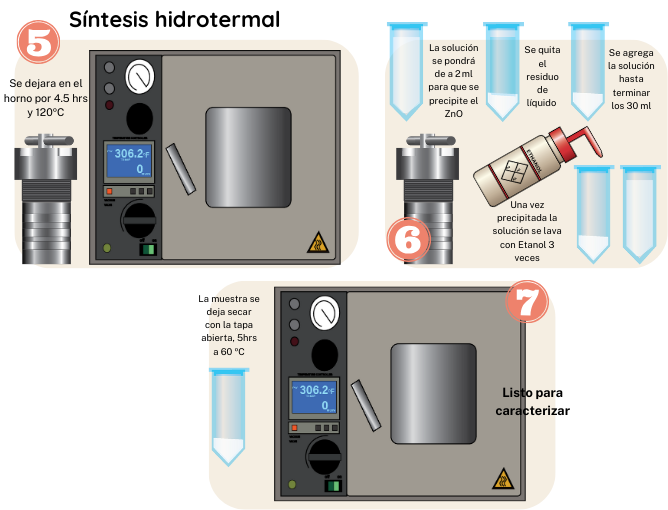
\includegraphics[width = 0.8\textwidth]{Imagenes/SÍntesis ZnO_2.png}
         		\captionof{figure}{\label{fig:SÍntesis ZnO_2}Descripción visual de los pasos 5 al 7 de la preparación por la síntesis hidrotermal del ZnO.} 
        	\end{center} 
        \end{figure}
\subsubsection{Preparación de los sistemas de ZnO@GO}
    El procedimiento para el decorado del ZnO y GO se llevó a cabo siguiendo los pasos que se ilustran en la Figura \ref{fig:ZnO_GO_Sintesis}. A continuación, se detalla cada etapa:
        \begin{enumerate}
            \item \textbf{Preparación de la solución inicial}:Para llevar a cabo la síntesis hidrotermal de ZnO y óxido de grafeno (GO), primero se debe preparar una solución con las sustancias necesarias. Para obtener una molaridad final de 0.1 M de ZnO, se disuelven 1.756 gramos de Zn (CH₃COO)₂·2H₂O en agua desionizada, como se observa en la Tabla \ref{tabla_naoh_znch3coo}.
            
            \item \textbf{Adición del GO a la solución de SnO$\displaystyle _{2}$:} Como medio de reacción se dispersaron 20 mL de etanol y 40 mL de GO en agua.
            
            \item \textbf{Preparar autoclave:}Luego, la mezcla se agitó durante 10 min para obtener una solución homogénea. Se transfirió de la solución solo 30 mL a un autoclave de acero inoxidable con capacidad para 50 mL.
            
            \item \textbf{Tratamiento térmico:} Las condiciones 
            de temperatura, ph y tiempo se eligieron al experimentar con el ZnO puro, que nos dio el tamaño de cristal más pequeño para 120 ◦C durante 4.5 h a un ph de 11. Luego, el producto se centrifugó, se lavó 3 veces con etanol y agua deshidratada, y se secó a 70 ◦C durante 18 h para obtener nanopartículas de ZnO-rGO. Se estudió el cambio en en la masa del precursor para variar la molaridad de 0,1, 0,2 y 0,4 M como se observa en la Tabla \ref{tab:ZnOGO}.
             
            
            \item \textbf{Lámpara UV-C:}Las muestras se muelen con un mortero para pesar 0.1 g para hacer pruebas en oscuro y con lámpara UV-C con cada catalizador decorado con GO, para el GO, para el ZnO individual y para los colorantes individuales de R6G y AM. Estas pruebas se analizarán cada 15 min hasta completar un tiempo de 180 min. 
            \item \textbf{Pruebas de absorbancia:} Una vez que se realizaron las pruebas en el UV-vis, se calculara el porcentaje de degradación, para comparar los catalizadores puros de los decorados y así se determinara si la hipótesis es correcta.
            
         \end{enumerate}
\begin{table}[h]
\caption{Datos de NaOH y Zn(CH$_{3}$COO)$_{2} \cdot 2$H$_{2}$O.}
\centering
\begin{tabular}{|c|c|c|c|c|}
\hline
 & PM (g/mol) & m (g) & V (ml) & Soluto\\
\hline
NaOH & 40 & 0.08 & 25 & Agua desionizada\\
\hline
Zn(CH$_{3}$COO)$_{2} \cdot 2$H$_{2}$O & 219.51 & 0.65 & 25 & Agua desionizada\\
\hline
\end{tabular}
\label{tabla_naoh_znch3coo}
\end{table}


\begin{table}[ht]
    \centering
      \caption{Muestras de ZnO con sus respectivos valores de mol, volumen (ml) y masa (g)}
    \begin{tabular}{|c|c|c|c|}
        \hline
        Muestra & M (mol) & V (ml) & m (g) \\
        \hline
        ZnO & 0.0 & 50 & 0.0 \\
        \hline
        2.5\%ZnO & 0.1 & 50 & 0.274 \\
        \hline
        5\%ZnO & 0.2 & 50 & 0.548 \\
        \hline
        10\%ZnO & 0.4 & 50 & 1.097 \\
        \hline
        \end{tabular}
    \label{tab:ZnOGO}
\end{table}


\begin{figure}[H]
        	\begin{center}
         		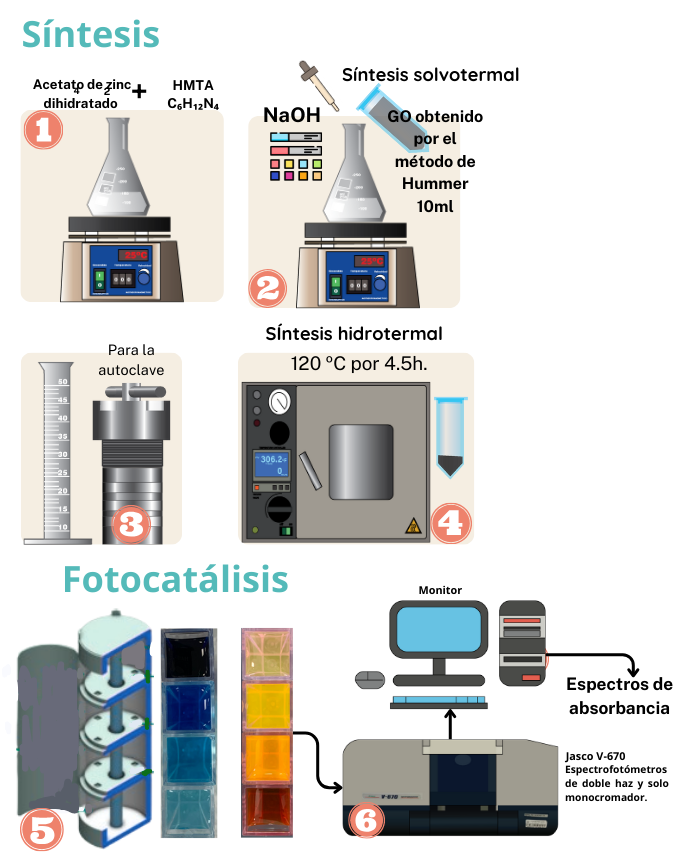
\includegraphics[width = 1\textwidth]{Imagenes/ZnO_GO_Sintesis.png}
         		\captionof{figure}{\label{fig:ZnO_GO_Sintesis}Descripción visual de los pasos 1 al 6 de la preparación por la síntesis hidrotermal del decorado del ZnO con GO.} 
        	\end{center} 
        \end{figure}

\newpage
\section{Discusión y análisis de resultados}
 La caracterización de estos nanomateriales es fundamental para entender y optimizar sus propiedades estructurales, ópticas y electrónicas, las cuales son determinantes para su eficiencia fotocatalítica.\vspace{1em} % Espaciado adicional entre párrafos

A través de técnicas como espectroscopia Raman, difracción de rayos X (XRD), espectroscopia XPS, microscopía electrónica (SEM/TEM), espectroscopia infrarroja por transformada de fourier (FTIR) y análisis UV-Vis, podemos describir aspectos clave como el tamaño de partícula, la morfología, la cristalinidad y la capacidad de absorción de luz.\vspace{1em} % Espaciado adicional entre párrafos 

Estos parámetros están intrínsecamente relacionados con la actividad fotocatalítica, ya que afectan directamente la generación de pares electrón-hueco y la formación de radicales hidroxilo, esenciales para la degradación de contaminantes.\vspace{1em} % Espaciado adicional entre párrafos

En este contexto, las pruebas fotocatalíticas nos permiten evaluar el rendimiento de estos nanomateriales bajo condiciones específicas de iluminación, midiendo su capacidad para descomponer compuestos modelo como colorantes (rodamina 6G o azul de metileno). Este enfoque experimental es crucial para correlacionar las propiedades estructurales y electrónicas de los nanomateriales con su desempeño en aplicaciones prácticas de descontaminación ambiental.\vspace{1em} % Espaciado adicional entre párrafos

Mediante esta caracterización integral, buscamos identificar las condiciones y modificaciones que maximicen la eficiencia fotocatalítica, contribuyendo así al desarrollo de tecnologías sostenibles para la protección del medio ambiente.

Las condiciones de 

\subsection{Discusión y análisis de resultados del GO}
Una vez sintetizado y secado, el GO se llevará a pruebas de caracterización de DRX, UV-vis, FTIR, Raman y SEM para identificar sus caracterizaciones antes de ser decorado por el SnO$\displaystyle _{2}$ y el ZnO. También se evaluará como se comporta ante pruebas fotocataliticas ante colorantes como el azul de metileno y rodamina 6G.
\subsubsection{DRX}
Los espectros de difracción de rayos X (DRX) del óxido de grafeno (GO) de la Figura \ref{fig:DRX_GO}, muestran dos picos de difracción característicos que confirman la estructura del material de acuerdo \cite{IEEEreferencias:GO_3}. En el espectro DRX de GO, se observan dos picos principales:
\vspace{1em} % Espaciado adicional entre párrafos

Un pico agudo a aproximadamente 2θ = 10°-11°, correspondiente al plano (001) del GO. Este pico indica la presencia de grupos oxigenados en la estructura del grafeno, lo que resulta en un aumento en la distancia interplanar debido a la inserción de oxígenos y otros grupos funcionales entre las capas de grafeno \cite{IEEEreferencias:GO_2}.
Un segundo pico más amplio y menos intenso alrededor de 2θ = 42°, que puede atribuirse al plano (100) del GO. Este pico sugiere la presencia de una pequeña cantidad de grafeno reducido o de regiones no completamente oxidadas dentro de la estructura del GO \cite{IEEEreferencias:GO_3}.
\vspace{1em} % Espaciado adicional entre párrafos

\begin{figure}[H]
    	   \begin{center}
     	  	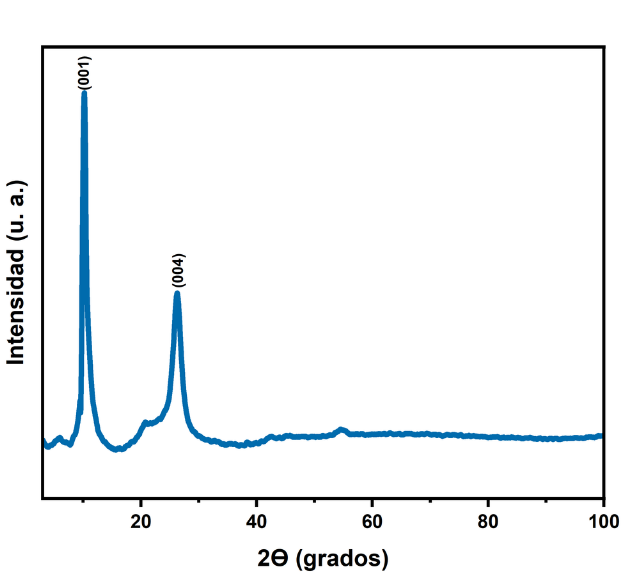
\includegraphics[width = 0.8\textwidth]{Imagenes/GO_1_2.png}
     	  	\captionof{figure}{\label{fig:DRX_GO}Patrón de difracción de rayos x del óxido de grafeno (GO). } 
    	   \end{center} 
        \end{figure}
\subsubsection{UV-vis}
Para el estudio en UV- vis del GO, SnO$\displaystyle _{2}$ y ZnO se utilizó el espectroscopio UV-vis de la marca JASCO modelo V-670 que se encuentra en las instalaciones de la SEES, CINVESTAV de la Figura \ref{fig:UV_VIS_IMAGEN}.
El espectro UV-Vis del óxido de grafeno (GO) de la Figura \ref{fig:UV_GO} proporciona información clave sobre sus propiedades electrónicas y ópticas. En el caso del GO, el espectro presenta características distintivas que reflejan la presencia de grupos oxigenados y la estructura alterada del grafeno.\vspace{1em} % Espaciado adicional entre párrafos
Se visualiza un hombro de absorción a aproximadamente 300 nm, el cual es asociado con las transiciones n→π* de los grupos funcionales oxigenados, tales como los carbonilos y epóxidos, que están presentes en la superficie del GO. La presencia de este hombro confirma la incorporación de oxígeno en la estructura del grafeno.\vspace{1em} % Espaciado adicional entre párrafos

Además de estos picos de absorción, el análisis del espectro UV-Vis permite la estimación del band gap del GO. Utilizando el método de Tauc de la ecuación~\ref{eq:ecu4}, con una transición directa permitida de 2, el band gap del GO se ha calculado con una pendiente que cruza aproximadamente en un calor de 2.408 eV. Este valor indica una brecha energética significativa, mayor que la del grafeno puro, lo cual es consistente con la introducción de defectos y grupos oxigenados que interrumpen la estructura conjugada del grafeno.\vspace{1em} % Espaciado adicional entre párrafos

\begin{figure}[H]
    	   \begin{center}
     	  	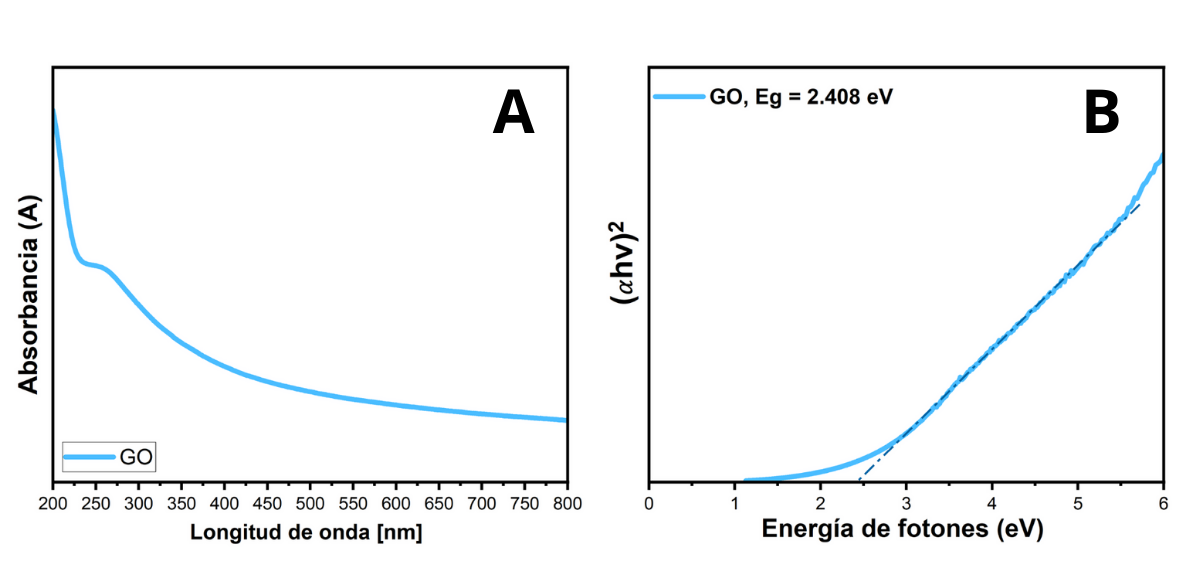
\includegraphics[width = 1\textwidth]{Imagenes/GO_BandGab_2.png}
     	  	\captionof{figure}{\label{fig:UV_GO} A, espectro de absorbancia en UV-vis del óxido de grafeno. B, band gab calculado por el método de Tauc Plot. } 
    	   \end{center} 
        \end{figure}
        
\subsubsection{FTIR}
El espectro de Infrarrojo por Transformada de Fourier (FTIR) del óxido de grafeno (GO) proporciona información detallada sobre los grupos funcionales presentes en la superficie del material. Las principales bandas de absorción observadas en el espectro FTIR del GO y sus respectivas asignaciones son las siguientes:\vspace{1em} % Espaciado adicional entre párrafos


En la Tabla \ref{tab:modos_vibracionales} se describen los grupos químicos que se localizan de acuerdo al número de onda del espectro de la Figura \ref{fig:FTIR_GO}, estas bandas se atribuyen a la presencia de grupos hidroxilo y agua adsorbida en la superficie del GO y que no están presentes en el grafeno puro \cite{IEEEreferencias:GO_2,IEEEreferencias:GO_4,IEEEreferencias:GO_8}.\vspace{1em} % Espaciado adicional entre párrafos


El espectro FTIR del GO muestra claramente la presencia de diversos grupos funcionales oxigenados, lo que confirma la modificación de la estructura del grafeno a través de la oxidación. Estos grupos funcionales, como los hidroxilos, epóxidos, carbonilos y carboxilos, no solo alteran la estructura electrónica del grafeno, sino que también son importantes en la fotocatálisis para oxidar cromóforos \cite{IEEEreferencias:GO_GOr}.
\begin{figure}[H]
    	   \begin{center}
     	  	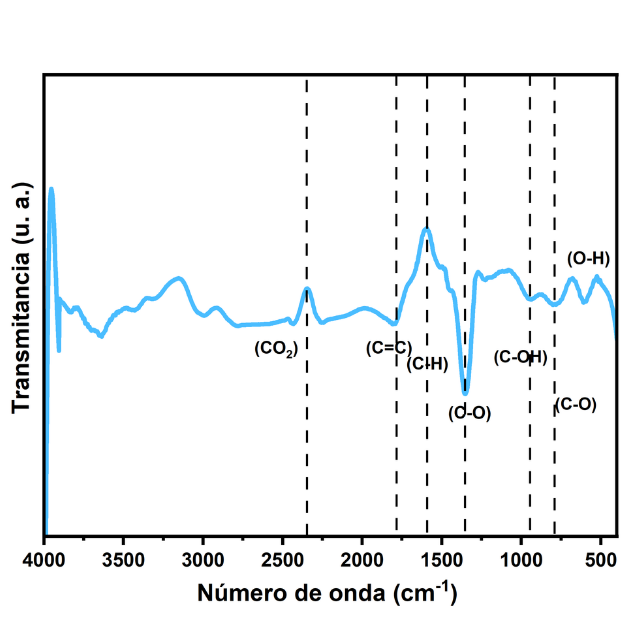
\includegraphics[width = 0.8\textwidth]{Imagenes/GO_FTIR.png}
     	  	\captionof{figure}{\label{fig:FTIR_GO}Espectro en FTIR del GO. } 
    	   \end{center} 
        \end{figure}


        \begin{table}[h!]
\centering
\caption{Modos vibracionales y números de onda característicos para diferentes grupos químicos.}
\begin{tabular}{|c|c|c|}
\hline
\textbf{Grupo químico} & \textbf{Modo vibracional} & \textbf{Número de onda} ($\text{cm}^{-1}$) \\ \hline
O-H                    & Estiramiento              & 3400                                        \\ \hline
C=O                    & Estiramiento              & 1729                                        \\ \hline
C=C                    & Estiramiento              & 1620                                        \\ \hline
C-O-C                  & Estiramiento              & 1220                                        \\ \hline
C-O-H                  & Estiramiento              & 1050                                        \\ \hline

\end{tabular}
\label{tab:modos_vibracionales}
\end{table}
\subsubsection{RAMAN}
El espectro RAMAN del óxido de grafeno (GO) de la Figura \ref{fig:RAMAN_GO}, proporciona información valiosa sobre la estructura y la calidad del material, especialmente después de la oxidación del grafeno. Las principales características observadas en el espectro RAMAN del GO incluyen:\vspace{1em} % Espaciado adicional entre párrafos

Banda D (~1350 cm⁻¹): Esta banda está asociada con la vibración de defectos estructurales y desorden en la red de carbono. En el GO, la presencia de grupos funcionales oxigenados y defectos introducidos durante la oxidación contribuye significativamente a esta banda \cite{IEEEreferencias:GO_GOr}.\vspace{1em} % Espaciado adicional entre párrafos

Banda G (~1580 cm⁻¹): La banda G es característica del modo de vibración E₂g del grafeno, que corresponde a las vibraciones de estiramiento de los enlaces C-C sp² en una red de grafeno ordenada. Aunque el GO está oxidado y presenta cierto desorden, la banda G aún es prominente, indicando la persistencia de regiones de grafeno no oxidado \cite{IEEEreferencias:GORAMAN}.\vspace{1em} % Espaciado adicional entre párrafos

El espectro RAMAN del GO de la Figura \ref{fig:RAMAN_GO} refleja la combinación de estructuras de grafeno oxidado y regiones de grafeno no oxidado que coexisten en el material. La relación entre las intensidades de las bandas D y G, proporcionan información sobre el grado de oxidación, el desorden estructural y la preservación de la estructura del grafeno en el GO.
\begin{figure}[H]
    	   \begin{center}
     	  	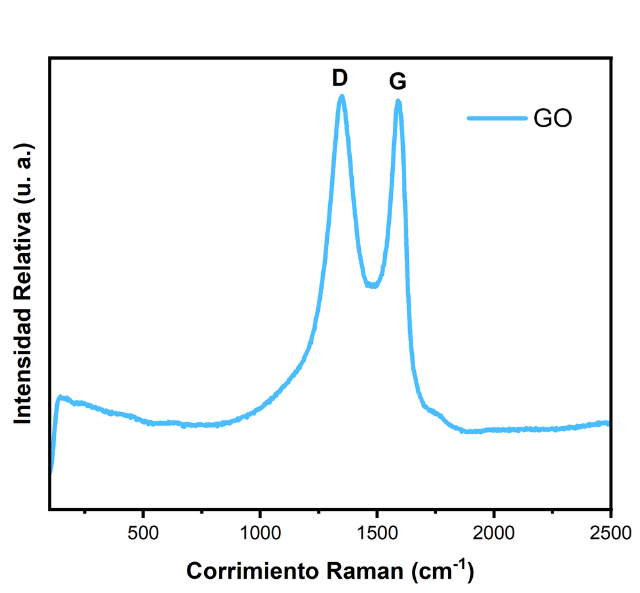
\includegraphics[width = 0.8\textwidth]{Imagenes/GO_RAMAN.png}
     	  	\captionof{figure}{\label{fig:RAMAN_GO} Espectro RAMAN del óxido de grafeno para la banda D y G. } 
    	   \end{center} 
        \end{figure}
        
\subsubsection{SEM}
El análisis por Microscopía Electrónica de Barrido (SEM) de la Figura \ref{fig:GO_SEM_1} del óxido de grafeno (GO) proporciona una visualización detallada de la morfología superficial y la estructura del material a 1 µm a 2.0 kV. Durante el análisis SEM del GO, se observan dos características importantes:\vspace{1em} % Espaciado adicional entre párrafos

\textbf{Estructura Laminar:} El GO muestra una estructura laminar, caracterizada por capas delgadas y planas dispuestas de manera ordenada. Estas capas son visibles en las imágenes SEM como estructuras planas y extendidas, indicativas de la estructura de hoja única del GO \cite{IEEEreferencias:GO_GOr}.\vspace{1em} % Espaciado adicional entre párrafos

\textbf{Superficie Rugosa:} Debido a la oxidación y los grupos funcionales, la superficie del GO presenta rugosidades y protuberancias irregulares. Estas características son evidentes en las imágenes SEM de la Figura \ref{fig:GO_SEM_1}, donde se observan superficies con textura, con detalles estructurales finos y regiones de mayor y menor densidad de defectos \cite{IEEEreferencias:GORAMAN}.\vspace{1em} % Espaciado adicional entre párrafos

\begin{figure}[H]
    	   \begin{center}
     	  	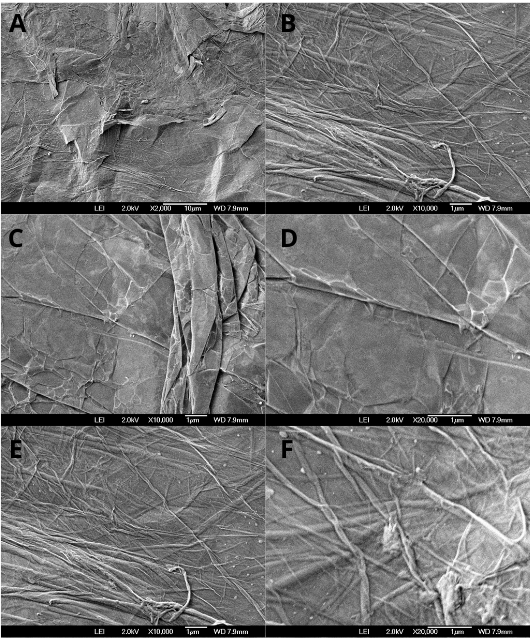
\includegraphics[width = 1\textwidth]{Imagenes/GO_SEM_1.png}
     	  	\captionof{figure}{\label{fig:GO_SEM_1}Microscopia electrónica de barrido del óxido de grafeno.  } 
    	   \end{center} 
        \end{figure}
\subsection{Discusión y análisis de resultados del SnO$\displaystyle _{2}$}     
Una vez sintetizados y secados los catalizadores de SnO$\displaystyle _{2}$ se analizarán por DRX y con base en los resultados se elegirá el catalizador con las mejores condiciones de tiempo y temperatura para luego variar el tiempo. Una vez obtenido, los catalizadores se caracterizarán por DRX, UV-vis, FTIR, RAMAN y SEM, para identificar sus características fotocatalíticas como menor banda ancha, el de tamaño cristalino más pequeño, el de mayor presencia de grupos funcionales oxigenados y el de una morfología con nanoesferas aglomeradas. \vspace{1em} % Espaciado adicional entre párrafo
\subsubsection{DRX}    
Las muestras se caracterizaron con la técnica de difracción de rayos x con el equipo del CICQS Difractómetro de rayos X Bruker D8 Advance LinxEye, con condiciones de 2θ de 20° a 80°, 30 kV, 25 mA, 0.03°/paso, 0.3 s/paso. Fuente de rayos X: Tubo de descarga con ánodo de cobre (Kα1 = 0.1540 Å). Detector: unidimensional (LinxEye fast speed) con área activa de 14 mm x 16 mm y eficiencia del 0.98 de la Figura \ref{fig:DRX_1}.\vspace{1em} % Espaciado adicional entre párrafo

Para el estudio de un semiconductor que funcione como fotocatalizador capaz de acelerar la reacción  se replicó la investigación \cite{IEEEreferencias:Ref36} de dióxido de estaño por síntesis hidrotermal, donde se utilizó como precursor él ($\displaystyle SnCl_{4} \cdotp 5H_{2} O$)  y como reductor NaOH lo que nos dio un pH ácido de 3. Para el uso de la autoclave se siguió la metodología para las 4 muestras etiquetadas como A, B, C y D, la primera a 190 °C y 48 h, la segunda a 190 °C a 48 h, la tercera a 160 °C a 20 h y la última a 100 °C a 20 h, cada una con secado de 24 h y sin calcinar.\vspace{1em} % Espaciado adicional entre párrafo

El  primer espectro de la Figura \ref{fig:SnO2_SinCalcinado_ABCD.png} que se visualiza es amorfo, ya que se formó por la síntesis solvotermal, en donde no hay presencia de condiciones térmicas. Las siguientes cuatro muestras se sometieron a las condiciones de síntesis hidrotermal. Es posible distinguir picos de difracción que indexan con la carta cristalográfica JCPDS 00-001-0667, que corresponde al dióxido de estaño con una estructura cristalina de rutilo.\vspace{1em} % Espaciado adicional entre párrafos

Con ayuda del software Origin 2023, se graficaron los espectros de la Figura \ref{fig:SnO2_SinCalcinado_ABCD.png} y se calculó con la ecuación \ref{eq:ecu3} de Scherrer el tamaño promedio de los cristalitos con los tres picos característicos que se encuentran en los índices de Miller (110), (200) y (220), donde la prueba C tiene un tamaño cristalino de 7,3646 nm que lo convierten en la prueba más pequeña y podemos distinguir en la Tabla \ref{tab:drx1}, que el tamaño del FWHM (Full Width at Half Maximum) o la anchura a media altura es inversamente proporcional al tamaño promedio del cristalito.\vspace{1em} % Espaciado adicional entre párrafos


\begin{figure}[H]
    	   \begin{center}
     	  	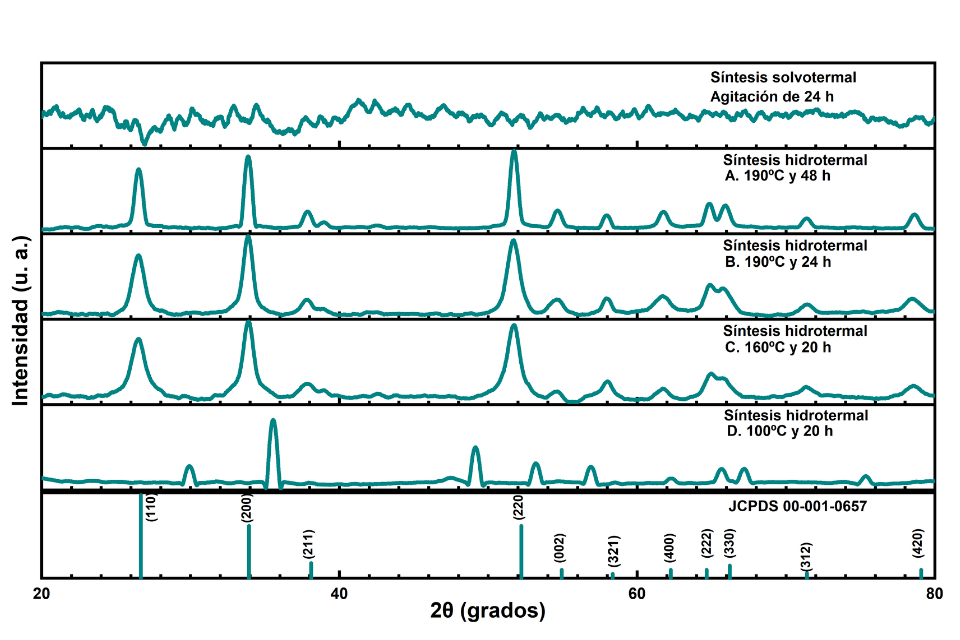
\includegraphics[width = 1\textwidth]{Imagenes/SnO2_SinCalcinado_ABCD.png}
     	  	\captionof{figure}{\label{fig:SnO2_SinCalcinado_ABCD.png}Patrón de difracción de rayos x del dióxido de estaño sin calcinar. } 
    	   \end{center} 
        \end{figure}




\begin{table}[h!]
 \caption{Tamaño cristalino promedio siguiendo la metodología sin calcinar de Talebiann y Jafarinezhad \cite{IEEEreferencias:Ref36}.}
  \centering
  \begin{tabular}{|c|c|c|c|c|c|}
    \hline
    Muestra & Picos & Posición (x) & FWHM & Tamaño (nm) & L (nm)\\
    \hline
    & (110) & 26.52059 & 0.48232 & 16.80 & \\
    A & (200) & 33.87299 & 0.32529 & 25.40 & \textcolor[rgb]{0.16,0.77,0.82}{21.109}\\
    & (220) & 37.85314 & 0.39518 & 21.12 & \\
    \hline
    & (110) & 26.48485 & 1.07081 & 7.55 & \\
    B & (200) & 33.86481 & 0.6704 & 12.29 & \textcolor[rgb]{0.16,0.77,0.82}{6.868}\\
    & (220) & 43.82059 & 11.03726 & 0.77 & \\
    \hline
    & (110) & 26.49445 & 1.76546 & 4.58 & \\
    C & (200) & 33.87809 & 0.963 & 8.55 & \textcolor[rgb]{0.16,0.77,0.82}{7.252}\\
    & (220) & 37.83798 & 0.96376 & 8.63 & \\
    \hline
  \end{tabular}
  \label{tab:drx1}
\end{table}

Con respecto a la prueba D de la metodología, se puede decir que sus picos de difracción no coinciden con la carta cristalográfica a diferencia de las demás pruebas a presión y temperatura, se tiene entonces fases mezcladas de SnO y SnO$\displaystyle _{2}$. Por lo que el patrón original no está corrido, no al menos por causa del equipo, está corrido por la presencia mayoritaria de una de esas dos fases. El patrón original considera cualitativamente y cuantitativamente ambas fases y su corrimiento (“aparente”) respecto de los de SnO$\displaystyle _{2}$ es consecuencia de las dos fases en conjunto y que predomine una más que la otra.\vspace{1em} % Espaciado adicional entre párrafos

Por lo que se decidió calcinar en la mufla las siguientes muestras a 24 h a 190 °C cada una para obtener la estructura cristalina deseada, como en la Figura \ref{fig:SnO2_Calcinado_ABCD}, donde se aprecia, que coinciden los picos de difracción y el tamaño promedio de los 3 picos cristalinos disminuye, por lo que el calcinar mejora nuestra muestra cristalina.\vspace{1em} % Espaciado adicional entre párrafos


\begin{figure}[H]
    	   \begin{center}
     	  	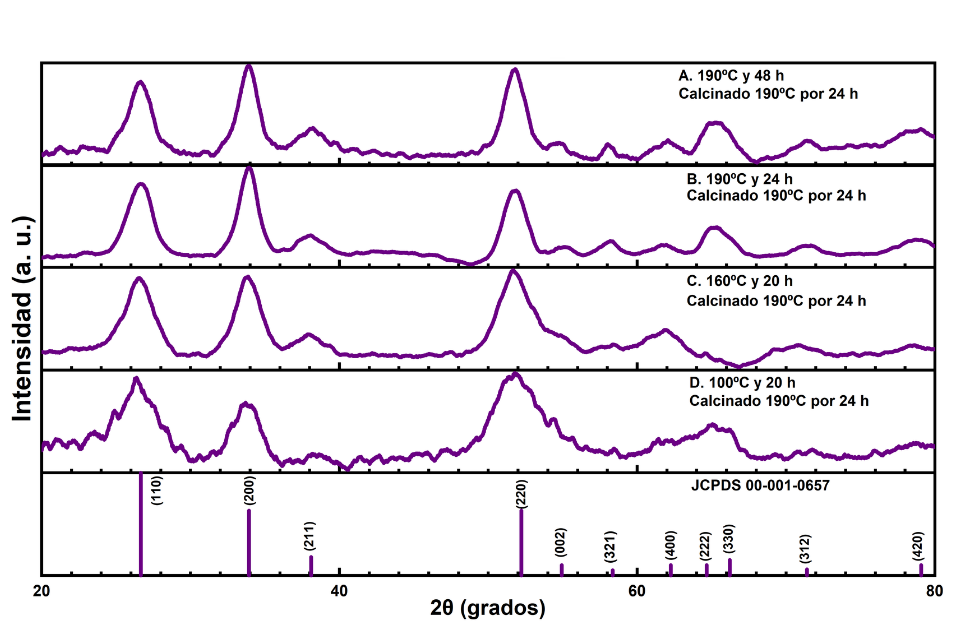
\includegraphics[width = 1\textwidth]{Imagenes/SnO2_Calcinado_ABCD.png}
     	  	\captionof{figure}{\label{fig:SnO2_Calcinado_ABCD}Patrón de difracción de rayos x del dióxido de estaño calcinado.} 
    	   \end{center} 
        \end{figure}


\begin{table}[h!]
\caption{Muestras de la Figura \ref{fig:SnO2_Calcinado_ABCD} y sus Características}
  \centering
  \begin{tabular}{|c|c|c|c|c|c|}
    \hline
    Muestra & Picos & Posición (x) & FWHM & Tamaño (nm) & Promedio (nm)\\
    \hline
    & (110) & 26.514 & 2.275 & 3.55 & \\
    A & (200) & 33.874 & 1.342 & 6.13 & \textcolor[rgb]{0.56,0.07,1}{3.385}\\
    & (220) & 43.327 & 17.611 & 0.48 & \\
    \hline
    & (110) & 26.622 & 2.013 & 4.01 & \\
    B & (200) & 33.881 & 1.715 & 4.79 & \textcolor[rgb]{0.56,0.07,1}{3.981}\\
    & (220) & 37.860 & 2.650 & 3.14 & \\
    \hline
    & (110) & 26.582 & 2.728 & 2.96 & \\
    C & (200) & 33.730 & 2.097 & 3.92 & \textcolor[rgb]{0.56,0.07,1}{2.946}\\
    & (220) & 52.019 & 4.462 & 1.96 & \\
    \hline
    & (110) & 26.568 & 2.761 & 2.93 & \\
    D & (200) & 33.832 & 2.341 & 3.51 & \textcolor[rgb]{0.56,0.07,1}{3.315}\\
    & (220) & 37.868 & 2.367 & 3.51 & \\
    \hline
  \end{tabular}
  \label{tab:drx2}
\end{table}


El tamaño cristalino se relaciona con la fotocatálisis porque entre menor sea el tamaño cristalino mayor será el área superficial. Esto significa que una mayor proporción de átomos o moléculas en la superficie del fotocatalizador están disponibles para interactuar con las moléculas objetivas en una reacción de fotocatálisis. Como resultado, hay más lugares activos para que ocurran las reacciones, lo que aumenta la eficiencia.\vspace{1em} % Espaciado adicional entre párrafos

Los cristales más pequeños tienden a reducir la recombinación de electrones y huecos, lo que es esencial para mantener una mayor eficiencia en la fotocatálisis. Cuanto más pequeño sea el cristal, menor será la probabilidad de que los electrones y huecos generados vuelvan a combinarse antes de participar en una reacción química.\vspace{1em} % Espaciado adicional entre párrafos

Sin embargo, es importante mencionar que el tamaño óptimo de los cristales depende del material y de la aplicación específica de la fotocatálisis. En algunos casos, los cristales demasiado pequeños pueden experimentar fenómenos de aglomeración o degradación de la eficiencia debido a la pérdida de ciertas propiedades.\vspace{1em} % Espaciado adicional entre párrafos

De acuerdo a lo anterior, se eligió la muestra C de la metodología de dióxido de estaño de la investigación \cite{IEEEreferencias:Ref36}, por ser la muestra con el tamaño cristalino más pequeño, lo que favorece la fotocatálisis. Con base en la muestra C propuse 4 muestras con una temperatura fija de 160 °C, con tiempo variado de 10, 20, 30 y 40 h, con un pH ácido de 3, una temperatura de secado de 60  °C por 5 h y una temperatura de calcinación de 190 °C por 24 h. Esto con el propósito de distinguir la influencia del tiempo en la síntesis hidrotermal y el tamaño cristalino más pequeño para el SnO$\displaystyle _{2}$. \vspace{1em} % Espaciado adicional entre párrafos

En la Figura \ref{fig:SnO2_Calcinado} las 4 muestras se etiquetaron como 10SnO$\displaystyle _{2}$, 20SnO$\displaystyle _{2}$, 30SnO$\displaystyle _{2}$ y 40SnO$\displaystyle _{2}$,de acuerdo al incremento en el tiempo se distingue que todas las muestras coinciden con los picos de la carta cristalográfica JCPDS 00-001-0657, también se percibe que los tres picos característicos con índices de Miller son (110), (200) y (220) y a partir de la ecuación de Scherrer se calcula el tamaño cristalino promedio como se indica en la Tabla \ref{tab:mi_drx3}. No se hace un promedio general, ya que eso nos podría incrementar el error. \vspace{1em} % Espaciado adicional entre párrafos

El tamaño promedio cristalino más pequeño es del 30SnO$\displaystyle _{2}$ con un valor de 2.64 nm, un microstrain de 4.86 y una densidad de dislocación de 146.27, al tener más defectos cristalinos en su red explicaría por qué no están bien definidos sus picos cristalinos.\vspace{1em} % Espaciado adicional entre párrafos

La muestra con los picos cristalinos más definidos es la muestra 40SnO$\displaystyle _{2}$ y la de 10SnO$\displaystyle _{2}$ con un valor promedio de 4.53 nm y 4.63 respectivamente, con un microstrain de 2.81 y 2.69, una densidad de dislocación con valor de 50.23 y 51.11, al ser las muestra con menos defectos cristalinos en su red explicaría por qué están bien definidos sus picos cristalinos.\vspace{1em} % Espaciado adicional entre párrafos

\begin{figure}[H]
    	   \begin{center}
     	  	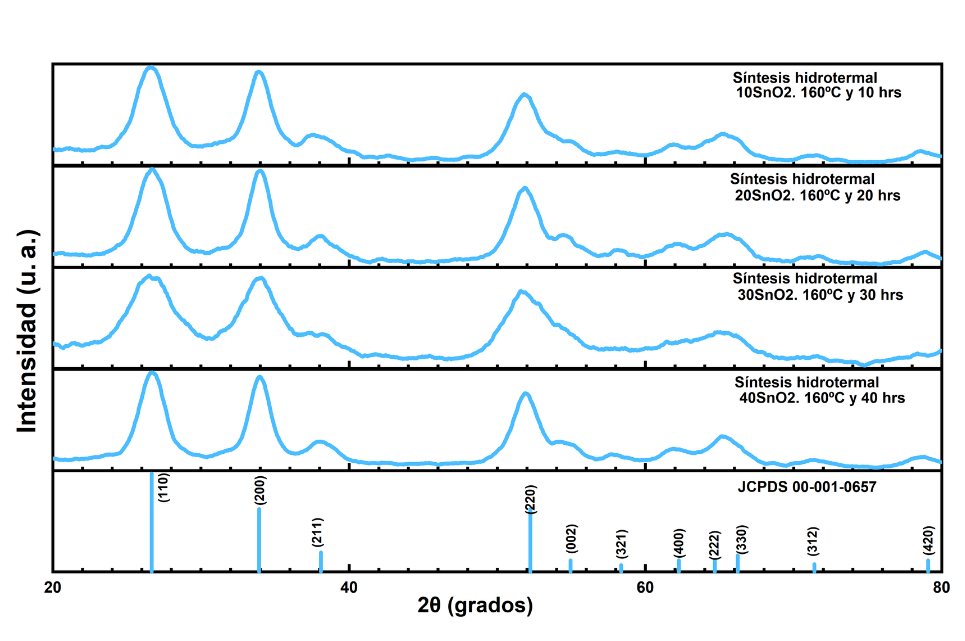
\includegraphics[width = 0.95\textwidth]{Imagenes/SnO2_Calcinado.png}
     	  	\captionof{figure}{\label{fig:SnO2_Calcinado}Patrón de difracción de rayos x del dióxido de estaño calcinado variando el tiempo y con temperatura fija. } 
    	   \end{center} 
        \end{figure}



\begin{table}[h!]
\caption{Muestras de la Figura \ref{fig:SnO2_Calcinado} y sus Características}
  \centering
  \begin{tabular}{|c|c|c|c|c|c|}
    \hline
    Muestra & Picos & Posición (x) & FWHM & Tamaño (nm) & Promedio (nm)\\
    \hline
    & (110) & 26.632300 & 2.22083 & 3.67 & \\
    10SnO$_{2}$ & (200) & 34.105800 & 1.812963 & 4.58 & \textcolor[rgb]{0.29,0.82,0.89}{4.63}\\
    & (220) & 52.176500 & 1.569875 & 5.64 & \\
    \hline
    & (110) & 26.701420 & 2.288577 & 3.56 & \\
    20SnO$_{2}$ & (200) & 34.152190 & 1.772355 & 4.69 & \textcolor[rgb]{0.29,0.82,0.89}{4.08}\\
    & (220) & 51.931260 & 2.206117 & 4.00 & \\
    \hline
    & (110) & 26.611550 & 3.311873 & 2.45 & \\
    30SnO$_{2}$ & (200) & 33.973890 & 2.831668 & 2.92 & \textcolor[rgb]{0.29,0.82,0.89}{2.64}\\
    & (220) & 52.125670 & 3.46708 & 2.54 & \\
    \hline
    & (110) & 26.698090 & 1.989464 & 4.06 & \\
    40SnO$_{2}$ & (200) & 33.979650 & 1.588004 & 5.17 & \textcolor[rgb]{0.29,0.82,0.89}{4.53}\\
    & (220) & 51.985120 & 2.004494 & 4.36 & \\
    \hline
  \end{tabular}
  \label{tab:mi_drx3}
\end{table}

 Sin embargo, para una caracterización detallada del decorado, se requiere un análisis más específico que puede incluir técnicas adicionales, como UV-VIS, Raman, FTIR, para determinar la composición elemental de la muestra decorada.
 

\subsubsection{UV-vis}

Los espectros de absorbancia UV-Vis de las nanopartículas de 10SnO$\displaystyle _{2}$, 20SnO$\displaystyle _{2}$, 30SnO$\displaystyle _{2}$ y 40SnO$\displaystyle _{2}$ se muestran en la  Figura \ref{fig:tt}. 
Generalmente, las nanopartículas semiconductoras se someten a un confinamiento cuántico que depende del tamaño. La banda prohibida de los materiales aumenta cuando el tamaño de las partículas disminuye y el borde de absorción se desplaza hacia el lado de mayor energía.\vspace{1em} % Espaciado adicional entre párrafos

En consecuencia, en el presente trabajo, el pico de absorción observado de las 4 muestras de la gráfica de "Dióxido de Estaño" es a 300 nm para las nanopartículas de SnO$\displaystyle _{2}$. Para las partículas de 1GO hay un corrimiento a la derecha, lo que indica un desplazamiento hacia el rojo. La banda prohibida se calcula usando la ecuación \ref{eq:ecu4}, donde toma el valor de dos para una transición directa permitida, A es una constante llamada parámetro de cola de bandas, y h es la fotoenergía incidente.
\vspace{1em} % Espaciado adicional entre párrafos

La banda prohibida directa se estimó utilizando Tauc plot con ayuda del software Origin 2023, que se traza entre hm y (ahm)2. La Figura \ref{fig:tt}  muestra la banda prohibida de las nanopartículas de 10SnO$\displaystyle _{2}$, 20SnO$\displaystyle _{2}$, 30SnO$\displaystyle _{2}$, 40SnO$\displaystyle _{2}$ y las de óxido de grafeno decorado con SnO$\displaystyle _{2}$, 1GO, 2.5GO, 5GO, 10GO. La banda prohibida directa de las nanopartículas 10SnO$\displaystyle _{2}$, 20SnO$\displaystyle _{2}$, 30SnO$\displaystyle _{2}$, 40SnO$\displaystyle _{2}$ es 3.530, 2.575, 3.201 y 2.642 eV, respectivamente.

\begin{figure}[H]
    	   \begin{center}
     	  	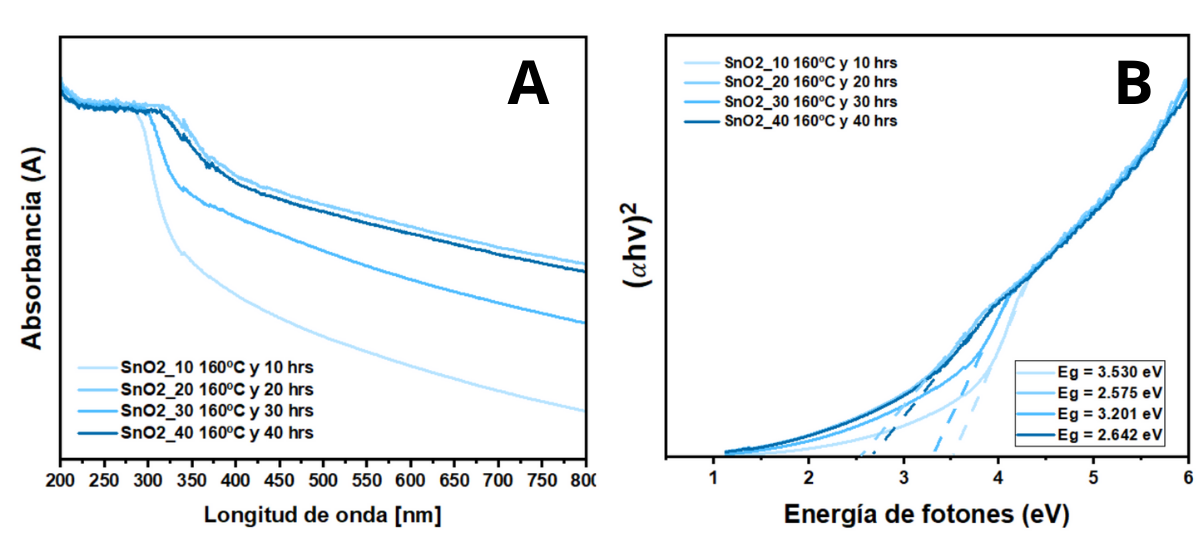
\includegraphics[width = 1\textwidth]{Imagenes/tt.png}
     	  	\captionof{figure}{\label{fig:tt}A, espectro de absorbancia en UV del dióxido de estaño en sus 4 diferentes temperaturas. B, el cálculo del Band Gap por el método de Tauc Plot. } 
    	   \end{center} 
        \end{figure}

\subsubsection{FTIR}

El espectro de FTIR del dióxido de estaño después de tratarlo a una temperatura fija de 160 ºC y un tiempo variable de 10, 20, 30 y 40 h. En la  Figura \ref{fig:SnO2_FTIR_2} la fuerte vibración que se extiende de 500 a 4000 cm$\displaystyle ^{-1}$ indica la presencia de enlaces de hidrógeno involucrados en O- H, derivados del agua adsorbida y grupos Sn-OH.\vspace{1em} % Espaciado adicional entre párrafos

En el citrato sólido, los grupos carboxilo son ionizados, por lo que el pico de 1538 cm$\displaystyle ^{-1}$ se puede asignar a vibración del grupo COO del complejo de citrato, entre el pico a 1716 cm$\displaystyle ^{-1}$ probablemente corresponde al COOR, causados por cloro. Los picos entre 1118 y 900 cm-1 se atribuyen a la vibración de enlaces hidroxilo-estaño. La vibración en 424 \ cm$\displaystyle ^{-1}$ está relacionada con la vibración del oxígeno terminal de Sn-OH y el pico a 603 y 796 cm$\displaystyle ^{-1}$ es atribuible a los grupos funcionales puente OXO (OSnO).
\begin{figure}[H]
    	   \begin{center}
     	  	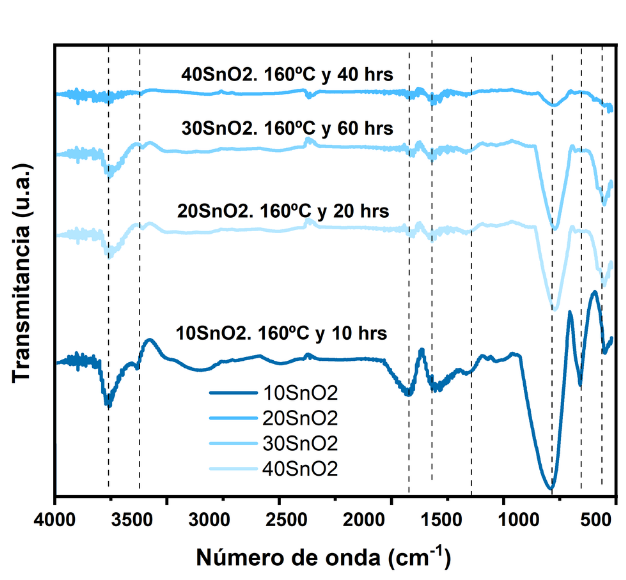
\includegraphics[width = 1\textwidth]{Imagenes/SnO2_FTIR_2.png}
     	  	\captionof{figure}{\label{fig:SnO2_FTIR_2}Espectro en FTIR de dióxido de estaño calcinado variando el tiempo de reacción de 10-40 h.} 
    	   \end{center} 
        \end{figure}


\begin{table}[h!]
\centering
\caption{Modos vibracionales característicos de diferentes grupos químicos del SnO.}
\begin{tabular}{|c|c|c|}
\hline
\textbf{Grupo Químico} & \textbf{Modo Vibracionales} & \textbf{Número de Onda} (\(\text{cm}^{-1}\)) \\ \hline
COO                    & Tensión simétrica         & 1538                                         \\ \hline
COOR                   & Tensión simétrica         & 1716                                         \\ \hline
Sn-OH                  & Tensión simétrica         & 118-900                                     \\ \hline
OXO (OSnO)             & Tensión simétrica         & 603 y 796                                   \\ \hline
\end{tabular}

\label{tab:grupos_quimicos}
\end{table}
        
\subsubsection{RAMAN}
En la espectroscopia de RAMAN de pared simple es posible distinguir si el material es semiconductor o metálico debido a la quiralidad, esto quiere decir que el material cuenta con la característica de no ser superponible con su imagen especular (mano izquierda sobre mano derecha). Es muy útil para identificar heteroátomos de tipo n o p y poder describir la estructura, número de láminas, la calidad y los defectos que se presenten en la muestra en polvo, en este caso.\vspace{1em} % Espaciado adicional entre párrafos

 Es bien sabido que la estructura tetragonal del rutilo SnO$\displaystyle _{2}$ tiene seis átomos (dos Sn y cuatro iones O) en cada celda unitaria, y los modos de vibración de la red normal.  
Los modos activos Raman de B1g, Eg, A1g y B2g están permitidos en rutilo SnO$\displaystyle _{2}$ con el punto grupo de DI4 4h y el grupo espacial de P42/mnm [4]. La Figura \ref{fig:RAMAN_SnO2_2} muestra los espectros de dispersión Raman de los productos tal como están preparados. Los picos ubicados en 134.191, 632.787 y 771.778 cm$\displaystyle ^{-1}$ corresponder a las vibraciones B1g, Eg, A1g y B2g, respectivamente.\vspace{1em} % Espaciado adicional entre párrafos

Esto confirma que el producto preparado es el rutilo tetragonal SnO$\displaystyle _{2}$. Además, una amplia y fuerte pico en 570,607 cm$\displaystyle ^{-1}$ y un pico débil en 303,482 cm$\displaystyle ^{-1}$ se observa en los espectros. Se ha demostrado que no son los modos activos Raman de rutilo tetragonal SnO$\displaystyle _{2}$ y no se puede observar en general. Que se observen aquí puede estar relacionado con el área de la superficie facetaria de las nanohojas, que son causadas por el efecto de tamaño pequeño de las nanopartículas.\vspace{1em} % Espaciado adicional entre párrafos


Además, un nuevo pico de 401 cm$\displaystyle ^{-1}$ también se detecta en los espectros. Aunque este modo vibratorio necesita más estudios, se cree que se atribuye a la reducción del tamaño de las nanopartículas o a la alta concentración de defectos superficiales, como vacantes de oxígeno según la relajación del Raman la regla de selección. Como conjetura, el pequeño tamaño y los defectos superficiales de las nanoláminas de SnO$\displaystyle _{2}$ pueden ser un efecto positivo en fotocatálisis.

        \begin{figure}[H]
    	   \begin{center}
     	  	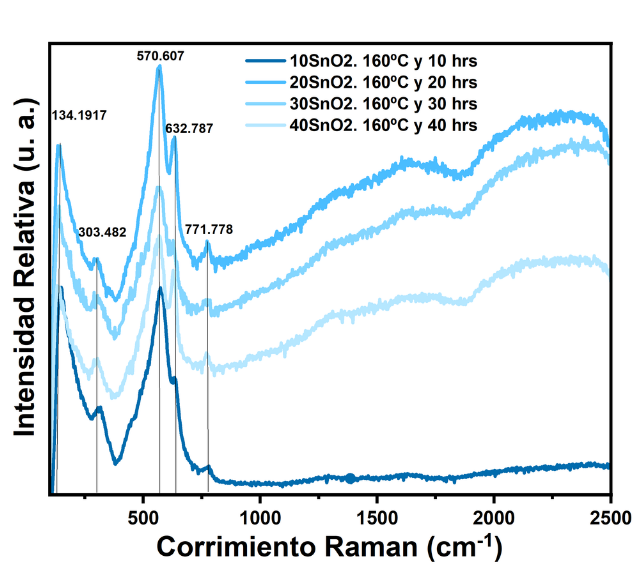
\includegraphics[width = 1\textwidth]{Imagenes/RAMAN_SnO2_2.png}
     	  	\captionof{figure}{\label{fig:RAMAN_SnO2_2}Espectro RAMAN del  dióxido de estaño con la la temperatura fija y sus 4 variaciones de temperatura.} 
    	   \end{center} 
        \end{figure}
        
        \begin{table}[h!]
        \centering
        \caption{Frecuencias de modos vibracionales para muestras de SnO\(_{2}\).}
        \begin{tabular}{|c|c|c|c|c|}
        \hline
        \textbf{Muestra}   & \(\mathbf{B_{1g}}\) & \(\mathbf{E_{U}}\) & \(\mathbf{A_{2g}}\) & \(\mathbf{A_{1g}}\) \\ \hline
        10SnO\(_{2}\)     & 134.1917           & 303.482           & 570.607            & 771.778            \\ \hline
        20SnO\(_{2}\)     & 134.1917           & 303.482           & 570.607            & 771.778            \\ \hline
        30SnO\(_{2}\)     & 134.1917           & 303.482           & 570.607            & 771.778            \\ \hline
        40SnO\(_{2}\)     & 134.1917           & 303.482           & 570.607            & 771.778            \\ \hline
        \end{tabular}
        
        \label{tab:modos_snO2}
        \end{table}


\subsubsection{SEM} 
En la imagen SEM de la Figura \ref{fig:SEM_SnO2}, no se perciben claramente las nanoesferas individuales debido a las limitaciones de resolución, pero se distinguen aglomerados de nanoesferas con un tamaño aproximado de 1 µm. Estos aglomerados aparecen como estructuras compactas y distribuidas de manera uniforme sobre la superficie del material, indicando que las nanoesferas tienden a formar cúmulos a esa escala. La morfología general de estos aglomerados sugiere una interacción entre las nanoesferas, lo que genera la formación de estas agrupaciones visibles.
        \begin{figure}[H]
    	   \begin{center}
     	  	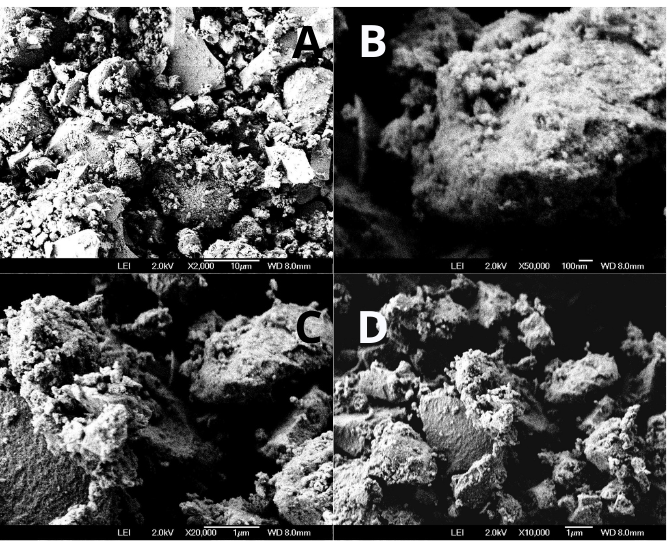
\includegraphics[width = 1\textwidth]{Imagenes/SEM_SnO230.png}
     	  	\captionof{figure}{\label{fig:SEM_SnO2}Microscopia electrónica de barrido del dióxido de estaño para las cuatro muestras: A para 10SnO2, B para 20SnO2, C para 30SnO2 y D para 40SnO2.} 
    	   \end{center} 
        \end{figure}

        
\subsection{Discusión y análisis de resultados del SnO$\displaystyle _{2}$@GO}


Se repetirá la metodología de acuerdo al material con mejores condiciones de tiempo, pH y temperatura para los catalizadores decorados de SnO$\displaystyle _{2}$@GO, haciendo diferentes concentraciones en el medio de reacción para molaridades de 0.1, 0.2, 0.4 y 1 M se llevará a pruebas de caracterización de DRX, UV-vis, FTIR, Raman, XPS y SEM para identificar sus características fotocataliticas y ponerlos a prueba ante los colorantes de AM y R6G.\vspace{1em} % Espaciado adicional entre párrafo

\subsubsection{DRX} 

 El cambio en la concentración del medio de reacción (agua y etanol) afecta significativamente el proceso de nucleación y crecimiento de las nanopartículas de SnO$\displaystyle _{2}$  en el nanocompuesto SnO$\displaystyle _{2}$@GO. Las condiciones de síntesis alteran el tamaño cristalino, lo que se refleja en el ensanchamiento o estrechamiento de los picos en los espectros de DRX de la Figura \ref{fig:SnO2@GO}. Las proporciones adecuadas de agua y etanol controlan la morfología y la dispersión de las nanopartículas, optimizando la interacción con el GO y, por lo tanto, la eficiencia fotocatalítica del material.

 \begin{figure}[H]
    	   \begin{center}
     	  	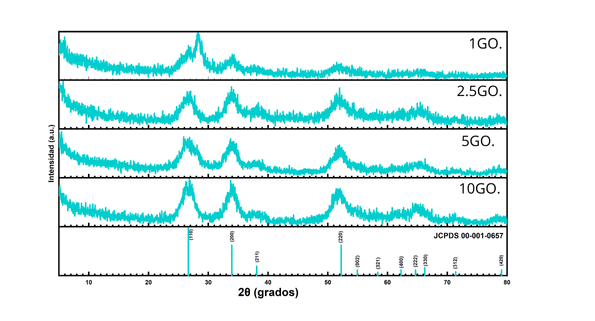
\includegraphics[width = 1.1\textwidth]{Imagenes/SnO2_decorado_xrd.png}
     	  	\captionof{figure}{\label{fig:SnO2@GO}Patrón de difracción de rayos x del óxido de grafeno decorado con dióxido de estaño, variando la concentración del medio de reacción del dióxido de estaño. } 
    	   \end{center} 
        \end{figure}
 
\begin{table}[h!]
\centering
\caption{Materiales de SnO$\displaystyle _{2}$@GO.}
\begin{tabular}{|c|c|c|c|c|c|}
\hline
Muestra & Miller & (x) & FWHM & Tamaño & Promedio \\ \hline
1GO & (110) & 28.392 & 8.312 & 0.95 & \multirow{3.47} \\
    & (200) & 33.945 & 1.340 & 6.05 &  \\
    & (220) & 52.071 & 2.412 & 3.40 &  \\ \hline
2.5GO & (110) & 26.593 & 2.226 & 3.63 & \multirow{3.41} \\
      & (200) & 34.047 & 2.210 & 3.72 &  \\
      & (220) & 52.052 & 3.029 & 2.89 &  \\ \hline
5GO & (110) & 26.708 & 3.148 & 2.56 & \multirow{3.05} \\
    & (200) & 33.987 & 2.383 & 3.45 &  \\
    & (220) & 52.971 & 2.793 & 3.13 &  \\ \hline
10GO & (110) & 26.617 & 2.392 & 3.37 & \multirow{3.36} \\
     & (200) & 33.937 & 2.162 & 3.80 &  \\
     & (220) & 52.028 & 3.021 & 2.89 &  \\ \hline
\end{tabular}
\label{table:go_decorado }
\end{table}
\newpage

\subsubsection{UV-vis}
Para SnO$\displaystyle _{2}$@GO su banda prohibida directa de las nanopartículas 1GO, 2.5GO, 5GO, 10GO,  es 4.883, 4.429, 3.461, 3.733 eV respectivamente. De la literatura se desprende que al disminuir la banda prohibida está asociado con una disminución en el tamaño de las partículas, lo cual es bueno, ya que de acuerdo a la literatura el band gap del SnO$\displaystyle _{2}$ es de 3.6 eV y en la prueba 5GO se disminuyo como se observa en la Figura \ref{fig:UV_SNOGO}.  \cite{IEEEreferencias:Ref36}.
\begin{figure}[H]
    	   \begin{center}
     	  	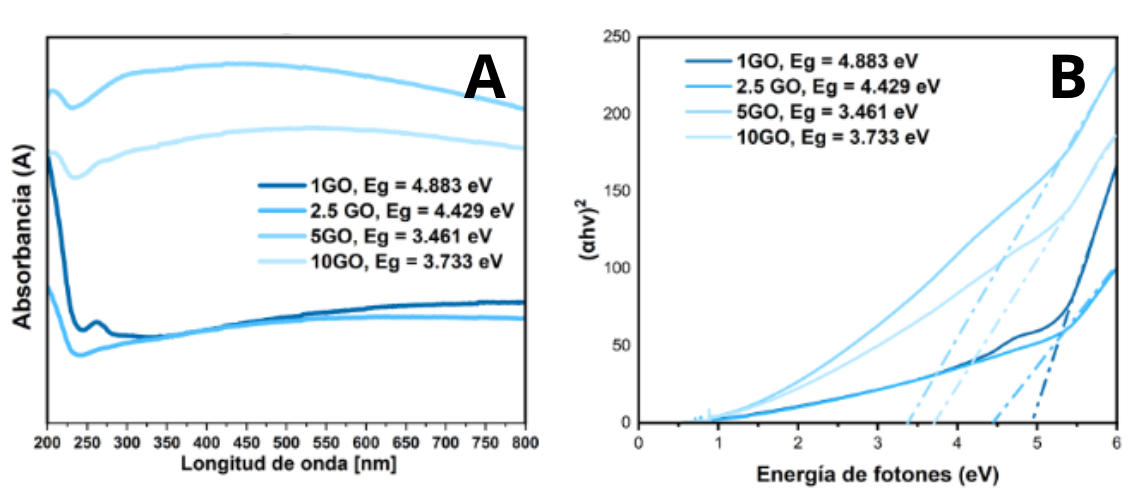
\includegraphics[width = 1\textwidth]{Imagenes/UV_SNOGO.png}
     	  	\captionof{figure}{\label{fig:UV_SNOGO}A, espectro de absorbancia en UV del óxido de grafeno decorado con dióxido de estaño variando la temperatura de 10 a 30 h. B, el cálculo del Band Gap por el método de Tauc Plot. } 
    	   \end{center} 
        \end{figure}
    

\subsubsection{FTIR}
De acuerdo al espectro de FTIR de SnO$\displaystyle _{2}$@GO de la Figura \ref{fig:FTIR_SnO2} se identificaron los siguientes grupos funcionales de GO de la Tabla \ref{tab:modos_GO_SnO2}: 
Grupo hidroxilo (OH): Una banda ancha alrededor de 3200-3600 cm$\displaystyle ^{-1}$ debido a las vibraciones de estiramiento de los grupos hidroxilo (OH) adsorbidos o ligados a la superficie del GO.
Estiramiento C=O: Una banda fuerte alrededor de 1720 cm$\displaystyle ^{-1}$, correspondiente a los grupos carbonilo (C=O) de los ácidos carboxílicos o cetonas.
Estiramiento C=C: Una banda en torno a 1620 cm$\displaystyle ^{-1}$, relacionada con las vibraciones de los enlaces dobles carbono-carbono en el esqueleto de grafeno.
Estiramiento C-O-C y C-OH: Bandas entre 1000 y 1300 cm$\displaystyle ^{-1}$, que indican la presencia de epóxidos y alcoholes (C-O-C y C-OH, respectivamente).\vspace{1em} % Espaciado adicional entre párrafos

Cuando se realiza una síntesis hidrotermal de SnO$\displaystyle _{2}$ y GO, es posible observar cambios en el espectro FTIR debido a la interacción entre estos dos materiales:\vspace{1em} % Espaciado adicional entre párrafos

Modificaciones en las bandas de SnO$\displaystyle _{2}$: La presencia de GO puede inducir cambios en las bandas características de SnO$\displaystyle _{2}$, especialmente si hay formación de enlaces entre SnO$\displaystyle _{2}$ y los grupos funcionales del GO. Esto puede resultar en desplazamientos de las bandas de Sn-O o la aparición de nuevas bandas.\vspace{1em} % Espaciado adicional entre párrafos

Reducción de grupos oxigenados en GO: Durante la síntesis hidrotermal, el GO puede sufrir una reducción parcial, disminuyendo la intensidad de las bandas relacionadas con los grupos oxigenados (OH, C=O, C-O-C, C-OH) y aumentando la intensidad de la banda de C=C, lo cual indica una recuperación parcial de la estructura de grafeno.\vspace{1em} % Espaciado adicional entre párrafos

Nuevas interacciones: La formación de enlaces químicos o interacciones fuertes entre SnO$\displaystyle _{2}$ y GO puede resultar en nuevas bandas en el espectro FTIR. Estas bandas pueden aparecer en la región de 1000-1600 cm$\displaystyle ^{-1}$, donde los modos de vibración de los grupos funcionales oxigenados pueden acoplarse con las vibraciones de SnO$\displaystyle _{2}$.

\begin{figure}[H]
    	   \begin{center}
     	  	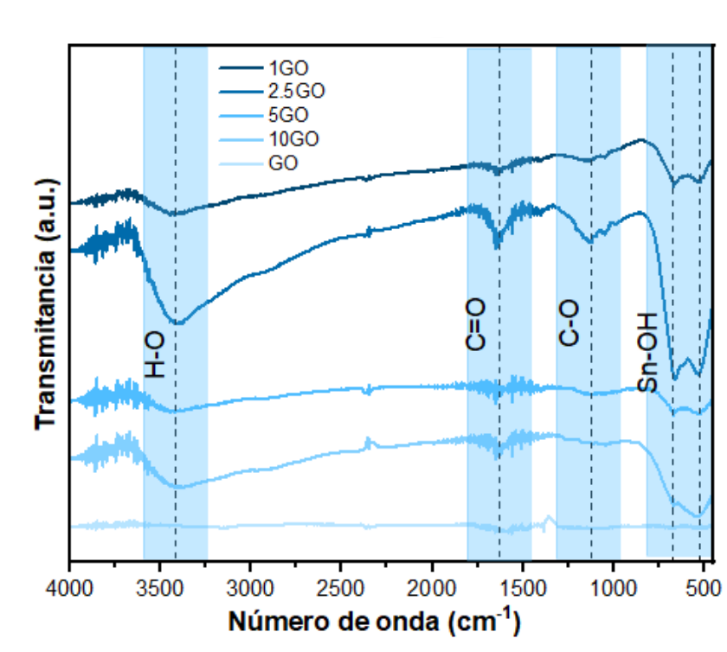
\includegraphics[width = 0.7\textwidth]{Imagenes/SnO2@GO_FTIR_2.png}
     	  	\captionof{figure}{\label{fig:FTIR_SnO2}Espectro en FTIR del óxido de grafeno decorado con dióxido de estaño.} 
    	   \end{center} 
        \end{figure}

\begin{table}[h!]
\centering
\caption{Modos vibracionales de grupos químicos en GO y SnO\(_2\).}
\begin{tabular}{|l|c|c|}
\hline
\textbf{Grupo Químico}                   & \textbf{Modo Vibracional} & \textbf{Número de Onda} (\(\text{cm}^{-1}\)) \\ \hline
\multirow{Óxido de Grafeno (GO)}   & C-O, C=O,C=O, C-O-C, C-OH,C=C                  & 1130, 1650                                   \\ \cline{2-3} 
                                         & Tensión simétrica         &                                              \\ \hline
\multirow{Dióxido de Estaño (SnO\(_2\))} & Sn-OH                   & 530-669                                     \\ \cline{2-3} 
                                         & Tensión simétrica         &                                              \\ \hline
\end{tabular}
\label{tab:modos_GO_SnO2}
\end{table}


        
\subsubsection{RAMAN}

La singularidad de Van Hove del GO en los espectros RAMAN se pueden distinguir claramente en la Figura \ref{fig:RAMAN_AZUL} y puntualmente en la Tabla \ref{tab:Raman_SnOGO}, en donde los espectros fotónicos del SnO$\displaystyle _{2}$@GO que se perciben alrededor de 1600 cm$\displaystyle ^{-1}$, esta banda pertenece a la vibración de primer orden o fundamental conocida como banda grafítica (G+) que pertenece al GO.\vspace{1em} % Espaciado adicional entre párrafos


Para grafito policristalino se distingue una banda situada aproximadamente en 1350 cm$\displaystyle ^{-1}$ conocida como D o de desorden inducido que se involucra fonones de segundo orden. Esta banda nos indica defectos en la red cristalina y por ende de su calidad \cite{IEEEreferencias:GORAMAN}.\vspace{1em} % Espaciado adicional entre párrafos

La relación de intensidad (ID/IG) de la banda D a la banda G es relacionado con la extensión del grado de trastorno y el tamaño promedio del sp2 dominios. La intensidad del valor de ID/IG para 1GO, 2.5GO, 5GO y 10GO es de 0.8415, 0.84531, 0.8415 y 0.83609 respectivamente. Lo que significa que la concentración en el GO es constante en cada catalizador.\vspace{1em} % Espaciado adicional entre párrafos

\begin{figure}[H]
    	   \begin{center}
     	  	\includegraphics[width = 0.8\textwidth]{Imagenes/SnO2GO_RAMAN.png}
     	  	\captionof{figure}{\label{fig:RAMAN_AZUL}Espectro RAMAN del óxido de grafeno decorado con dióxido de estaño, donde se visualiza la banda D y G.} 
    	   \end{center} 
        \end{figure}
\begin{table}[ht]
    \centering
    \caption{Corrimiento RAMAN de las bandas características de SnO$\displaystyle _{2}$@GO}
    \begin{tabular}{|c|c|c|c|c|c|}
        \toprule
        \hline
        Muestra & D & G & Eg & B2g \\
        \midrule
        \hline
        1GO & 1348.814 & 1602.872 & 483.362 & 632.788 \\ \hline
        2.5GO & 1348.814 & 1595.651 & 483.362 & 632.788 \\\hline
        5GO & 1348.814 & 1602.872 & 483.362 & 632.788 \\\hline
        10GO & 1346.333 & 1610.277 & 483.362 & 632.788 \\\hline
        GO & 1348.814 & 1588.423 & N/A & N/A \\\hline
        \bottomrule
    \end{tabular}
    \label{tab:Raman_SnOGO}
\end{table}

\subsubsection{XPS}
Los espectros XPS se realizaron en el Centro de Nanociencias y Micro y Nanotecnologías con el equipo de la Figura \ref{fig:EquipoXPS}, para estudiar la composición química y el estado de valencia de la superficie de los 4 nanomateriales de SnO$\displaystyle _{2}$@GO en polvo.\vspace{1em} % Espaciado adicional entre párrafos

Los espectros medidos se descompusieron en componentes gaussianos con antecedentes de Shirley usando Origin 2024. La Figura \ref{fig:XPS_SNOGO1} muestra los espectros de C1s, Sn 3d y O 1s del polvo de SnO$\displaystyle _{2}$@GO, respectivamente. La Figura \ref{fig:XPS_SNOGO2}E de Sn3d muestra los espectros XPS simétricos de alta resolución, en donde los picos de división del doblete clásico 3d3/2–3d5/2 da un valor en promedio de 495.18 y 486.7325 eV se pueden asignar a la red de estaño en SnO$\displaystyle _{2}$.\vspace{1em} % Espaciado adicional entre párrafos


\begin{figure}[H]
    	   \begin{center}
     	  	\includegraphics[width = 0.85\textwidth]{Imagenes/XPS_SNOGO1.png}
     	  	\captionof{figure}{\label{fig:XPS_SNOGO1}Espectro de XPS de los cuatro catalizadores decorados de SnO$\displaystyle _{2}$@GO.} 
    	   \end{center} 
        \end{figure}

Los 8,4475 eV de la diferencia de energía entre Sn 3d5/2 y Sn 3d3/2 están en buen estado de acuerdo con la división de energía reportada para SnO$\displaystyle _{2}$. El pico de Sn 3d5/2 es muy consistente con los datos estándar de SnO$\displaystyle _{2}$ (486,70 eV), lo que indica que el Sn está presente en un estado químico de +4. \vspace{1em} % Espaciado adicional entre párrafos

El espectro XPS de escaneo estrecho de los O1s demuestra las características amplias y asimétricas, lo que sugiere varias coordinaciones de oxígeno en las nanopartículas. El pico de O1s, que se observa en la Figura \ref{fig:XPS_SNOGO2}F, se puede convertir cuidadosamente en tres picos simétricos ubicados en 530.76, 532.28 y 533.536 eV respectivamente, lo que indica la presencia de tres tipos de especies de oxígeno en las nanohojas. \vspace{1em} % Espaciado adicional entre párrafos

El pico centrado en 530,725 eV se asigna a iones de oxígeno en la roja cristalina de SnO$\displaystyle _{2}$ (red de O) en condiciones estequiométricas completamente oxidadas. Los picos ubicados en 532,280 eV se pueden atribuir al oxígeno defectuoso causado por la vacante de oxígeno (VO), el oxígeno intersticial (Oi) y el antisitio de oxígeno (OSn), lo que sugiere una alta concentración de huecos dentro de la región con deficiencia de oxígeno. Esos agujeros pueden favorecer la absorción de oxígeno de la atmósfera.\vspace{1em} % Espaciado adicional entre párrafos

El pico ubicado en 533,556 eV proviene de las especies Ox absorbidas (iones O u O2), lo que indica que especies ricas en oxígeno se adsorbieron en la superficie de las nanohojas de SnO$\displaystyle _{2}$. Por lo tanto, el aumento de iones de oxígeno adsorbidos puede promover la fotocatálisis del SnO$\displaystyle _{2}$@GO.\vspace{1em} % Espaciado adicional entre párrafos

El pico C1s Figura \ref{fig:XPS_SNOGO2}D, se subdividió en cuatro picos individuales después del ajuste del pico principal. Se observó que los picos a 284, 286, 287 y 288 eV correspondían a C-C/C=C, C-O, C=O y O-C=O, respectivamente, como se muestra en un estudio anterior. Estos resultados revelan que el GO tenía un grupo de oxígeno residual.

\begin{figure}[H]
    	   \begin{center}
     	  	\includegraphics[width = 1\textwidth]{Imagenes/XPS_SNOGO2.png}
     	  	\captionof{figure}{\label{fig:XPS_SNOGO2}Espectro de XPS de los cuatro catalizadores decorados de SnO$\displaystyle _{2}$@GO.} 
    	   \end{center} 
        \end{figure}

        
\subsubsection{SEM}

En la microscopia electrónica de barrido del óxido de grafeno decorado con dióxido de estaño para las cuatro muestras: 10GO, 5GO, 2.5GO Y 1GO, de la Figura \ref{fig:SEM_SnO2GO}. Destaca la imagen del catalizador de 10GO, debido a que se visualizan las nanoesferas del semiconductor de SnO$\displaystyle _{2}$ sobre las capas de GO que se distinguen más oscuras. La imagen muestra cómo el GO evita que se aglomeren las nanoesferas para que exista una mayor área superficial que esté en contacto con el colorante. Los otros catalizadores no presentan las nanoesferas debido a que eran poco GO y solo se distinguen aglomeraciones del SnO$\displaystyle _{2}$, que forman cúmulos de distintas dimensiones. Estos cúmulos aparecen como regiones brillantes debido a su naturaleza metálica y densa, en contraste con el GO, que se manifiesta como áreas más oscuras y dispersas.

\begin{figure}[H]
    	   \begin{center}
     	  	\includegraphics[width = 0.85\textwidth]{Imagenes/SEM_SnO2GO.png}
     	  	\captionof{figure}{\label{fig:SEM_SnO2GO}Microscopia electrónica de barrido del óxido de grafeno decorado con dióxido de estaño para las cuatro muestras: 10GO, 5GO, 2.5GO Y 1GO.} 
    	   \end{center} 
        \end{figure}
\subsection{Discusión y análisis de resultados del ZnO}
Una vez obtenidos, los catalizadores en polvo se caracterizarán por DRX, UV-vis y RAMAN, para identificar sus características fotocatalíticas como menor banda ancha, el de tamaño cristalino más pequeño y el de mayor presencia de grupos funcionales oxigenados. 
 \subsubsection{DRX}
 Todas las muestras de ZnO se caracterizaron con la técnica de difracción de rayos x con el equipo del CICQS Difractómetro de rayos X Bruker D8 Advance LinxEye, con condiciones de 2θ de 20° a 80°, 30 kV, 25 mA, 0.03°/paso, 0.3 s/paso. Fuente de rayos X: Tubo de descarga con ánodo de cobre (Kα1 = 0.1540 Å). El tipo de detector fue unidimensional (LinxEye fast speed) con área activa de 14 mm x 16 mm y eficiencia del 0.98.

Para el estudio de un semiconductor que funcione como fotocatalizador capaz de acelerar la reacción  se replicó la investigación de óxido de zinc (ZnO) por síntesis hidrotermal, donde se utilizó como precursor él $\displaystyle Zn( CH_{3} COO)_{2} \smblkcircle 2H_{2}O$  y con una variación en el reductor NaOH, dependiendo el pH alcalino del 9 al 13. Para el uso de la autoclave se siguió la metodología para las 4 muestras etiquetadas como A, B, C, D y E, todas las muestras sometidas a las mismas condiciones de temperatura y tiempo de 120 °C por 4.5 h.\vspace{1em} % Espaciado adicional entre párrafos

Para describir las cinco muestras de ZnO de la Figura \ref{fig:ZnO_DRX_1} sintetizadas bajo valores de 13, 12, 11, 10 y 9 de pH, con tamaños promedio de cristal de 28.565 nm, 27.178 nm, 21.415 nm, 37.004 nm y 31.073 nm respecto a la Tabla \ref{tab:zno1DRX}, podemos hacer una interpretación del efecto del pH en el tamaño de cristal y las posibles características estructurales que se observan a través de técnicas como Difracción de Rayos X (DRX) para identificar la muestra de ZnO con el tamaño de cristal más pequeño para decorar el GO.\vspace{1em} % Espaciado adicional entre párrafos


Con ayuda del software Origin 2023, se graficaron los espectros de DRX del ZnO y se calculó con la ecuación \ref{eq:ecu3} de Scherrer el tamaño promedio de los cristalitos con los tres picos característicos que se encuentran en los índices de Miller (100), (002) y (101) de acuerdo a la carta cristalográfica JCPDS 00-0079-2205, que corresponde al óxido de zinc con una estructura cristalina de wurtzita.

Se puede distinguir que a medida que se disminuye el pH de 13 a 9 en la Tabla \ref{tab:zno1DRX}, se observa una variabilidad en el tamaño de cristal, lo que refleja cómo las condiciones de síntesis, en especial la concentración de iones OH⁻, afectan tanto la nucleación como el crecimiento de los cristales de ZnO.\vspace{1em} % Espaciado adicional entre párrafos

El ancho de los picos de DRX debería correlacionarse con el tamaño de cristal. Los materiales con tamaños de cristal más pequeños (como en pH 11) tendrán picos más anchos, mientras que los de mayor tamaño de cristal (como en pH 10) tendrán picos más estrechos \cite{IEEEreferencias:Scherrer}.
Los tamaños de cristal más pequeños a pH 11 sugieren la presencia de más defectos estructurales, mientras que los tamaños de cristal más grandes en pH 10 y 9 indican una mejor cristalinidad y menor cantidad de defectos.\vspace{1em} % Espaciado adicional entre párrafos

Las muestras sintetizadas bajo diferentes pH presentan una variabilidad en el tamaño del cristal, con tamaños menores a pH 11 (21.415 nm) y mayores a pH 10 (37.004 nm). A medida que el pH disminuye, el crecimiento cristalino parece estar influenciado por la cantidad de iones OH⁻, lo que afecta tanto la nucleación como el crecimiento. Los tamaños de cristal mayores (en pH 10 y 9) indican alta cristalinidad, mientras que los tamaños más pequeños (en pH 11) sugieren la presencia de defectos y menor orden estructural.\vspace{1em} % Espaciado adicional entre párrafos


Se elegiría un pH de 11 para la fotocatálisis porque proporciona un tamaño de cristal más pequeño y, por lo tanto, una mayor área superficial para reacciones fotocatalíticas, mejora la generación de radicales hidroxilo, y mantiene la estabilidad estructural del ZnO en un medio ligeramente alcalino. Además, este pH favorece la adsorción de ciertos contaminantes y permite que el ZnO conserve su capacidad catalítica sin comprometer su integridad durante el proceso fotocatalítico.

\begin{figure}[H]
    	   \begin{center}
     	  	\includegraphics[width = 0.77\textwidth]{Imagenes/ZnO_DRX_1.png}
     	  	\captionof{figure}{\label{fig:ZnO_DRX_1}Patrón de difracción de rayos x del óxido de zinc variando valores de pH de 9 a 13.  } 
    	   \end{center} 
        \end{figure}

\begin{table}[h]
\caption{Resultados de diferentes muestras con sus correspondientes picos, posiciones, FWHM, tamaños y promedios.}
\centering
\begin{tabular}{|c|c|c|c|c|c|}
\hline
\textbf{Muestra} & \textbf{Picos} & \textbf{Posición (x)} & \textbf{FWHM} & \textbf{Tamaño (nm)} & \textbf{Promedio (nm)} \\ \hline
 & (100) & 32.029 & 0.281 & 31.24 &  \\
\textbf{13pH} & (002) & 34.683 & 0.269 & 32.94 & \textcolor[rgb]{0.29,0.56,0.89}{28.565} \\
 & (101) & 36.479 & 0.404 & 21.52 &  \\ \hline
 & (100) & 31.920 & 0.324 & 26.87 &  \\
\textbf{12pH} & (002) & 34.560 & 0.294 & 29.93 & \textcolor[rgb]{0.29,0.56,0.89}{27.178} \\
 & (101) & 36.402 & 0.354 & 24.73 &  \\ \hline
 & (100) & 31.866 & 0.449 & 19.04 &  \\
\textbf{11pH} & (002) & 34.521 & 0.327 & 26.78 & \textcolor[rgb]{0.29,0.56,0.89}{21.415} \\
 & (101) & 36.354 & 0.468 & 18.43 &  \\ \hline
 & (100) & 31.952 & 0.249 & 35.67 &  \\
\textbf{10pH} & (002) & 34.614 & 0.218 & 41.44 & \textcolor[rgb]{0.29,0.56,0.89}{37.004} \\
 & (101) & 36.439 & 0.263 & 33.90 &  \\ \hline
 & (100) & 31.956 & 0.305 & 28.65 &  \\
\textbf{9pH} & (002) & 34.595 & 0.232 & 38.65 & \textcolor[rgb]{0.29,0.56,0.89}{31.073} \\
 & (101) & 36.437 & 0.339 & 25.92 &  \\ \hline
\end{tabular}
\label{tab:zno1DRX}
\end{table}

En un análisis de DRX, en donde se experimentó con 3 valores de temperatura ideal para un ph de 11 y un tiempo a 4.5 horas, previamente determinados, el tamaño del cristal afecta el ancho de los picos de difracción, lo cual está relacionado con la fórmula de Scherrer \cite{IEEEreferencias:Scherrer}, que establece que cuanto mayor sea el tamaño del cristal, más estrechos serán los picos de difracción.
Se eligió el catalizador de 140ZnO con un tamaño promedio de cristal de 22.240 nm, este material presenta el tamaño de cristal más pequeño de los tres.\vspace{1em} % Espaciado adicional entre párrafos

En el espectro de DRX de la Figura \ref{fig:ZnO_DRX_2}, los picos se calcularon con la ecuación de Scherrer de la ecuación \ref{eq:ecu3} y que están presentes en la Tabla \ref{tab:DRX_ZnO_PH}de difracción serán relativamente anchos debido al efecto de tamaño de cristal pequeño, lo que indica la presencia de dominios cristalinos pequeños o partículas con alta superficie específica.
Un tamaño de cristal de 22.240 nm puede indicar que este material fue sintetizado a temperaturas de 140 ºC por 4.5 horas y con un pH de 11, resultando en cristales más pequeños. Esto puede mejorar propiedades fotocatalíticas, ya que los cristales pequeños tienden a tener mayor área superficial.
\vspace{1em} % Espaciado adicional entre párrafos

El material de 120ZnO con un tamaño de cristal de 23.31 nm, es ligeramente mayor que el del primer material. En el espectro de DRX, los picos de difracción serán ligeramente más estrechos en comparación con los del material de 22.240 nm, pero no tanto como los del material más grande. Esto indica una leve mejoría en el orden cristalino, aunque aún se trata de cristales pequeños.\vspace{1em} % Espaciado adicional entre párrafos

Un tamaño de cristal de 23.31 nm puede estar asociado con una disminución en la temperatura de 120 ºC, lo que permitió el crecimiento de cristales ligeramente más grandes. Este tamaño intermedio podría ofrecer un equilibrio entre actividad y estabilidad en aplicaciones catalíticas o electrónicas.\vspace{1em} % Espaciado adicional entre párrafos

El material de 100ZnO con un tamaño de cristal de 28.46 nm, tiene el mayor tamaño de cristal de los tres, con 28.46 nm. En el espectro de DRX, los picos de difracción serán los más estrechos, lo que indica la presencia de cristales más grandes y bien definidos. La estrechez de los picos es un signo de alta cristalinidad y menor cantidad de defectos estructurales.\vspace{1em} % Espaciado adicional entre párrafos

Un tamaño de cristal de 28.46 nm sugiere que a menores temperaturas se favorecen el crecimiento cristalino. Cristales más grandes tienden a ser más estables, pero con menor área superficial, lo que puede afectar la reactividad en ciertos contextos, como en la fotocatálisis.

\begin{figure}[H]
    	   \begin{center}
     	  	\includegraphics[width = 0.8\textwidth]{Imagenes/ZnO_Temp.png}
     	  	\captionof{figure}{\label{fig:ZnO_DRX_2}Patrón de difracción de rayos x del óxido de zinc variando valores de temperatura para un tiempo de 4.5 h. } 
    	   \end{center} 
        \end{figure}

\begin{table}
\caption{Resultados de la variación en temperatura de muestras de ZnO con sus correspondientes picos, posiciones, FWHM, tamaños y promedios.}
\begin{array}{|c|c|c|c|c|c|}
\hline
Muestra & Picos & Posición\ ( x) & FWHM & Tamaño( nm) & Promedio\ ( nm)\\
\hline
 & ( 100) & 31.808 & 3.24E+01 & 0.25 & \\
140ZnO & ( 002) & 34.441 & 0.243 & 42.41 & \textcolor[rgb]{0.29,0.56,0.89}{22.240}\\
 & ( 101) & 36.304 & 0.393 & 24.06 & \\
\hline
 & ( 100) & 31.866 & 0.449 & 20.46 & \\
120ZnO & ( 002) & 34.521 & 0.326 & 29.73 & \textcolor[rgb]{0.29,0.56,0.89}{23.31}\\
 & ( 101) & 36.354 & 0.469 & 19.73 & \\
\hline
 & ( 100) & 31.841 & 0.408 & 22.79 & \\
100ZnO & ( 002) & 34.504 & 0.253 & 40.35 & \textcolor[rgb]{0.29,0.56,0.89}{28.46}\\
 & ( 101) & 36.350 & 0.421 & 22.23 & \\
\hline
\end{array}
\label{tab:DRX_ZnO_PH}
\end{table}



 \subsubsection{UV-vis}
 Para describir las tres muestras de variación de temperatura del material de ZnO de la Figura \ref{fig:uv_zno} con bandgaps de 2.6 eV, 2.261 eV y 2.2 eV en términos de su comportamiento en espectroscopia UV-Vis, la clave de su análisis está en cómo la reducción del bandgap afecta la absorción de luz, desplazando la absorción hacia la región visible.\vspace{1em} % Espaciado adicional entre párrafos
 
A medida que el bandgap disminuye de 2.6 eV a 2.2 eV, el material absorberá luz con longitudes de onda progresivamente mayores. Esto implica que el ZnO se vuelve sensible a la luz visible de menor energía, en lugar de estar limitado principalmente a la luz ultravioleta, como lo estaría el ZnO puro con un bandgap típico de 3.36 eV \cite{IEEEreferencias:ZnOGO_Fotocatalisis_2}.\vspace{1em} % Espaciado adicional entre párrafos

En el caso del bandgap de 2.6 eV, la absorción ocurre aproximadamente a 477 nm, en la porción azul del espectro visible; los 2.261 eV, en donde la absorción ocurre aproximadamente a 548 nm, en la región verde del espectro visible; en el caso de un valor de 2.2 eV, la absorción ocurre aproximadamente a 563 nm, ya entrando en la parte amarilla del espectro visible.\vspace{1em} % Espaciado adicional entre párrafos

En un espectro UV-Vis, estos materiales mostrarían una absorción significativa en la región visible, con un borde de absorción que se desplaza hacia longitudes de onda más largas (menores energías) en comparación con el ZnO puro (bandgap ~3.3 eV), lo que es crítico para aplicaciones como la degradación fotocatalítica de contaminantes.\vspace{1em} % Espaciado adicional entre párrafos

La reducción del bandgap en ZnO puede deberse a la introducción de defectos estructurales, dopaje con otros elementos, o la formación de compuestos con otros materiales. Estos factores alteran la estructura electrónica, permitiendo que el material absorba luz de menor energía.

 \begin{figure}[H]
    	   \begin{center}
     	  	\includegraphics[width = 0.9\textwidth]{Imagenes/ZnO_uv.png}
     	  	\captionof{figure}{\label{fig:uv_zno}A, espectro de absorbancia en UV del óxido de zinc, variando la temperatura de 100 °C a 140 °C. B, el cálculo del Band Gap por el método de Tauc Plot.  } 
    	   \end{center} 
        \end{figure}

 \subsubsection{RAMAN}
 En las bandas RAMAN características del ZnO de la Figura \ref{fig:ZnO_Raman_1} y con modos fononicos de la Tabla \ref{tab:modos_vibracionales_ZnO}, el pico alrededor de 500 cm$\displaystyle ^{-1}$ es característico de las vibraciones de los enlaces Zn-O en la red cristalina. Específicamente, este pico puede corresponder a los modos vibracionales E$\displaystyle _{2}$, los cuales están asociados con las vibraciones no polarizadas de los átomos de oxígeno en la estructura hexagonal del ZnO.\vspace{1em} % Espaciado adicional entre párrafos

El modo vibracional A$\displaystyle _{1}$(TO), es un modo transversal óptico, está relacionado con las vibraciones de los átomos de zinc y oxígeno, típicos de la estructura de wurtzita del ZnO.
Este pico es una señal clave de la integridad estructural y la fase cristalina del ZnO, que generalmente es de tipo wurtzita en condiciones normales.\vspace{1em} % Espaciado adicional entre párrafos

Los picos secundarios podrían deberse a moléculas de agua, modos armónicos o a efectos de combinación en el material, lo que sugiere posibles distorsiones o irregularidades en la red cristalina del ZnO.

\begin{figure}[H]
    	   \begin{center}
     	  	\includegraphics[width = 0.8\textwidth]{Imagenes/RAMAN_ZnO.png}
     	  	\captionof{figure}{\label{fig:ZnO_Raman_1}Espectro RAMAN del óxido de zinc a diferentes condiciones de temperatura. } 
    	   \end{center} 
        \end{figure}
\begin{table}[h!]
\centering
\caption{Modos fononicos para diferentes muestras de ZnO.}
\begin{tabular}{|c|c|c|c|}
\hline
\textbf{Muestra} & \(\mathbf{E_{2(\text{high})}}\) (\(\text{cm}^{-1}\)) & \(\mathbf{E_{2}}\) (\(\text{cm}^{-1}\)) & \(\mathbf{A_{1(\text{LO})}}\) (\(\text{cm}^{-1}\)) \\ \hline
140ZnO           & 330                                                & 416                                  & 583                                             \\ \hline
120ZnO           & 330                                                & 416                                  & 583                                             \\ \hline
100ZnO           & 330                                                & 416                                  & 583                                             \\ \hline
\end{tabular}

\label{tab:modos_vibracionales_ZnO}
\end{table}

\subsection{Discusión y análisis de resultados del ZnO@GO}      
Se repetirá la metodología del ZnO de acuerdo al material con mejores condiciones de tiempo, pH y temperatura para los catalizadores decorados de ZnO@GO, para luego experimentar con diferentes concentraciones de precursor para molaridades de 0.1, 0.2, 0.4 y 1 M se llevará a pruebas de caracterización de DRX, UV-vis, y Raman para identificar sus características fotocataliticas y ponerlos a prueba ante los colorantes de AM y R6G.
 \subsubsection{DRX}

A partir de los resultados de la Tabla \ref{tab:DRX_ZnO_PH}, se eligió la muestra sometida a 140 °C, por 4.5 horas, a un pH de 11, para decorar el GO, variando la concentración del precursor, lo que nos dio los resultados de la Tabla \ref{tab:zno3DRX}.
Las tres muestras de ZnO@GO de la Figura \ref{fig:ZnOGO_DRX}, con diferentes concentraciones de ZnO muestran tamaños cristalinos promedio bastante similares, con valores en torno a 23.569-23.797 nm.\vspace{1em} % Espaciado adicional entre párrafos

Aunque hay una ligera variación en el tamaño de cristal con la concentración de ZnO, el tamaño se mantiene relativamente constante en el rango de 0.1, 0.05 y 0.025 M. Esto podría indicar que la síntesis ha alcanzado un equilibrio en el tamaño de cristal bajo las condiciones establecidas, con la presencia de GO y las condiciones de pH, temperatura, y tiempo de autoclave teniendo un papel significativo en el resultado final.


\begin{figure}[H]
    	   \begin{center}
     	  	\includegraphics[width = 1\textwidth]{Imagenes/ZnO_GO.png}
     	  	\captionof{figure}{\label{fig:ZnOGO_DRX}Patrón de difracción de rayos x del óxido de grafeno decorado con óxido de zinc variando valores de concentración en el precursor del ZnO. } 
    	   \end{center} 
        \end{figure}

\begin{table}
\caption{Resultados de la variación de precursor de muestras de ZnO@GO con sus correspondientes picos, posiciones, FWHM, tamaños y promedios.}
\begin{array}{|c|c|c|c|c|c|}
\hline
Muestra & Picos & Posición\ ( x) & FWHM & Tamaño( nm) & Promedio\ ( nm)\\
\hline
 & ( 100) & 31.788 & 0.418 & 19.50 & \\
10\%ZnO & ( 002) & 34.467 & 0.249 & 32.91 & \textcolor[rgb]{0.29,0.56,0.89}{23.797}\\
 & ( 101) & 36.303 & 0.435 & 18.98 & \\
\hline
 & ( 100) & 31.869 & 0.494 & 18.39 & \\
5\%ZnO & ( 002) & 3.45E+01 & 0.312 & 31.29 & \textcolor[rgb]{0.29,0.56,0.89}{23.569}\\
 & ( 101) & 36.385 & 0.443 & 21.03 & \\
\hline
 & ( 100) & 31.869 & 0.494 & 18.39 & \\
2.5\%ZnO & ( 002) & 3.45E+01 & 0.312 & 31.29 & \textcolor[rgb]{0.29,0.56,0.89}{23.569}\\
 & ( 101) & 36.3859 & 0.443 & 21.03 & \\
\hline
\end{array}
\label{tab:zno3DRX}
\end{table}
\newpage

 \subsubsection{UV-vis}

La incorporación de óxido de grafeno (GO) altera la estructura electrónica del ZnO, generalmente disminuyendo el bandgap y facilitando la absorción en la región visible. Un bandgap de 2.6 eV absorbe luz aproximadamente en 477 nm y un bandgap de 2.4 eV absorbe a 516 nm. Estas longitudes de onda caen dentro del espectro visible, lo que significa que estos materiales absorberían luz visible de baja energía, algo que el ZnO puro no puede hacer.\vspace{1em} % Espaciado adicional entre párrafos

En el espectro UV-Vis, verías un borde de absorción desplazado hacia el rojo (hacia mayores longitudes de onda), comparado con el ZnO puro. Este desplazamiento a menores energías (mayores longitudes de onda) sugiere un material más eficaz bajo iluminación visible, lo que es ventajoso para aplicaciones fotocatalíticas.\vspace{1em} % Espaciado adicional entre párrafos

La reducción del bandgap con la adición de GO implica que el material puede ser excitado con luz de menor energía. Esto mejora su capacidad para captar la luz en la región visible, lo cual es clave para aplicaciones que buscan aprovechar la luz solar o luz artificial en el rango visible, como la degradación fotocatalítica de contaminantes.\vspace{1em} % Espaciado adicional entre párrafos

ZnO@GO (2.4 eV), con un bandgap más pequeño que ZnO@GO (2.6 eV), absorberá una mayor porción de luz visible, aumentando la eficiencia en la fotocatálisis bajo luz visible. Un bandgap de 3.3 eV es típico de ZnO puro de acuerdo a la literatura, pero se obtuvo un valor de 2.304 eV, lo que significa que absorberá principalmente en la región visible.



 \begin{figure}[H]
    	   \begin{center}
     	  	\includegraphics[width = 1\textwidth]{Imagenes/UV_BandG_ZnOGO.png}
     	  	\captionof{figure}{\label{fig:ZnO_DRX_1}A, espectro de absorbancia en UV del óxido de grafeno decorado con óxido de zinc en sus 4 diferentes concentraciones de precursor para el ZnO. B, el cálculo del Band Gap por el método de Tauc Plot. } 
    	   \end{center} 
        \end{figure}


 \subsubsection{RAMAN}

Pico cerca de 1350 cm$\displaystyle ^{-1}$ (Modo D), está relacionado con el modo D en materiales basados en carbono, como el óxido de grafeno (GO) o el grafeno. El modo D surge de las vibraciones de los átomos de carbono en posiciones defectuosas o desordenadas dentro de la red de grafeno.
En el caso de ZnO@GO, este pico indica la presencia de defectos o dislocaciones en las hojas de grafeno debido a la funcionalización con grupos oxigenados (en el GO) o debido a la interacción con el ZnO.\vspace{1em} % Espaciado adicional entre párrafos

El modo D está asociado con la ruptura de la simetría de los átomos de carbono, lo que es común en materiales como el óxido de grafeno debido a la oxidación de las hojas de grafeno.
Pico cerca de 1580 cm$\displaystyle ^{-1}$ (Modo), es otro pico característico de los materiales basados en carbono y está relacionado con el estiramiento de los enlaces C-C en las hojas de grafeno. Este modo es común tanto en el grafeno puro como en el óxido de grafeno, y se mantiene presente cuando el óxido de grafeno se reduce.\vspace{1em} % Espaciado adicional entre párrafos

En el espectro de ZnO@GO, el modo G refleja la vibración de los enlaces carbono-carbono dentro de la estructura de óxido de grafeno, indicando una buena organización estructural dentro de las hojas de grafeno, a pesar de la presencia de defectos que generan el modo D.
Este pico indica la preservación de la estructura hexagonal del carbono, incluso con la incorporación de ZnO. 

La relación entre la intensidad de los picos D y G (ID/IG) es un indicador importante del grado de defectos y el nivel de desorden estructural en el óxido de grafeno.\vspace{1em} % Espaciado adicional entre párrafos

Si la intensidad del modo D es mayor o comparable a la del modo G, esto indica un alto grado de defectos en el óxido de grafeno, lo que podría ser consecuencia de una fuerte funcionalización con grupos oxigenados o una interacción significativa entre el ZnO y el GO.
En ZnO@GO, la presencia de picos D y G muestra la integración efectiva del GO en el compuesto, lo que podría mejorar las propiedades del material, como su capacidad fotocatalítica o conductividad.\vspace{1em} % Espaciado adicional entre párrafos

Aunque el ZnO no tiene picos Raman en esta región (1200-1600 c$m^{-1}$), la presencia de óxido de grafeno (GO) en el compuesto ZnO@GO aporta estos picos característicos del carbono.
La interacción entre ZnO y GO puede afectar la posición y la intensidad de los picos, ya que la unión de ZnO a las hojas de GO puede inducir tensiones o distorsiones en la estructura del carbono, lo que altera los picos D y G. Un aumento en la intensidad del modo D sugiere una mayor cantidad de defectos en el GO debido a la funcionalización con ZnO.
\vspace{1em} % Espaciado adicional entre párrafos

En un espectro Raman de ZnO@GO, los picos entre 1200 cm$^{-1}$ y 1600 cm$^{-1}$ están dominados por las vibraciones del carbono en el óxido de grafeno. El pico en 1350 cm$^{-1}$ corresponde al modo D, que indica la presencia de defectos en el carbono, mientras que el pico en 1580 cm$^{-1}$ corresponde al modo G, que refleja las vibraciones de los enlaces C-C. La relación entre los modos D y G proporciona información sobre el grado de desorden en el GO y cómo está influenciado por la incorporación del ZnO.\vspace{1em} % Espaciado adicional entre párrafos

\begin{table}[h!]
\centering
\caption{Bandas Raman del decorado de ZnO@GO, de ZnO y GO.}
\begin{tabular}{|c|c|c|c|c|}
\hline
\textbf{Muestra} & \(\mathbf{D}\)       & \(\mathbf{G}\)       & \(\mathbf{E_{2}}\)   & \(\mathbf{A_{1}(TO)}\) \\ \hline
10ZnO            & 1328.94             & 1590.83             & 442.17              & 353.65                \\ \hline
5ZnO             & 1333.91             & 1590.83             & 442.17              & 353.65                \\ \hline
2.5ZnO           & 1326.46             & 1588.42             & 442.17              & 353.65                \\ \hline
ZnO              & N/A                 & N/A                 & 442.17              & 353.65                \\ \hline
GO               & 1346.33             & 1588.42             & N/A                 & N/A                   \\ \hline
\end{tabular}
\label{tab:modos_vibracionales_ZnO_GO}
\end{table}

\begin{figure}[H]
    	   \begin{center}
     	  	\includegraphics[width = 1\textwidth]{Imagenes/RAMAN_ZnO_3.png}
     	  	\captionof{figure}{\label{fig:ZnO_DRX_1}Espectro RAMAN del óxido de grafeno decorado con óxido de zinc a diferentes concentraciones de precursor en el óxido de zinc. } 
    	   \end{center} 
        \end{figure}
        
\newpage

\section{Pruebas Fotocatáliticas}
Después de haber pasado por el contexto de metodología y caracterización para encontrar las mejores condiciones ideales de síntesis para cada catalizador en esta investigación, llega la parte practica a nivel experimental, las pruebas  fotocatáliticas.\vspace{1em} % Espaciado adicional entre párrafos

Una vez caracterizados los catalizadores de GO, SnO$\displaystyle _{2}$, SnO$\displaystyle _{2}$@GO, ZnO, ZnO@GO, se procederá a someterlos a pruebas en oscuro y con lámpara UV-C para la degradación de nuetrso colorantes 
de R6G y AM.\vspace{1em} % Espaciado adicional entre párrafos

A los resultados de absorbancia se les calculó la constante de velocidad de reacción en condiciones de oscuro y con radiación UV, y de acuerdo a la pendiente más vertical será el catalizador con mayor porcentaje de degradación que se obtiene al seguir la metodología de este escrito. \vspace{1em} % Espaciado adicional entre párrafos

Para calcular la pendiente de degradación de cada catalizador en el colorantes respectivos se utilizo el modelado de Bohart y Adams, que nos explica que la velocidad de adsorción es proporcional a la capacidad de adsorción del carbón activado. Para describir el comportamiento gráficamente hasta alcanzar el punto de ruptura, se modeló la Ecuación ~\ref{eq:ecu44}:\vspace{1em} % Espaciado adicional entre párrafos

\begin{equation}
\ln\left[\frac{C_{o}}{C}\right] =kt
\label{eq:ecu44}
\end{equation}

Donde Co es la concentración en el tiempo igual a cero, C es la concentración en el tiempo (t), y k es la constante de velocidad de reacción \cite{IEEEreferencias:OscarZnO}. Entre mas verticar este la pendiente mas degrada a diferencia de las pendientes horizontales.\vspace{1em} % Espaciado adicional entre párrafos

El porcentaje de degradación se calcula con la Ecuación \ref{ecu:Degradación} y nos da los valores de las Tablas \ref{tab:tabla_SnO2_AM_R6G}, \ref{tab:tabla_SnO2GO_AM_OSC_UV}, \ref{tab:tabla_ZnOGO_R6G_OSC_UV}, \ref{tab:tabla_ZnOGO_AM_OSC_UV}.

\begin{equation}
\label{ecu:Degradación}
Degradación( \%) =\left[\left(\frac{C_{0} -C_{t}}{C_{0}}\right)\right] x100
\end{equation}

Donde C0 representa la absorbancia antes de la irradiación y Ct indica la absorbancia durante toda la irradiación \cite{IEEEreferencias:ZnOGO_Fotocatalisis_6}.A continuación se escriben los resultados de los catalizadores en la fotocatalisis.

\subsection{Pruebas Fotocatáliticas para el SnO$\displaystyle _{2}$@GO}
En este contexto se experimentó con los cuatro catalizadores decorados de SnO$\displaystyle _{2}$@GO, SnO$\displaystyle _{2}$, GO, y alícuotas de los colorantes de R6G y AM, en pruebas de 3 h en oscuro y con lámpara UV-C como en la Figura \ref{fig:AlicuotaSNO}. 
Para ello se realizarón pruebas de concentración con el colorante AM y R6G para que el equipo de UV-vis (Figura \ref{fig:UV_VIS_IMAGEN}) pudiera graficarlos correctamente.
\begin{figure}[H]
    	   \begin{center}
     	  	\includegraphics[width = 0.7\textwidth]{Imagenes/SnO2_FOTO.png}
     	  	\captionof{figure}{\label{fig:AlicuotaSNO}Alicuotas de R6G y AM con catalizadores decorados de SnO$\displaystyle _{2}$@GO.} 
    	   \end{center} 
        \end{figure}
El mecanismo de la actividad fotocatalítica de SnO₂-x/GO se basa en la excitación de electrones desde la banda de valencia (VB) a la banda de conducción (CB) al absorber energía fotónica (Eg). Estos electrones excitados son transferidos hacia la estructura laminar del óxido de grafeno (GO), reduciendo la recombinación de pares electrón-hueco y mejorando la eficiencia del proceso fotocatalítico. \vspace{1em} % Espaciado adicional entre párrafos

La interacción entre GO y el O–Sn disminuye la brecha de banda, lo que permite una mayor actividad fotocatalítica en la región de luz visible. Además, la amplia área superficial específica de GO, su estructura conjugada y la presencia de numerosos grupos funcionales que contienen oxígeno proporcionan sitios de reacción ideales, favoreciendo tanto la adsorción como la carga de contaminantes orgánicos.\vspace{1em} % Espaciado adicional entre párrafos

Durante la reacción fotocatalítica, los grupos –OH presentes en GO juegan un papel crucial al capturar huecos fotogenerados y transformarse en radicales hidroxilo (OH·), los cuales se caracterizan por ser altamente reactivos y responsables de la degradación de moléculas orgánicas. Al mismo tiempo, los electrones excitados reaccionan con moléculas de oxígeno para formar radical superóxido (O$\displaystyle _{2}$⁻), que también contribuyen a la mineralización de diversos contaminantes orgánicos. Estas características combinadas hacen que el material híbrido SnO₂-x/GO sea altamente eficiente para la fotocatálisis, especialmente en condiciones de luz visible, maximizando la eliminación de contaminantes.
        \begin{figure}[H]
    	   \begin{center}
     	  	\includegraphics[width = 0.8\textwidth]{Imagenes/Fotocatalisis_SnO2.png}
     	  	\captionof{figure}{\label{fig:ZnO_DRX_1}Proceso fotocataliticos de nanocompositos de SnO$\displaystyle _{2}$@GO. } 
    	   \end{center} 
        \end{figure}
\subsubsection{R6G para SnO$\displaystyle _{2}$@GO}
        
La evaluación fotocatalítica de los seis fotocatalizadores formados por SnO$\displaystyle _{2}$@GO,SnO$\displaystyle _{2}$ y GO se realizó en alícuotas y el catalizador en polvo se agregaró para posteriormente meterlo con precaución a una lampara UV.\vspace{1em} % Espaciado adicional entre párrafos

El colorante de Rodamina 6G en polvo se agregó en diferente concentración en agua hasta obtener un valor de 0.007 g/L, a partir de este dato se monitoreó mediante espectroscopia de absorción molecular en las regiones ultravioleta y visibles. Se tomó como punto de referencia el valor máximo del espectro característico de la R6G, en el cual se observa en el intervalo de 300 a 900 nm la banda principal de absorción ubicada a 527 nm tal como se muestra en la Figura \ref{fig:R6G_L}.\vspace{1em} % Espaciado adicional entre párrafos

Es pertinente mencionar que el cambio de concentración durante las reacciones fotocatalíticas se siguió mediante la disminución de la intensidad de la banda a 527 nm.
La Figura \ref{fig:R6G_L} presenta los resultados de la curva de decoloración para la 
prueba de fotocatálisis llevada a cabo con la presencia del catalizador de la prueba de 5GO. En todos los casos se empleó una cantidad de catalizador de 0.1 g en una solución acuosa de R6G a una concentración de 0.007 g/L. 
\vspace{1em} % Espaciado adicional entre párrafos

La prueba de fotólisis comprobó el alta fotoestabilidad del colorante, el cual después de 180 minutos de radiación ultravioleta de alta energía (254 nm, UV-C) no mostró cambio en su concentración; por lo tanto, este hecho asegura que el proceso de degradación es debido a la influencia del catalizador. 


\begin{figure}[H]
    	   \begin{center}
     	  	\includegraphics[width = 1\textwidth]{Imagenes/R6G/Fotocatalisis_R6G.png}
     	  	\captionof{figure}{\label{fig:R6G_L}Espectro en UV-vis de 5GO en un alicuota de R6G.} 
    	   \end{center} 
        \end{figure}

\begin{figure}[H]
    	   \begin{center}
     	  	\includegraphics[width = 0.8\textwidth]{Imagenes/R6G/R6G_Fotocatalisis.png}
     	  	\captionof{figure}{\label{fig:SnO2}Pruebas en oscuro y con lampara UV de la R6G.} 
    	   \end{center} 
        \end{figure}

Las cantidades evaluadas en oscuro y con la lámpara UV-C de SnO$\displaystyle _{2}$@GO fueron de 0.1, 0.1, 0.1 y 0.1200 g  y etiquetadas como 10GO, 5GO, 2.5GO y 1GO, respectivamente.  En la Figura \ref{fig:R6G_OSC_UV} y \ref{fig:R6G_L} se muestran las curvas de decoloración para las diferentes cantidades de SnO$\displaystyle _{2}$@GO, SnO$\displaystyle _{2}$ y GO evaluadas en la degradación de R6G. \vspace{1em} % Espaciado adicional entre párrafos

Los porcentajes de degradación obtenidos en oscuro con la Ecuación~\ref{ecu:Degradación} fueron de 21.65, 19.20, 9.13, 21.7, 44.36 y 14.603 \% para las muestras 10GO, 5GO, 2.5GO, 1GO, GO y SnO$\displaystyle _{2}$, respectivamente.
Los porcentajes de degradación obtenidos con la lámpara UV-C fueron de 32.41, 47.94, 45.91, 38.12, 42.56 y 24.14\% para las muestras 10GO, 5GO, 2.5GO, 1GO, GO y SnO$\displaystyle _{2}$, respecto a la Tabla \ref{tab:tabla_SnO2_AM_R6G}. 
\begin{figure}[H]
    	   \begin{center}
     	  	\includegraphics[width = 1\textwidth]{Imagenes/R6G/R6G_OSC_UV.png}
     	  	\captionof{figure}{\label{fig:R6G_OSC_UV}Curvas de decoloración de R6G utilizando diferentes cantidades de 
            SnO$\displaystyle _{2}$@GO.} 
    	   \end{center} 
        \end{figure}

\begin{table}[h]
\caption{Tabla de datos de materiales y sus propiedades en oscuro y UV con la R6G.}
\centering
\begin{tabular}{|c|c|c|c|c|}
\hline
Material & K-Oscuro & Degradación en oscuro & K-UV & Degradación en UV\\
\hline
1GO & 0.00136 & 21.703 & 0.00267  & 38.1264\\
\hline
2.5GO & 5.31958E-4 & 9.131 & 0.00341 & 45.9186\\
\hline
5GO & 0.00119 & 19.209 & 0.00363 & 47.9431\\
\hline
10GO & 0.00136 & 21.656 & 0.00218 & 32.4107\\
\hline
SnO$_{2}$ & 0.00326 & 14.603 & 0.00308 & 24.1453\\
\hline
GO & 8.77044E-4 & 44.369 & 0.00154 & 42.568\\
\hline
R6G & -2.35837E-4 & 0 & 1.01571E-4 & 1.8225\\
\hline
\end{tabular}
\label{tab:tabla_SnO2_AM_R6G}
\end{table}

La Tabla \ref{tab:tabla_SnO2_AM_R6G} presenta las propiedades de los catalizadores de SnO$\displaystyle _{2}$@GO en condiciones oscuras y bajo luz ultravioleta (UV) al interactuar con la rodamina 6G (R6G). Los materiales evaluados incluyen varias proporciones de óxido de grafeno (GO), dióxido de estaño (SnO₂) y la propia R6G. Los parámetros clave son:\vspace{1em} % Espaciado adicional entre párrafos

\begin{undefined}
\textbf{{\large Columnas de la Tabla:}}
\end{undefined}

\item \textbf{K-Oscuro:} Constante de velocidad de reacción en condiciones de oscuridad.
\item \textbf{Degradación en oscuro:} Porcentaje de degradación de la R6G en condiciones de oscuridad.
\item \textbf{K-UV:} Constante de velocidad de reacción bajo irradiación UV.
\item \textbf{Degradación en UV:} Porcentaje de degradación de la R6G bajo luz UV.\vspace{1em} % Espaciado adicional entre párrafos


Los materiales evaluados muestran una actividad fotocatalítica variable en oscuridad y bajo luz UV. En condiciones oscuras, 1GO y 10GO presentan constantes similares (0.00136) con degradaciones del 21.7\%, mientras que 5GO y SnO₂ tienen valores intermedios de constantes (0.00119 y 0.00326, respectivamente) y degradaciones del 19.2\% y 14.6\%. GO puro destaca con la mayor degradación en oscuridad (44.4\%) a pesar de su constante moderada (8.77E-4). Por otro lado, 2.5GO exhibe la menor constante (5.32E-4) y degradación (9.1\%) en estas condiciones.\vspace{1em} % Espaciado adicional entre párrafos

Bajo irradiación UV, todos los materiales, excepto la R6G pura, muestran un aumento en su actividad fotocatalítica. 5GO destaca con la mejor combinación de constante de velocidad (0.00363) y degradación (47.9\%), seguido de 2.5GO (0.00341 y 45.9\%). Aunque 1GO y 10GO mejoran sus constantes bajo UV, su degradación alcanza niveles menores (38.1\% y 32.4\%, respectivamente). GO puro mantiene una degradación considerable (42.6\%), mientras que SnO₂ reduce su constante bajo UV (0.00308) y alcanza una degradación de 24.1\%.\vspace{1em} % Espaciado adicional entre párrafos

La combinación de GO y SnO₂ muestra un potencial significativo para optimizar la fotocatálisis, especialmente bajo luz UV. Los óxidos de grafeno, particularmente 5GO, destacan por su alta eficiencia en degradación y velocidad de reacción. Además, la capacidad de GO puro para mejorar la degradación en oscuridad resalta su utilidad en condiciones sin irradiación. Estas observaciones sugieren que la proporción adecuada de GO y SnO₂ puede ser clave para aplicaciones de fotocatálisis en la degradación de contaminantes como la R6G.\vspace{1em} % Espaciado adicional entre párrafos

Se hicieron dos procesos más de fotocatálisis (Figura \ref{fig:PruebasR6G_SNO2GO}), pero esta vez se dejó durante 3 horas en la lámpara UV y se midió su absorbancia antes y después para identificar la reproducibilidad del catalizador. Se utilizó una gráfica de barras como el de la Figura \ref{fig:SnO2GO_R6G_TODO} para visualizar el porcentaje en oscuro, uv, dos repeticiones de nuestros 4 catalizadores en R6G.

 \begin{figure}[htbp]
    \centering
    \includegraphics[width=0.7\linewidth]{Imagenes/RepeticionesR6G.png}
    \caption{Pruebas de concentración de la R6G.}
    \label{fig:PruebasR6G_SNO2GO}
    \end{figure}

\begin{figure}[H]
    	   \begin{center}
     	  	\includegraphics[width = 0.7\textwidth]{Imagenes/R6G_PruebasSnO2.png}
     	  	\captionof{figure}{\label{fig:SnO2GO_R6G_TODO}Porcentaje de decoloracion de catalizadores de SnO$\displaystyle _{2}$@GO en R6G.} 
    	   \end{center} 
        \end{figure}
        
\subsubsection{AM para SnO$\displaystyle _{2}$@GO}
La degradación de Azul de Metileno mediante la fotocatalisis se graficó mediante espectroscopia ultravioleta y visible (UV-vis), primero se considero como punto de referencia el espectro característico del Azul de metileno con una concentración de 0.007 g/L tal como se muestra en la Figura \ref{fig:BM_UV}, en la cual, se observa en el intervalo de 300 a 750 nm la banda principal de absorción ubicada a 664 nm. 
Un punto importante en este experimento es mencionar que el cambio de concentración durante las reacciones fotocatalíticas se siguió mediante la disminución de la intensidad de la banda a 664 nm.
\vspace{1em} % Espaciado adicional entre párrafos

La Figura \ref{fig:BM_UV} presenta los cambios de concentración a travez de un tiempo de 180 min cada 15 min en la prueba de fotocatálisis llevada a cabo sin la presencia de catalizador.El comportamiento del colorante de AM tiene la caracteristica de ser fotoestable ya que no existen cambios vertival en la banda ubicada a 664 nm.
En la Figura \ref{fig:TODO_AM_SNO} todas las pruebas de absorbancia se empleó una cantidad de catalizador de 0.1 g en una solución acuosa de Azul de Metileno a una concentración de 0.007g/L. 
\begin{figure}[H]
    	   \begin{center}
     	  	\includegraphics[width = 0.9\textwidth]{Imagenes/MB/BM_UV_Color.png}
     	  	\captionof{figure}{\label{fig:BM_UV}Espectro en UV-vis de AM.} 
    	   \end{center} 
        \end{figure}
\begin{figure}[H]
    	   \begin{center}
     	  	\includegraphics[width = 0.85\textwidth]{Imagenes/MB/BM_FOTOCATALISIS.png}
     	  	\captionof{figure}{\label{fig:TODO_AM_SNO}Pruebas en oscuro y con lampara UV de la AM.} 
    	   \end{center} 
        \end{figure}
Las cantidades evaluadas en oscuro y con la lámpara UV-C de SnO$\displaystyle _{2}$@GO fueron de 0.1, 0.1, 0.1 y 0.1200 g  y etiquetadas como 10GO, 5GO, 2.5GO y 1GO, respectivamente.  En la Figura \ref{fig:TODO_AM_SNO} se muestran las curvas de decoloración para las diferentes cantidades de SnO$\displaystyle _{2}$@GO, SnO$\displaystyle _{2}$ y GO evaluadas en la degradación de Azul de Metileno.\vspace{1em} % Espaciado adicional entre párrafos

Los porcentajes de degradación obtenidos en oscuro fueron de 28.777, 27.951, 26.521, 10.572, 44.842 y 7.812 \% para las muestras 10GO, 5GO, 2.5GO, 1GO, GO y SnO$\displaystyle _{2}$, respectivamente.
Los porcentajes de degradación obtenidos con la lámpara UV-C fueron de 47.21, 45.136, 25.11, 48.660, 70.399 y 33.637\% para las muestras 10GO, 5GO, 2.5GO, 1GO, GO y SnO$\displaystyle _{2}$, como en la Tabla \ref{tabla2}. 


\begin{figure}[H]
    	   \begin{center}
     	  	\includegraphics[width = 1\textwidth]{Imagenes/MB/BM_UV_OSC.png}
     	  	\captionof{figure}{\label{fig:SnO2}Curvas de decoloración de AM utilizando diferentes cantidades de 
            SnO$\displaystyle _{2}$@GO..} 
    	   \end{center} 
        \end{figure}
\begin{table}[h]
\caption{Tabla de datos de materiales y sus propiedades en oscuro y UV para el azul de metileno.}
\centering
\begin{tabular}{|c|c|c|c|c|}
\hline
Material & K-Oscuro & Degradación en oscuro & K-UV & Degradación en UV\\
\hline
1GO & 6.20813E-4 & 10.572 & 0.00355 & 47.21\\
\hline
2.5GO & 0.00171 & 26.521 & 0.00334 & 45.136\\
\hline
5GO & 0.00182 & 27.951 & 0.00161 & 25.11\\
\hline
10GO & 0.00189 & 28.777 & 0.0037 & 48.6601\\
\hline
SnO$_{2}$ & 0.00331 & 35.99 & 0.00228 & 33.637\\
\hline
GO & 0.0017 & 44.842 & 0.00676 & 70.399\\
\hline
AM & 4.51912E-4 & 7.812 & 1.65665E-4 & 2.9379\\
\hline
\end{tabular}
\label{tab:tabla_SnO2GO_AM_OSC_UV}
\end{table}


La actividad fotocatalítica de los materiales evaluados muestra diferencias notables dependiendo de las condiciones de oscuridad y exposición a luz UV. En oscuridad, el GO puro presenta la mayor capacidad de degradación (44.8\%) con una constante de reacción de 0.0017, destacándose como el material más eficiente en esta condición. Por su parte, SnO$\displaystyle _{2}$ tiene la constante más alta en oscuridad (0.00331) con una degradación considerable del 36\%. Entre las composiciones de GO, 10GO es particularmente sobresaliente, logrando la mayor degradación en oscuridad (28.8\%) y una constante de reacción de 0.00189, mientras que 1GO y 5GO presentan valores más bajos en comparación.\vspace{1em} % Espaciado adicional entre párrafos

Bajo luz UV, el desempeño mejora significativamente en todos los materiales, reafirmando su función como fotocatalizadores efectivos. El GO puro lidera en esta condición, con la constante de reacción más alta (0.00676) y la mayor degradación (70.4\%), seguido por 10GO, que logra una alta constante de 0.0037 y una degradación del 48.7\%. Las composiciones intermedias de GO, como 2.5GO y 5GO, también muestran buena actividad, aunque con valores ligeramente menores. En contraste, SnO₂ experimenta una disminución en su constante bajo UV (0.00228) y una degradación más baja (33.6\%), destacando menos que los materiales de GO en esta condición.\vspace{1em} % Espaciado adicional entre párrafos

En general, la capacidad de los materiales para degradar azul de metileno varía según sus composiciones y las condiciones de prueba. Los óxidos de grafeno (GO), especialmente en proporciones puras o altas, son los más efectivos tanto en oscuridad como bajo luz UV, mientras que SnO₂ es más eficiente en ausencia de luz. Esto subraya la importancia de ajustar la composición y las condiciones experimentales para optimizar la actividad fotocatalítica y lograr una degradación más efectiva de contaminantes.\vspace{1em} % Espaciado adicional entre párrafos

Se hicieron dos procesos más de fotocatalisis (Figura \ref{fig:PruebasAM_SNO2GO}), pero esta vez se dejó durante 3 horas en la lámpara UV y se midió su absorbancia antes y después para identificar la reproducibilidad del catalizador. Se utilizó una gráfica de barras como el de la Figura \ref{fig:SnO2GO_AM} para visualizar el porcentaje en oscuro, uv, dos repeticiones de nuestros 4 catalizadores en R6G.\vspace{1em} % Espaciado adicional entre párrafos

  \begin{figure}[htbp]
    \centering
    \includegraphics[width=0.8\linewidth]{Imagenes/RepeticionesAzul.png}
    \caption{Pruebas de repetibilidad del azul de metileno.}
    \label{fig:PruebasAM_SNO2GO}
    \end{figure}     
\begin{figure}[H]
    	   \begin{center}
     	  	\includegraphics[width = 0.8\textwidth]{Imagenes/AM_PruebasSnO2.png}
     	  	\captionof{figure}{\label{fig:SnO2GO_AM}Porcentaje de decoloracion de catalizadores de SnO$\displaystyle _{2}$@GO en AM.} 
    	   \end{center} 
        \end{figure}
De acuerdo a la Figura \ref{fig:SnO2GO_AM} los colorantes que mejor degradan en oscuro para la R6G es el 1GO, con la lámpara UV el mejor es el 5GO. Para el azul de metileno el mejor colorante en oscuro es el SnO$\displaystyle _{2}$, pero para lámpara UV sería el de 10GO. 



\begin{table}[h]
\caption{Comparación de la eficiencia del catalizador SnO$\displaystyle _{2}$@GO frente a otros materiales reportados en la literatura.}
\scriptsize
\setlength{\arraycolsep}{4pt} % Ajusta el espaciado entre columnas
\begin{array}{|c|c|c|c|c|c|}
\hline
\textbf{Fotocatalizador} & \textbf{Tiempo en UV} & \textbf{Eficiencia} & \textbf{Contaminante} & \textbf{Técnica} & \textbf{Ref.} \\
\hline
SnO_{2} & 120\ \text{min} & 80-99\% & \begin{array}{l}
Anilina, \\
PNA, \\
DNA
\end{array} & Hidrotermal & 2013\cite{IEEEreferencias:Ref36} \\
\hline
SnO_{2}/GO & 30\ \text{min} & 99\% & Azul de Metileno & Hidrotermal & 2019\cite{IEEEreferencias:SnO2GO_Fotocatalisis_2} \\
\hline
SnO_{2}/GO & 120\ \text{min} & 95\% & RhB\ y\ TDW & Hidrotermal & 2020\cite{IEEEreferencias:SnO2GO_Fotocatalisis_3} \\
\hline
SnO_{2}/GO & 160\ \text{min} & 98.8\% & \begin{array}{l}
Albúmina\ de\ \\
suero\ bovino
\end{array} & Hidrotermal & 2020\cite{IEEEreferencias:SnO2GO_Fotocatalisis_4} \\
\hline
SnO_{2}/GO & 60\ \text{min} & 3.4\% & \begin{array}{l}
Naranja\ de\ metilo
\end{array} & \begin{array}{l}
Recubrimiento\ \\
por\ \\
centrifugación
\end{array} & 2021\cite{IEEEreferencias:SnO2GO_Fotocatalisis_5} \\
\hline
SnO_{2}-rGO & 30\ \text{min} & 93\% & Azul de Metileno & Hidrotermal & 2022\cite{IEEEreferencias:SnO2GO_Fotocatalisis_6} \\
\hline
SnO_{2}/MoS_{2}/rGO & 75\ \text{min} & 90\% & Azul de Metileno & Hidrotermal & 2022\cite{IEEEreferencias:SnO2GO_Fotocatalisis_7} \\
\hline
GO@SnO_{2} & 180\ \text{min} & \begin{array}{l}
47.94\%\ en\ R6G, \\
48.66\%\ en\ AM
\end{array} & \begin{array}{l}
R6G\ y\ Azul\ de\ \\
Metileno
\end{array} & Hidrotermal & \begin{array}{l}
Investigación\\
actual
\end{array} \\
\hline
\end{array}
\end{table}

\subsection{Pruebas Fotocatáliticas para el ZnO@GO}
En este contexto se experimentó con los cuatro catalizadores decorados de ZnO@GO, ZnO, GO, y alícuotas de los colorantes de R6G y AM, en pruebas de 3 h en oscuro y con lámpara UV-C como en la Figura \ref{fig:AlicuotaZnO}.
Para formas prácticas se usará como referencia las pruebas de concentración con el colorante AM y R6G que se realizaron para el SnO$\displaystyle _{2}$@GO para que el equipo de UV-vis (Figura \ref{fig:UV_VIS_IMAGEN}) pudiera graficarlos correctamente.
\begin{figure}[H]
    	   \begin{center}
     	  	\includegraphics[width = 0.7\textwidth]{Imagenes/ZnO_FOTO.png}
     	  	\captionof{figure}{\label{fig:AlicuotaZnO}Alicuotas de R6G y AM con catalizadores decorados de ZnO@GO.} 
    	   \end{center} 
        \end{figure}

El mecanismo de la actividad fotocatalítica de ZnO/GO de la Figura \ref{fig:ZnO_Fotocatalisis},  se basa en la excitación de electrones desde la banda de valencia (VB) a la banda de conducción (CB) cuando ZnO absorbe energía fotónica (Eg). Estos electrones excitados son transferidos a la estructura laminar del óxido de grafeno (GO), lo que disminuye significativamente la recombinación de pares electrón-hueco y mejora la eficiencia del proceso fotocatalítico. La interacción entre GO y el ZnO reduce la brecha de banda, permitiendo una mayor actividad fotocatalítica en la región de luz visible. Además, la alta área superficial específica de GO, su estructura conjugada y la abundancia de grupos funcionales que contienen oxígeno proporcionan sitios de reacción ideales, favoreciendo tanto la adsorción como la acumulación de contaminantes orgánicos.\vspace{1em} % Espaciado adicional entre párrafos

Durante la reacción fotocatalítica, los grupos –OH del GO desempeñan un papel clave al capturar huecos fotogenerados y transformarse en radicales hidroxilo (OH·), que son altamente reactivos y responsables de la degradación de moléculas orgánicas. Paralelamente, los electrones excitados reaccionan con moléculas de oxígeno, formando radical superóxido (O$\displaystyle _{2}$⁻), los cuales también contribuyen a la mineralización de los contaminantes orgánicos. Gracias a estas características, la combinación de ZnO y GO resulta altamente eficiente para procesos fotocatalíticos, maximizando la actividad en condiciones de luz visible y facilitando la eliminación de contaminantes de manera efectiva.

\begin{figure}[H]
    	   \begin{center}
     	  	\includegraphics[width = 0.75\textwidth]{Imagenes/ZnO_Fotocatalisis.png}
     	  	\captionof{figure}{\label{fig:ZnO_Fotocatalisis}Proceso fotocatalitico de nanocompositos de ZnO@GO. } 
    	   \end{center} 
        \end{figure}

\subsubsection{R6G para ZnO@GO}
En este apartado se  se analizarán los resultados obtenidos para la degradación fotocatalítica de las cuatro muestras de ZnO@GO, evaluando el efecto de la cantidad de precursor en las muestras. Se siguió el mismo procedimiento que con SnO$\displaystyle _{2}$@GO, lo que nos dio resultados como los resultados de la Figura \ref{fig:R6G_ZNO_TODO}. \vspace{1em} % Espaciado adicional entre párrafos

Eficiencia en Oscuridad:
Las muestras de ZnO@GO (10ZnO, 5ZnO, 2.5ZnO) muestran una mejora significativa en la capacidad de degradación de R6G en comparación con ZnO solo, incluso sin la exposición a luz UV. Esto sugiere que la presencia de GO contribuye a la fotocatálisis, de manera que mejora la capacidad del ZnO para tratar contaminantes incluso en condiciones sin luz UV.\vspace{1em} % Espaciado adicional entre párrafos

Eficiencia con Luz UV:
La presencia de luz UV aumenta significativamente la eficiencia de degradación en todas las muestras. La luz UV activa el ZnO y ZnO@GO, generando pares electrón-hueco que promueven la degradación de R6G.
La muestra 5ZnO es la más eficiente bajo luz UV, indicando que esta muestra puede tener una óptima combinación de ZnO y GO que favorece la fotocatálisis.
\begin{figure}[H]
    	   \begin{center}
     	  	\includegraphics[width = 1\textwidth]{Imagenes/R6G_ZnO_UV_Osc.png}
     	  	\captionof{figure}{\label{fig:R6G_ZNO_TODO}Pruebas en oscuro y con lampara UV de la R6G para los catalizadores de ZnO@GO, ZnO, GO y colorante AM.} 
    	   \end{center} 
        \end{figure}

De acuerdo a la Tabla \ref{tab:tabla_ZnOGO_R6G_OSC_UV} y a la Figura \ref{fig:R6GAM_ZNO}, nos muestras la velocidad de reacción de los catalizadores en la prueba en oscuro y en uv en R6G, que previamente con el catalizador de SnO$\displaystyle _{2}$@GO se explicó como se calculó.

El catalizador 10\% ZnO, tiene un K en oscuridad de 0.00246 (baja constante de velocidad), un porcentaje de degradación en oscuridad de 65.362\% y un K bajo UV: 0.00289 (ligeramente mayor bajo UV) con un porcentaje de degradación bajo UV de 69.782\%.
El 10\% ZnO tiene una eficiencia moderada en ambas condiciones, mostrando un incremento pequeño en su actividad bajo luz UV en comparación con la oscuridad.\vspace{1em} % Espaciado adicional entre párrafos

El catalizador 5\% ZnO, tiene un K en oscuridad de 0.00457 (doble que en 10\% ZnO), un porcentaje de degradación en oscuridad de 84.939\% y un K bajo UV: 0.00665 (incremento significativo bajo UV) con un porcentaje de degradación bajo UV de 93.658\%.
 El 5\% ZnO presenta una alta eficiencia tanto en oscuridad como bajo UV, con un incremento considerable bajo UV, siendo el material más eficiente para la fotocatálisis del R6G.\vspace{1em} % Espaciado adicional entre párrafos
 
El catalizador 2.5\% ZnO, tiene un K en oscuridad de 0.00457 (similar al 5\% ZnO), un porcentaje de degradación en oscuridad de 84.963\% y un K bajo UV de 0.00335 (menor que en oscuridad )con un porcentaje de degradación bajo UV de 75.006\%.\vspace{1em} % Espaciado adicional entre párrafos

Aunque el 2.5\% ZnO tiene un alto rendimiento en oscuridad, su eficiencia disminuye bajo luz UV, lo que sugiere que esta concentración es más adecuada para condiciones sin luz.
\vspace{1em} % Espaciado adicional entre párrafos

El catalizador de 140 ZnO, tiene un K en oscuridad de 7.109E-5 (muy baja constante de velocidad) con un porcentaje de degradación en oscuridad de 2.903\%, con un K bajo UV: 0.00143 (aumento en UV, pero aún bajo) y una degradación bajo UV de 44.706%.
El 140 ZnO tiene una eficiencia extremadamente baja en oscuridad y mejora bajo UV, pero sigue siendo el material menos eficiente en ambas condiciones.\vspace{1em} % Espaciado adicional entre párrafos


GO (Grafeno), K en oscuridad: 8.770E-4,Degradación en oscuridad: 44.369\% K bajo UV: 1.016E-4 (constante de velocidad muy baja bajo UV). Degradación bajo UV: 42.568\%. Interpretación: GO tiene una eficiencia moderada en oscuridad, pero su eficiencia bajo UV es limitada, mostrando poca mejora en comparación con las muestras de ZnO.

\begin{figure}[H]
    	   \begin{center}
     	  	\includegraphics[width = 1\textwidth]{Imagenes/R6G_ZNO.png}
     	  	\captionof{figure}{\label{fig:R6GAM_ZNO}Porcentaje de decoloracion de catalizadores de ZnO@GO en oscuro y UV en R6G.} 
    	   \end{center} 
        \end{figure}

\begin{table}[h]
\caption{Tabla de datos de la eficiencia en oscuro y en UV de R6G.}
\begin{array}{|c|c|c|c|c|}
\hline
Material & K-Oscuro & Degradación\ en\ oscuro & K-UV & Degradación\ en\ UV\\
\hline
10\%ZnO & 0.00246 & 65.362 & 0.00289 & 69.782\\
\hline
5\%ZnO & 0.00457 & 84.939 & \ \ 0.00665 & 93.658\\
\hline
2.5\%ZnO & 0.00457 & 84.963 & \ \ 0.00335 & 75.006\\
\hline
140ZnO & 7.109E-5 & 2.903 & \ \ 0.00143 & 44.706\\
\hline
GO & 8.77044E-4 & 44.369 & 1.01571E-4 & 42.568\\
\hline
\end{array}
\label{tab:tabla_ZnOGO_R6G_OSC_UV}
\end{table}
Se hicieron dos procesos más de fotocatalisis (Figura \ref{fig:ZnO_r6g_AM_1} y \ref{fig:ZnO_r6g_AM_2}), pero esta vez se dejó durante 3 horas en la lámpara UV y se midió su absorbancia antes y después para identificar la reproducibilidad del catalizador de R6G y AM. Se utilizó una gráfica de barras como el de la Figura \ref{fig:R6G_ZNO_BARRAS} para visualizar el porcentaje en oscuro, uv, dos repeticiones de nuestros 4 catalizadores en R6G.\vspace{1em} % Espaciado adicional entre párrafos

\begin{figure}[H]
    	   \begin{center}
     	  	\includegraphics[width = 0.7\textwidth]{Imagenes/ZnO_P1.png}
     	  	\captionof{figure}{\label{fig:ZnO_r6g_AM_1}Pruebas de reproducibilidad con lampara UV de los catalizadores de ZnO@GO en AM y R6G de acuerdo al cambio de color antes de la lampara UV.} 
    	   \end{center} 
        \end{figure}
        
\begin{figure}[H]
    	   \begin{center}
     	  	\includegraphics[width = 0.7\textwidth]{Imagenes/ZnO_P2.png}
     	  	\captionof{figure}{\label{fig:ZnO_r6g_AM_2}Pruebas de reproducibilidad con lampara UV de los catalizadores de ZnO@GO en AM y R6G de acuerdo al cambio de color despues de 3 h en lampara UV.} 
    	   \end{center} 
        \end{figure}
\begin{figure}[H]
    	   \begin{center}
     	  	\includegraphics[width = 1\textwidth]{Imagenes/R6G_ZnO_4P.png}
     	  	\captionof{figure}{\label{fig:R6G_ZNO_BARRAS}Porcentaje de decoloracion de catalizadores de ZnO@GO en R6G.} 
    	   \end{center} 
\end{figure}
        
\subsubsection{AM para ZnO@GO}
Previamente, se analizarán los resultados obtenidos para la evaluación fotocatalítica de las cuatro muestras de ZnO@GO, evaluando el efecto de la cantidad de precursor en las muestras. Se siguió el mismo procedimiento para el análisis UV que con SnO$\displaystyle _{2}$@GO, lo que nos dio resultados como los de la Figura \ref{fig:ZnO_TODO_AM} y \ref{fig:AM_ZNO_OSCUV}. \vspace{1em} % Espaciado adicional entre párrafos

Se calculó la pendiente de inclinación para identificar la velocidad de reacción de nuestro catalizador ante el AM e identificar si existen diferencias de degradación de catalizador a colorante. Las pruebas de reproducibilidad del AM con los catalizadores decorados están en la Figura \ref{fig:ZnO_r6g_AM_1} y \ref{fig:ZnO_r6g_AM_2}, junto con el colorante de R6G. 


\begin{figure}[H]
    	   \begin{center}
     	  	\includegraphics[width = 1\textwidth]{Imagenes/AM_ZnO_uv_osc.png}
     	  	\captionof{figure}{\label{fig:ZnO_TODO_AM}Pruebas en oscuro y con lampara UV de AM para los catalizadores decorados de ZnO@GO.} 
    	   \end{center} 
        \end{figure}
        
\begin{figure}[H]
    	   \begin{center}
     	  	\includegraphics[width = 1\textwidth]{Imagenes/AM_ZNO.png}
     	  	\captionof{figure}{\label{fig:AM_ZNO_OSCUV}Porcentaje de decoloracion de catalizadores de ZnO@GO en AM.} 
    	   \end{center} 
        \end{figure}
        

\begin{table}[h]
\caption{Tabla de datos de la eficiencia en oscuro y en UV de AM.}
\begin{array}{|c|c|c|c|c|}
\hline
Material & K-Oscuro & Degradación\ en\ oscuro & K-UV & Degradación\ en\ UV\\
\hline
10\%ZnO & 0.00273 & 67.723 & 0.00717 & 94.836\\
\hline
5\%ZnO & 0.00568 & 90.501 & \ \ 0.00639 & 92.865\\
\hline
2.5\%ZnO & 0.0035 & 76.574 & \ \ 0.00348 & 76.131\\
\hline
140ZnO & 9.881E-4 & 33.604 & \ \ 4.311E-5 & 0.7852\\
\hline
GO & 0.0017 & 44.842 & \ \ 0.00676 & 70.399\\
\hline
\end{array}
\label{tab:tabla_ZnOGO_AM_OSC_UV}
\end{table}

La Tabla \ref{tab:tabla_ZnOGO_AM_OSC_UV} y la Figura \ref{fig:AM_ZNO_OSCUV} presentada detalla la eficiencia de distintos materiales catalíticos de ZnO@GO en la degradación de azul de metileno bajo condiciones de oscuridad y exposición a luz UV. En condiciones de oscuridad, se observa que los catalizadores con mayor contenido de ZnO (5\%ZnO y 10\%ZnO) presentan las constantes de reacción más altas (0.00568 y 0.00273, respectivamente) y degradaciones superiores, con el 5\%ZnO alcanzando la mayor degradación (90.501\%).\vspace{1em} % Espaciado adicional entre párrafos

Por otro lado, el catalizador 140ZnO tiene la constante más baja (9.881E-4) y una eficiencia significativamente menor (33.604\%), lo que indica un desempeño limitado en estas condiciones. El GO puro, en comparación, muestra un desempeño intermedio, con una constante de 0.0017 y una degradación del 44.842\%.\vspace{1em} % Espaciado adicional entre párrafos

Bajo irradiación UV, la actividad catalítica mejora notablemente en la mayoría de los materiales. El 10\%ZnO destaca con la constante de reacción más alta (0.00717) y la mayor degradación (94.836\%), seguido de cerca por el 5\%ZnO, que alcanza una constante de 0.00639 y una degradación del 92.865\%. Por otro lado, el 2.5\%ZnO presenta valores más moderados (K-UV de 0.00348 y una degradación del 76.131\%), mientras que el 140ZnO muestra un desempeño marginal con una constante extremadamente baja (4.311E-5) y apenas un 0.7852\% de degradación. El GO puro, aunque no tan eficiente como el 10\%ZnO, alcanza una constante de reacción considerable (0.00676) y una degradación del 70.399\%, lo que evidencia su buen comportamiento bajo UV.
        
\begin{figure}[H]
    	   \begin{center}
     	  	\includegraphics[width = 1\textwidth]{Imagenes/AM_ZnO_4P.png}
     	  	\captionof{figure}{\label{fig:AM_ZNO_todito}Porcentaje de decoloracion de catalizadores de ZnO@GO en AM.} 
    	   \end{center} 
        \end{figure}
La Figura \ref{fig:AM_ZNO_todito} resume la actividad catalítica de los materiales, depende tanto de la proporción de ZnO como de las condiciones de luz. El 10\%ZnO y el 5\%ZnO son los más efectivos tanto en oscuridad como bajo UV, demostrando una alta eficiencia en la degradación de azul de metileno. El GO puro también presenta un buen desempeño, especialmente bajo UV, lo que lo convierte en un candidato relevante para aplicaciones fotocatalíticas. Por otro lado, el 140ZnO muestra una actividad limitada, resaltando la importancia de optimizar la proporción de ZnO y su interacción con GO para maximizar la eficacia catalítica.\vspace{1em} % Espaciado adicional entre párrafos

Por último en este análisis se encuentra la Tabla \ref{TODOAMR6G_ZnO} con el porcentaje más alto de degradación de nuestro catalizador y de las comparaciones existentes que hay con otros catalizadores que fueron sometidos a diferentes tiempos de iluminación UV, diferentes contaminantes y diferentes condiciones de síntesis.

\begin{table}[h]
\caption{Comparación de la eficiencia del catalizador ZnO@GO frente a otros materiales reportados en la literatura.}
\scriptsize
\setlength{\arraycolsep}{4pt} % Ajusta el espaciado entre las columnas
\begin{array}{|c|c|c|c|c|c|}
\hline
\textbf{Fotocatalizador} & \textbf{Tiempo en UV} & \textbf{Eficiencia} & \textbf{Contaminante} & \textbf{Técnica} & \textbf{Ref.} \\
\hline
\begin{array}{l}
Compósitos\ de\ \\
ZnO/rGO
\end{array} & 60\ \text{min} & 97.96\% & \begin{array}{l}
10\ \text{mg/L de rojo Congo},\\
2.0\ \text{g/L de ZnO/rGO}
\end{array} & \begin{array}{l}
Impregnación\ \\
simplificada
\end{array} & 2018\cite{IEEEreferencias:ZnOGO_Fotocatalisis_1} \\
\hline
\begin{array}{l}
Compósitos\ de\ \\
ZnO/rGO
\end{array} & 90\ \text{min} & 84\% & Azul\ de\ metileno & Hidrotermal & 2020\cite{IEEEreferencias:ZnOGO_Fotocatalisis_2} \\
\hline
ZnO-GO & 30\ \text{min} & 100\% & Azul\ de\ metileno & Hidrotermal & 2021\cite{IEEEreferencias:ZnOGO_Fotocatalisis_3} \\
\hline
ZnO-GO & 120\ \text{min} & \begin{array}{l}
70.07\%\
\end{array} & \begin{array}{l}
R6G\\
\end{array} & Hidrotermal & 2022\cite{IEEEreferencias:ZnOGO_Fotocatalisis_4} \\
\hline
rGO@ZnO & 100\ \text{min} & 99\% & Azul\ de\ metileno & Síntesis\ ecológica & 2023\cite{IEEEreferencias:ZnOGO_Fotocatalisis_5} \\
\hline
GO/ZTO/TO & 60\ \text{min} & 100\% & Azul\ de\ metileno & Hidrotermal & 2024\cite{IEEEreferencias:ZnOGO_Fotocatalisis_6} \\
\hline
rGO & 100\ \text{min} & \begin{array}{l}
98.74\%\ en\ IC\ y\ \\
98.56\%\ en\ NR
\end{array} & \begin{array}{l}
Carmín\ de\ índigo,\\
Rojo\ neutro
\end{array} & Solvotérmico & 2024\cite{IEEEreferencias:ZnOGO_Fotocatalisis_7} \\
\hline
ZnO\ NPs & 270\ \text{min} & 87\pm0.5\% & \begin{array}{l}
Naranja\ \\
de\ metilo
\end{array} & \begin{array}{l}
Método\ químico\ \\
y\ ecológico
\end{array} & 2024\cite{IEEEreferencias:ZnOGO_Fotocatalisis_8} \\
\hline
GO@ZnO & 180\ \text{min} & \begin{array}{l}
93.658\%\ en\ R6G,\\
94.836\%\ en\ AM
\end{array} & \begin{array}{l}
R6G\ y\ \\
Azul\ de\ Metileno
\end{array} & Hidrotermal & \begin{array}{l}
Investigación\ \\
actual
\end{array} \\
\hline
\end{array}
\label{TODOAMR6G_ZnO}
\end{table}
\newpage

\section*{Conclusiones}

La degradación de R6G y AM en presencia de SnO$\displaystyle _{2}$@GO y ZnO@GO mostró un porcentaje significativamente mayor de degradación en comparación con el uso individual de SnO$\displaystyle _{2}$ y ZnO. Esto indica una mayor velocidad de degradación, atribuible a la reducción del band gap y a la estructura del GO, que contribuyó a incrementar el área superficial al prevenir la aglomeración de los nanomateriales.\vspace{1em} % Espaciado adicional entre párrafos

Esta mejora favoreció la formación de radicales hidroxilo (OH•) generados por la reacción entre los iones OH⁻ y H⁺. El proceso de fotosensibilización por el colorante, junto con la generación de especies oxidantes gracias a los catalizadores, fue clave para el resultado.\vspace{1em} % Espaciado adicional entre párrafos

Se logró la decoración de SnO$\displaystyle _{2}$ sobre GO mediante síntesis hidrotermal. Las condiciones óptimas para obtener este nanocompuesto fueron 160°C durante 30 horas, seguidas de una etapa de calcinación a 190°C durante 20 horas.\vspace{1em} % Espaciado adicional entre párrafos

De manera similar, se obtuvo ZnO@GO mediante síntesis hidrotermal bajo condiciones óptimas de 140°C durante 4.5 horas y un pH de 11.\vspace{1em} % Espaciado adicional entre párrafos

La estructura de ZnO@GO y SnO$\displaystyle _{2}$@GO evidencia un efecto sinérgico entre el grafeno y los óxidos metálicos (SnO$\displaystyle _{2}$ y ZnO). Las nanohojas de GO mejoran la dispersión y homogeneidad de los nanomateriales, estabilizan las nanopartículas y mitigan la expansión volumétrica de ZnO y SnO$\displaystyle _{2}$. Además, el GO previene la aglomeración de estos óxidos metálicos, mejorando la actividad fotocatalítica y manteniendo la estabilidad estructural del sistema.\vspace{1em} % Espaciado adicional entre párrafos

La degradación de R6G y AM presentó mejores resultados con ZnO en comparación con SnO$\displaystyle _{2}$, lo cual se atribuye a su menor banda prohibida de energía (3.37 eV frente a los 3.6 eV de SnO$\displaystyle _{2}$). Sin embargo, ambos catalizadores demostraron eficacia en la degradación del colorante y cuentan con características destacables como amplia disponibilidad, bajo costo y no toxicidad, posicionándose como una alternativa viable dentro de los Procesos de Oxidación Avanzada.


\newpage
\section*{Recomendaciones y/o Sugerencias para investigaciones futuras}

Si se desea replicar la metodología de esta investigación para realizar pruebas con diferentes tiempos y temperaturas, sería útil explorar un mayor número de variaciones en las condiciones de síntesis con el objetivo de mejorar la calidad del catalizador.\vspace{1em} % Espaciado adicional entre párrafos

En este estudio se logró la degradación de colorantes como la rodamina 6G (R6G) y el azul de metileno (AM). Sin embargo, los catalizadores obtenidos podrían tener aplicaciones más amplias, como la degradación de compuestos farmacéuticos.\vspace{1em} % Espaciado adicional entre párrafos

Además, aunque los catalizadores fueron evaluados antes de su uso en la fotocatálisis para identificar las características asociadas a las condiciones de síntesis, sería valioso realizar una caracterización posterior al proceso de fotocatálisis. Esto permitiría analizar las nuevas moléculas formadas durante la degradación, proporcionando información adicional sobre los mecanismos involucrados.\vspace{1em} % Espaciado adicional entre párrafos



\newpage
%%%%%%% Bibliografía %%%%%%%%
\bibliographystyle{bst/IEEEtran.bst} 
\addcontentsline{toc}{section}{Referencias}  
\bibliography{bib/IEEEabrv,bib/IEEEreferencias.bib} 
%%%%%%% Bibliografía %%%%%%%%    

\appendix  
\clearpage % o \cleardoublepage
\addappheadtotoc 
\appendixpage 


\section{Anexos A}
\label{chap:anexo1}
\subsection*{Ficha de datos de seguridad de dióxido de estaño}
\begin{figure}[htbp]
  \begin{minipage}{0.4\textwidth}
    \centering
    \includegraphics[width=\linewidth]{Imagenes/Hidroxido de sodio.png}
    \caption{Hoja técnica de Hidróxido de Sodio.}
    \label{fig:imagen1}
  \end{minipage}\hfill
  \begin{minipage}{0.4\textwidth}
    \centering
    \includegraphics[width=\linewidth]{Imagenes/SnCl4_5H2O_QR.png}
    \caption{Hoja técnica de Tetracloruro de Estaño Pentahidratado.}
    \label{fig:imagen2}
  \end{minipage}
\end{figure}

\subsection*{Ficha de datos de seguridad para el óxido de grafeno}
\begin{figure}[htbp]
  \begin{minipage}{0.4\textwidth}
    \centering
    \includegraphics[width=\linewidth]{Imagenes/399124_PermanganatoPotasio_hoja.png}
    \caption{Hojas técnicas de Permanganato potásico}
    \label{fig:imagen3}
  \end{minipage}\hfill
  \begin{minipage}{0.4\textwidth}
    \centering
        \includegraphics[width=\linewidth]{Imagenes/S5506_NitratoSodio.png}
    \caption{Hoja técnica de Nitrato de sodio.}
    \label{fig:imagen4}
  \end{minipage}
\end{figure}

\begin{figure}[htbp]
  \begin{minipage}{0.4\textwidth}
    \centering
    \includegraphics[width=\linewidth]{Imagenes/H2SO4.png}
    \caption{Hoja técnica de H{SnO}$\displaystyle _{2}$SO{SnO}$\displaystyle _{4}$.}
    \label{fig:imagen5}
  \end{minipage}\hfill
  \begin{minipage}{0.4\textwidth}
    \centering
        \includegraphics[width=\linewidth]{Imagenes/AM_QR.png}
    \caption{Hoja técnica del azul de metileno.}
    \label{fig:AM_QR.png}
  \end{minipage}
\end{figure}

\subsection*{Ficha de datos de seguridad para el óxido de zinc}
 \begin{figure}[htbp]
  \begin{minipage}{0.4\textwidth}
    \centering
    \includegraphics[width=\linewidth]{Imagenes/Hexametilentetramina.png}
    \caption{Hojas técnicas de Hexametilentetramina}
    \label{fig:imagen3}
  \end{minipage}\hfill  
  \begin{minipage}{0.4\textwidth}
    \centering
        \includegraphics[width=\linewidth]{Imagenes/Zinc Acetato.png}
    \caption{Hoja técnica del ¨Zinc acetate dihydrate¨.}
    \label{fig:imagen4}
  \end{minipage}
\end{figure}

 \begin{figure}[htbp]
  \begin{minipage}{0.4\textwidth}
    \centering
    \includegraphics[width=\linewidth]
    {Imagenes/Manual_UV.png}
    \caption{Manual Técnico para la lámpara UV-C.}
    \label{fig:Manual_UV}
  \end{minipage}\hfill
  \begin{minipage}{0.4\textwidth}
    \centering
    \includegraphics[width=\linewidth]{Imagenes/R6G_QR.png}
    \caption{Hoja Técnica de R6G.}
    \label{fig:Manual_UV}
   \end{minipage}
\end{figure}

\begin{figure}[htbp]
\subsection*{Pruebas Fotocataliticas de concentración en UV-vis}
  \begin{minipage}{0.5\textwidth}
    \centering
    \includegraphics[width=\linewidth]{Imagenes/R6G/R6G_Concentracion.png}
    \caption{Pruebas de concentración de la R6G.}
    \label{fig:imagen1}
  \end{minipage}\hfill
  \begin{minipage}{0.5\textwidth}
    \centering
    \includegraphics[width=\linewidth]{Imagenes/MB/AzulDeMetileno_Concentracion.png}
    \caption{Pruebas de concentración del azul de metileno.}
    \label{fig:imagen2}
  \end{minipage}
\end{figure}

% Requires: \usepackage{graphicx}

\begin{table}[h]
\section{Anexos B}
\label{chap:anexo5}
\subsection*{Programas y Licencias Utilizadas}
    \centering
    \caption{Licencias y URLs de Programas}
    \begin{tabular}{|l|l|l|l|}
    \hline
    \textbf{Programa} & \textbf{Versión} & \textbf{Tipo de Licencia} & \textbf{URL Oficial} \\ \hline
    Adobe Illustrator & CC 2024         & Prueba gratuita (7 días)  & adobe.com           \\ \hline
    Origin            & 2022,2023 y 2024            & Comercial (Institucional/Personal) & originlab.com    \\ \hline    Canva & 2022-2025         & Prueba gratuita  & canva.com           \\ \hline
    \end{tabular}
    
    \label{tab:programas}
\end{table}

\end{document}